

\documentclass[11pt,a4paper]{article}

% ==================================================
% LANGUAGE AND TYPOGRAPHY
% ==================================================

\usepackage[T1]{fontenc}
\usepackage[utf8]{inputenc}
\usepackage[english]{babel}
\usepackage{lmodern}
\usepackage{microtype}
\usepackage{csquotes}

% ==================================================
% PAGE LAYOUT
% ==================================================

\usepackage[a4paper,margin=2.5cm]{geometry}
\usepackage{setspace}
\setstretch{1.15}

% ==================================================
% TABLES, FIGURES, AND MATHEMATICS
% ==================================================

\usepackage{graphicx}
\usepackage{booktabs}
\usepackage{tabularx}
\usepackage{longtable}
\usepackage{array}
\usepackage{amsmath}
\usepackage{float}
\usepackage{pdflscape}
\usepackage{listings}

\lstset{
    basicstyle=\ttfamily\scriptsize,
    breaklines=true,
    breakatwhitespace=false,
    columns=fullflexible,
    keepspaces=true,
    showstringspaces=false
}

\graphicspath{{figures/}}

% ==================================================
% ZOTERO BIBLIOGRAPHY
% ==================================================

\usepackage[
    backend=biber,
    style=numeric-comp,
    sorting=none
]{biblatex}

% Hide unreliable access dates imported from Zotero
\AtEveryBibitem{%
    \clearfield{urldate}%
    \clearfield{urlyear}%
    \clearfield{urlmonth}%
    \clearfield{urlday}%
    \clearfield{isbn}%
    \clearfield{issn}%
}

\addbibresource{zotero_final_included_53_public.bib}

% ==================================================
% HYPERLINKS
% ==================================================

\usepackage[hidelinks]{hyperref}

% ==================================================
% TEMPORARY DRAFT FORMATTING
% ==================================================


\newcommand{\draftspace}{%
    \par\noindent\mbox{}\par
}

% ==================================================
% TITLE INFORMATION
% ==================================================

\title{
    \textbf{Multi-Agent Systems for Sustainable Smart Farming}\\[0.5cm]
    \large
    A Systematic Literature Review of Agent Architectures,\\
    Coordination Mechanisms, Resource Management,\\
    and Sustainability Outcomes
}


\author{
    Chayan Talukder\\[4pt]
    {\small chayan.talukder@studio.unibo.it}\\
    {\small 0001172880}\\[8pt]
    University of Bologna - Master's in Artificial Intelligence\\
    Multi-Agent Systems
}


\date{October 2026}

% ==================================================
% DOCUMENT
% ==================================================

\begin{document}

\maketitle

% ==================================================
% ABSTRACT
% ==================================================



\begin{abstract}

The following systematic literature review explores the designs, coordination frameworks, evaluation practices and outcomes of Multi-Agent Systems (MAS) used in sustainable smart farming. Five bibliographic databases were considered followed by a one-generation backward and forward citation tracing. A total of 53 documents have been reconciled into 44 study families accounting for related reports.

Five specific research questions were addressed covering applications, agent roles and architectures, coordination techniques, agricultural and environmental outcomes, and evaluation methods. The applications include irrigation and water management, studies of crops, livestock, energy, workforce allocation and environmental management. Coordination involved supervisory control, shared-resource interaction, scheduling, market and peer information exchange, learning based adaptation and negotiation.

The results were classified according to their direction. They were found to be positive but conditional or simulated (24/53), mixed or scenario dependent (21/53), descriptive or feasibility oriented (7/53) or without directly evaluated agricultural result (1/53). Simulation accounted for 46/53 publications by implementation maturity. Independently verified evidence of operational sustainability benefits remained limited.

This study provides a 6-axis MAS classification, evidence map, and
research gap hierarchy of RG1 to RG9. The key issues emerging from the study include the need for validation, reproducibility, realism in stakeholders and environment, and appropriate comparisons. Agricultural MAS provide multiple ways of coordinating farm decisions, but there is not enough evidence to generalize about their sustainability.

\end{abstract}

\noindent\textbf{Keywords:}
Multi-Agent Systems; Smart Farming;
Sustainable Agriculture; Irrigation;
Resource Allocation; Agent Coordination;
Systematic Literature Review.


\clearpage

% ==================================================
% TABLE OF CONTENTS
% ==================================================

\setcounter{tocdepth}{2}
\tableofcontents

\clearpage



% ==================================================
% SECTION 1 — INTRODUCTION
% ==================================================

\section{Introduction}
\label{sec:introduction}

\subsection{Context and Review Rationale}

Decisions made on farm level concerning irrigation, land use, labour, energy and livestock are interconnected by means of limited and shared resources. MAS describe this interrelation via several decision-making entities. Operational MAS are applied to water distribution, irrigation, energy trading and task scheduling
\parencite{chiewchan_water_2023,jimenez_intelligent_2022,
agyeman_semi-centralized_2025,shah_peer--peer_2024,
harman_multi-agent_2022}. Socio-ecological agent-based models focus on analysis of farmers, institutions and resource users in various policies and environmental settings
\parencite{berger_agent-based_2001,therond_integrated_2014,
schreinemachers_agent-based_2011,feuillette_sinuse_2003},
as well as on integrated crop–livestock systems
\parencite{catarino_fostering_2021}.

These concepts are interconnected, but at the same time they differ from each other. In this way, agent \emph{roles} determine actors or responsibilities, \emph{architectures} specify who is responsible for the decision-making process, and \emph{decision paradigms} consist of various rules, economic preferences, optimization, model predictive control and learning
\parencite{agyeman_learning-based_2024,schoonen_optimal_2019,
grovermann_smart_2017}. Coordination may be achieved through supervision, scheduling, or through market mechanisms
\parencite{chiewchan_improving_2020,cobbenhagen_heterogeneous_2018}.
Coordination may also be indirect by having agents act on the same water resource or environmental condition without communication
\parencite{cai_agent-based_2017,tamburino_water_2020,
barreteau_suitability_2004}. Interaction alone therefore does not
establish direct communication or negotiation.

Comparing sustainability claims poses another challenge. MAS for agriculture includes issues of water, land, soil, nutrients, energy and environment
\parencite{ng_agent-based_2011,quang_ex-ante_2014,
van_der_straeten_multi-agent_2010,balbi_multi-agent_2013,
ajagekar_energy_2024}, while MAS for livestock production might consider farm services rather than the health and welfare of animals
\parencite{t_shanteer_cownet-ai_2026}. Simulated resource savings are based on their assumptions and comparisons. They do not, by themselves, establish sustained benefits on working farms. The literature review takes into account the MAS design along with its outcome, validation context and trade-offs.

\subsection{Objectives and Research Questions}

This study examines the design, coordination and evaluation of MAS
used for interacting agricultural decisions, particularly in irrigation,
shared-resource allocation, cattle and environmental management.
It asks what these systems report and what their evaluations actually
support. The five questions follow the review protocol verbatim:

\smallskip
\noindent\textbf{RQ0 --- Primary research question.}
\emph{How have Multi-Agent Systems been designed, implemented, and evaluated for coordinated decision-making in smart agriculture, particularly for irrigation, shared-resource allocation, livestock management, and environmental sustainability?}\par\smallskip

\noindent\textbf{RQ1 --- MAS architectures, agent roles and decision-making.}
\emph{What types of agents, architectures, and decision-making approaches are used in Multi-Agent Systems for smart agriculture?}\par\smallskip

\noindent\textbf{RQ2 --- Coordination, negotiation and shared-resource management.}
\emph{How do agricultural agents communicate, coordinate, cooperate, or negotiate when managing shared and limited farm resources?}\par\smallskip

\noindent\textbf{RQ3 --- Agricultural, livestock, resource and environmental outcomes.}
\emph{What agricultural, livestock-welfare, resource-efficiency, and environmental outcomes are reported for MAS-based smart-farming approaches?}\par\smallskip

\noindent\textbf{RQ4 --- Evaluation, limitations and research gaps.}
\emph{How are agricultural Multi-Agent Systems evaluated, and what methodological, technical, and practical limitations or research gaps are reported in the literature?}

\subsection{Scope and Contributions}

The review discusses operational MAS and socio-ecological frameworks with significant interactions between agricultural decision-making actors; monitoring-only and stand-alone predictive models are not considered. The \textbf{53 included publications} were mapped into \textbf{44 study families} due to their related outputs.

Contributions consist of an overview of RQ0-RQ4, the six-dimensional MAS framework and evidence map, assessments of reported effects in terms of evaluating strength, and research priorities. This is a review of existing literature, not a design or validation for a new MAS. Eligibility and screening are explained in the next section.




% ==================================================
% SECTION 2 — SYSTEMATIC REVIEW METHODOLOGY AND STUDY SELECTION
% ==================================================

\section{Systematic Review Methodology and Study Selection}
\label{sec:methodology}

\subsection{Protocol, Sources and Eligibility}

The study was conducted by a single reviewer following a documented protocol, referencing PRISMA 2020 \href{https://doi.org/10.1136/bmj.n71}{guidelines}. The search strategy was finalized at version V0.3c, and any amendments made to the protocol were documented. The protocol was not registered externally.

Primary records: Scopus (60), IEEE Xplore (24), Web of Science Core Collection (51), ScienceDirect (20) and SpringerLink (31). In total they produced \textbf{186 records before any deduplication}. The searches were formulated with MAS terms and with the context of agriculture, resources, and decision/coordination terms. Specific field restrictions in databases and query adjustments were required; these included a specific recall-oriented branch by title and two branches deduplicated in IEEE Xplore. The \href{https://github.com/ChayanTalukder/Multi-Agent-Systems-for-Sustainable-Smart-Farming} {repository} stores the final query formulations, filters, field restrictions, and available search execution dates. The executable date of the final Scopus V0.3c search could not be determined from the remaining records.

ACM Digital Library was evaluated for source selection but did not qualify as a primary search engine since the accessible interface could not execute the frozen title/abstract Boolean method consistently.

The eligible articles were peer-reviewed journals or conference papers in English, and reported meaningful interactions between agents involved in agricultural production and farm management decisions. Monitoring without interaction of agents, prediction without interaction of agents, non-agricultural applications, and articles lacking enough methodological information were not included. The main period for inclusion was \textbf{2010-2026}; IC7 exception of the protocol included relevant and earlier foundational studies obtained by backward and forward citation search.


\subsection{Screening, Citation Searching and PRISMA Flow}

The database searches were then screened and deduplicated in Rayyan. A single reviewer screened for duplicates and made all decisions regarding eligibility; neither automatic exclusion of eligible articles nor independent screening of duplicates took place. Following the exclusion of \textbf{84 duplicates} from among the \textbf{186} records in the database, \textbf{102} title and abstracts were assessed. \textbf{51} were excluded and \textbf{51} full-text papers were sought. \textbf{16} were unavailable in full-text form; however,
\textbf{35} full-text articles were reviewed, with \textbf{1} disqualified since it dealt with landscape or garden irrigation and not agriculture. The main database search yielded \textbf{34} papers.

A backward and forward search was done for one generation from these 34 papers. The additional search generated \textbf{24 additional hits} after screening them against the original corpus of screened records. There were three that were excluded prior to the retrieval process. Of the \textbf{21} records that were targeted, one record could not be retrieved and \textbf{20} were subjected to full-text evaluation. One paper was found to have insufficient multi-agent interaction and was hence excluded, resulting in \textbf{19 additional papers}. The SHADOC report was registered as not retrievable.

A total of \textbf{53 articles} were reviewed: 34 through the database pathway and 19 via citations. Out of the 53 articles, five were published before 2010 and considered to be fundamental under IC7. Across both pathways, 72 reports were sought for retrieval, 17 could not be retrieved, 55 were assessed at full text, and two were excluded during the assessment. The details of selection pathways and exclusions are provided in Figure~\ref{fig:prisma2020}.

% Retain the existing, audited PRISMA PDF in figures/.
\clearpage
\begin{landscape}
\begin{figure}[!htbp]
    \centering
    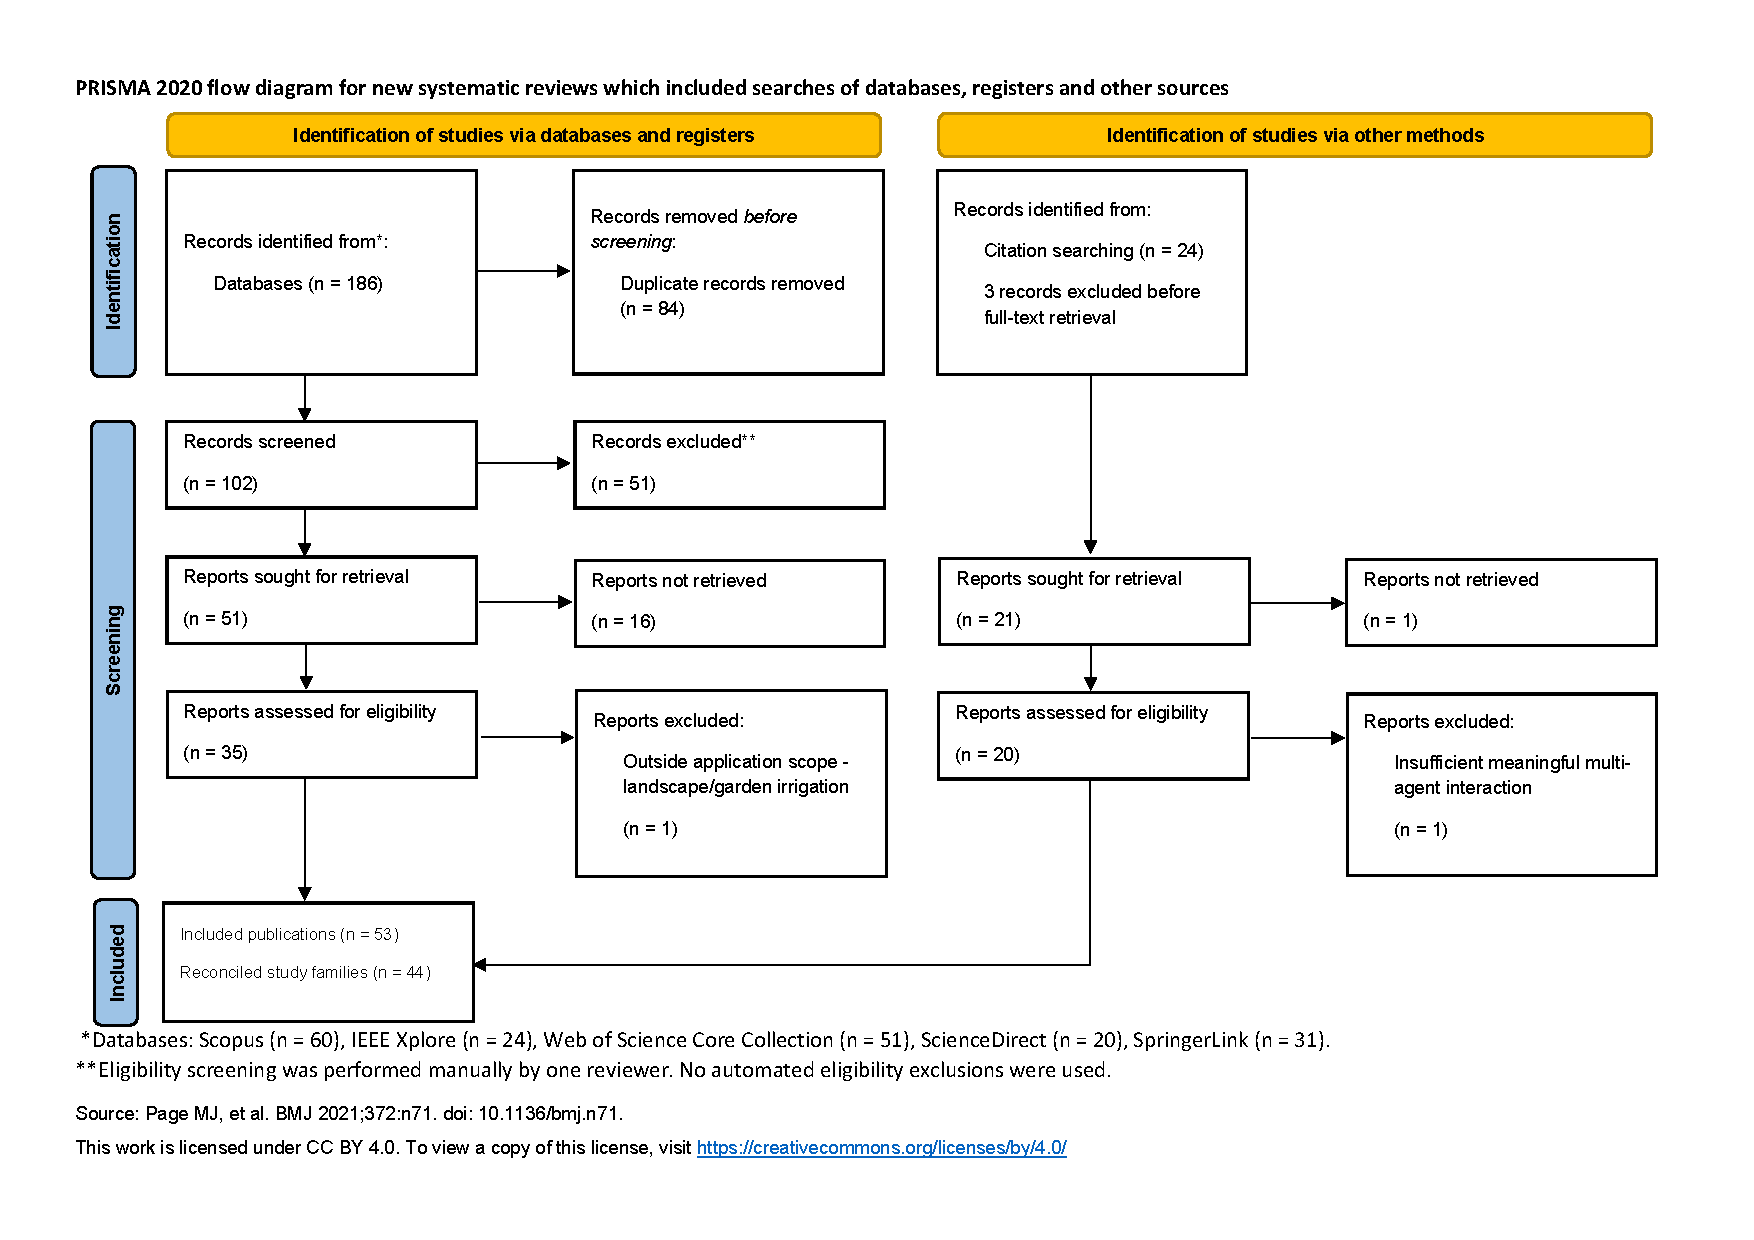
\includegraphics[
        width=\linewidth,
        height=0.88\textheight,
        keepaspectratio
    ]{PRISMA_2020_flow_diagram_FINAL}
    \caption{PRISMA 2020 study selection via five databases and
    supplementary citation searching: 53 included publications,
    subsequently reconciled into 44 study families. Adapted from
    Page et al. (2021), CC BY 4.0.}
    \label{fig:prisma2020}
\end{figure}
\end{landscape}
\clearpage

\subsection{Extraction, Quality Assessment and Synthesis}

Each included study was assigned an identification code (\texttt{S01-S53}), and its evidence was recorded in a \textbf{63-field} extraction dataset. 

In this review, coding refers to assigning predefined categories or labels to extracted information from each publication. Depending on the extraction field, a publication could receive either a single category or multiple categories.

The code book includes details about agricultural context, agent roles and structures, decision and coordination processes, constraints, outcomes, evaluation, and limitations. The information provided in the source was not mixed with those generated by the reviewer. Evidence locators and original comparator descriptions and outcomes were kept; \texttt{NR}, \texttt{NA} and \texttt{UNC} were used for missing, inapplicable, or uncertain information.

The seven quality-assessment criteria covered objectives, agent roles and autonomy, communication and coordination, environment and data, evaluation, reproducibility, and limitations. These were scored 0--2 individually, and added up to a possible score of 0--14. The categories with scores of 11--14,
7--10 and 0--6 were considered high, moderate, and limited methodological clarity, respectively. This assessment was descriptive, not an exclusion criteria nor a risk-of-bias or certainty-of-evidence assessment. Amongst the 53 publications analyzed, the mean score was \textbf{12.94/14} and the median score was \textbf{13}; \textbf{50} of them had high clarity, \textbf{3} were moderate and none had limited clarity.

Overlapping publications were identified if a system, model, or empirical case was reused. This resulted in \textbf{44 study families}: 37 single publications and seven multiple publications
(\texttt{SF05}, \texttt{SF08}, \texttt{SF13}, \texttt{SF16},
\texttt{SF25}, \texttt{SF42}, and \texttt{SF49}). For publication
statistics, $n=53$ applies, for family sensitivity analysis $n=44$
applies. Family categories can overlap and should not be confused with
replicated experiments.

The synthesis included the distribution of RQ1 agent roles and RQ2 coordination mechanisms, outcome-direction coding for RQ3, and assessment of evaluation and comparators for RQ4. Insights derived from the research questions contributed to the six axes of the MAS taxonomy. Selected ambiguities were verified with the original literature, but all 53 publications were not independently cross-checked. Variations in methodology, results and comparators prevented effect size synthesis. The References section of the report includes papers cited in the report. All data for the full set of 53 publications, including bibliography, extraction and quality assurance, screening, family mapping, and analysis are provided in the \href{https://github.com/ChayanTalukder/Multi-Agent-Systems-for-Sustainable-Smart-Farming} {public GitHub repository}.

\subsection{Characteristics of the Included Corpus}

The \textbf{53 articles} span 2001--2026. Five are pre-2010 landmark papers, 20 appeared between 2010 and 2019, and 28 between 2020 and 2026. \textbf{37} are journals, and \textbf{16} are conference proceedings articles. The median publication year is 2020, compared to 2022 for the original 34-paper database corpus, due to content inclusion through citation searching.

Table~\ref{tab:application_domains} shows the mutually exclusive primary application domains. Irrigation and water management accounts for the largest group (24/53). Family \texttt{SF42} spans two primary application domains, producing 45 family-category memberships across 44 families.

\begin{table}[H]
\centering
\small
\caption{Primary agricultural domains in the original and final corpora.}
\label{tab:application_domains}
\begin{tabularx}{\textwidth}{@{}Xrrr@{}}
\toprule
\textbf{Primary application domain} &
\textbf{Original 34} &
\textbf{Final 53} &
\textbf{Families} \\
\midrule
Irrigation / water management & 14 & 24 & 20 \\
Crop / farm management & 4 & 8 & 8 \\
Livestock / integrated farming & 5 & 6 & 6 \\
Workforce / robotics / task allocation & 5 & 6 & 4 \\
Energy / water--energy--food nexus & 4 & 5 & 3 \\
Soil / nutrient / environmental management & 2 & 4 & 4 \\
\midrule
\textbf{Total publications} & \textbf{34} & \textbf{53} & -- \\
\bottomrule
\end{tabularx}
\par\smallskip
\footnotesize\emph{Note:} Family memberships total 45 across 44
families because \texttt{SF42} spans two primary domains.
\end{table}

The scope of the integrated system was coded for \textbf{27/53} papers, resource constraints or limitations for \textbf{50/53}, and direct focus on sustainability for \textbf{39/53}. Coding refers to the topics that were covered, although it does not imply that positive results were achieved. 

In this review, simulation refers to the evaluation of a MAS within a modeled agricultural environment or scenario. A publication is described as simulation-coded when simulation is its assigned implementation-maturity category.


Simulation accounts for \textbf{46/53} implementation maturity categories (Table~\ref{tab:implementation_maturity}). There is a separate field on deployment status with 51 \emph{No}, 1 \emph{Yes}, and 1 \emph{Partial} entries; the reported \emph{Yes} case was not independently confirmed as sustained farm operation. Farm data and simulations alone do not establish implementation.

According to source reports, code was available in \textbf{8 out of 53}
cases and data in \textbf{14 out of 53} cases, but reproducibility was
not fully evaluated. Implications of the above evaluation settings are
discussed in RQ4.

\begin{table}[htbp]
\centering
\small
\caption{Implementation maturity coded for the 53 publications.}
\label{tab:implementation_maturity}
\begin{tabular}{lrr}
\toprule
\textbf{Maturity} & \textbf{Publications} & \textbf{Share} \\
\midrule
Simulation & 46 & 86.8\% \\
Prototype & 4 & 7.5\% \\
Field pilot & 2 & 3.8\% \\
Controlled experiment & 1 & 1.9\% \\
\midrule
\textbf{Total} & \textbf{53} & \textbf{100\%} \\
\bottomrule
\end{tabular}
\end{table}



% ==================================================
% 3. RESULTS: RQ0--RQ4 (CONDENSED, FROZEN 53/44 CORPUS)
% ==================================================
\section{Results: RQ0--RQ4}


\subsection{RQ0: MAS Application Landscape and Purpose}

\subsubsection{Applications and Functional Purposes}

RQ0 focuses on operational coordination and socio-ecological modeling
of farmers, resource users, and institutions. A single dominant functional purpose was assigned to each paper (Table~\ref{tab:rq0_functional_purposes}).
Allocation, scheduling, and control was the most common (21/53, 39.6\%);
policy and scenario assessment was next (17/53, 32.1\%), followed by
trading and resource management (13/53, 24.5\%). Decision support,
monitoring, or diagnosis came last (2/53, 3.8\%). The ranking is quite
similar among the 44 reconciled study families, despite the fact that the
families are not independent experiments.

\begin{table}[H]
\centering
\small
\caption{Dominant functional purpose of MAS in the initial
and final corpora, with study-family sensitivity counts.}
\label{tab:rq0_functional_purposes}

\begin{tabularx}{\textwidth}{@{}Xccc@{}}
\toprule

\textbf{Primary functional purpose} &
\textbf{Original 34} &
\textbf{Final 53} &
\textbf{44 families} \\

\midrule

Operational allocation, scheduling and control &
16 (47.1\%) & 21 (39.6\%) & 17 (38.6\%) \\

Policy, scenario and socio-ecological assessment &
9 (26.5\%) & 17 (32.1\%) & 15 (34.1\%) \\

Trading, negotiation and collective-resource governance &
7 (20.6\%) & 13 (24.5\%) & 10 (22.7\%) \\

Decision support, monitoring and diagnosis &
2 (5.9\%) & 2 (3.8\%) & 2 (4.5\%) \\

\midrule

\textbf{Total} & \textbf{34} & \textbf{53} & \textbf{44} \\

\bottomrule
\end{tabularx}

\par\smallskip
\begin{minipage}{\textwidth}
\footnotesize
\emph{Note:} Purpose categories are mutually exclusive
at the publication level. The family column reports
the reconciled evidence-presence classification and
must not be interpreted as independent replications.
\end{minipage}

\end{table}

The categories of irrigation and water management cover 24/53 documents
(20/44 families; Table~\ref{tab:application_domains}). They cover
areas like scheduling and distribution of water supply at the field level,
groundwater, and watershed management \parencite{chiewchan_water_2023,
jimenez_intelligent_2022,feuillette_sinuse_2003}. Other research documents focus on crop management, livestock and agriculture, energy management of dairy farms and greenhouses, soil and nutrient management, and harvest/worker coordination \parencite{catarino_fostering_2021,shah_peer--peer_2024,
harman_multi-agent_2022,grovermann_smart_2017}.


\subsubsection{Contributions and RQ0 Synthesis}

Contribution codes are multi-label: simulation/modeling and decision support, assessment or policy analysis each occur in 37/53 publications; optimisation/control in 27/53 articles; coordination/allocation/negotiation mechanism in 24/53 articles; and platforms/architectures in 22/53 articles. The integrated system is reported in 27/53 articles (25/44 families), but linking of the model components does not imply farm implementation.

In fact, the five pre-2010 foundational extensions stress on socio-ecological
assessments and collective resource governance. Operational
allocation is the dominant goal for articles written during 2020–2026 (15/28). These distinctions are specific to the retrieved corpus rather than reflecting a transition in the historical traditions of research. Hence, RQ0 indicates that MAS is applied to coordinate decision-making when resources are limited as well as to explore collective/policy scenarios.



% SECTION 3.2 — RQ1
% Revised prose; original Tables 4–6 retained.

\subsection{RQ1: Agent Types, Roles, Architectures and Decision-Making}

\subsubsection{Agent Roles and Architecture}

Agent roles were classified through manual classification of the study descriptions. The classifications are non-exclusive because a system may include multiple agents and/or multiple roles simultaneously (Table~\ref{tab:rq1_agent_roles}). Farmers, households or agricultural producers are found in 33 out of 53 studies, while managers, regulators or supervisors in 25/53 studies. Biophysics, crops, herds
or environmental components are represented in 19/53 studies, while operational field, irrigation, workforce or robot roles in 17/53 studies. Specialist advisory and market/trading roles are found in 11/53 studies. These figures are indicative of the represented roles; representation of a crop, herd or environment and is not necessarily an agent \parencite{gaudou_maelia_2014,harman_multi-agent_2022,
t_shanteer_cownet-ai_2026}.

\begin{table}[H]
\centering
\small

\caption{Manually adjudicated agent-role themes in the final corpus.}
\label{tab:rq1_agent_roles}

\begin{tabularx}{\textwidth}{@{}Xcc@{}}
\toprule

\textbf{Agent-role theme} &
\textbf{Publications ($n=53$)} &
\textbf{Families ($n=44$)} \\

\midrule

Farmer / household / agricultural producer &
33 (62.3\%) & 28 (63.6\%) \\

Manager / regulator / supervisory actor &
25 (47.2\%) & 19 (43.2\%) \\

Biophysical / herd / crop / environmental representation &
19 (35.8\%) & 17 (38.6\%) \\

Operational field / irrigation / workforce / robot actor &
17 (32.1\%) & 13 (29.5\%) \\

Specialist software / analytical / advisory actor &
11 (20.8\%) & 11 (25.0\%) \\

Market / bidder / trading role &
11 (20.8\%) & 8 (18.2\%) \\

\bottomrule
\end{tabularx}

\par\smallskip

\begin{minipage}{\textwidth}
\footnotesize
\emph{Note:} Categories are non-exclusive,
reviewer-adjudicated themes based on extracted descriptions.
A family contributes once to a role when at least one of
its publications supports that role. Biophysical
representation does not necessarily imply autonomous agency.
\end{minipage}

\end{table}

Architecture was divided according to decision-making power, and not according to the number of actors involved or whether it was implemented (Table~\ref{tab:rq1_architectures}). Decentralised designs constitute the largest source-coded category (17/53), with hybrid (13), hierarchical (11), centralised (10) and distributed (2) designs. Every publication had one
architecture code. Publications related to \texttt{SF42} were, on the
other hand, categorized as hybrid and hierarchical, resulting in 45 architecture codes within 44 families. The \emph{distributed} category is distinguished from the \emph{decentralised} category as seen in the extraction. These distributions reflect the corpus; they do not show that one architecture works better than another in all agricultural contexts \parencite{agyeman_semi-centralized_2025,therond_integrated_2014}.

\begin{table}[htbp]
\centering
\small

\caption{Frozen MAS architecture codes at publication
and study-family levels.}

\label{tab:rq1_architectures}

\begin{tabular}{lcc}
\toprule

\textbf{Architecture} &
\textbf{Publications ($n=53$)} &
\textbf{Families ($n=44$)} \\

\midrule

Decentralised & 17 (32.1\%) & 16 (36.4\%) \\

Hybrid & 13 (24.5\%) & 11 (25.0\%) \\

Hierarchical & 11 (20.8\%) & 9 (20.5\%) \\

Centralised & 10 (18.9\%) & 7 (15.9\%) \\

Distributed & 2 (3.8\%) & 2 (4.5\%) \\

\midrule

\textbf{Total publication codes} &
\textbf{53} & \textbf{--} \\

\bottomrule
\end{tabular}

\par\smallskip

\begin{minipage}{\textwidth}
\footnotesize
\emph{Note:} Architecture is exclusive for each
publication, but family evidence is not always exclusive.
\texttt{SF42} contains both hybrid and hierarchical
architecture coding in related publications; therefore
the family column sums to 45 category memberships across
44 families. The \emph{distributed} category is retained
separately from \emph{decentralised} as coded in
the extraction.
\end{minipage}

\end{table}

\subsubsection{Decision Paradigms and Autonomy}

The paradigms for decision-making of the agents are equally diverse
(Table~\ref{tab:rq1_paradigms}). Rule-based approaches are the most common (37/53), followed by economic or utility-based approaches
(20/53) and finally learning-based approaches (11/53). BDI and reactive
paradigms are used twice each; case-based and LLM-based approaches
once. Six publications do not provide information about a specific
approach. The approaches can be mixed, e.g., a rule-based approach
with economic goals and optimisation. An economic model of a
farming choice and learning-based approach to irrigation can
solve different problems \parencite{berger_agent-based_2001,grovermann_smart_2017,
agyeman_learning-based_2024}. The only paper that uses the LLM-based
advisory approach cannot be considered as proof for extensive
use of LLM agents in MAS \parencite{t_shanteer_cownet-ai_2026}.

\begin{table}[H]
\centering
\small

\caption{Source-coded decision paradigms in the
final corpus.}

\label{tab:rq1_paradigms}

\begin{tabularx}{\textwidth}{@{}Xcc@{}}
\toprule

\textbf{Decision paradigm} &
\textbf{Publications ($n=53$)} &
\textbf{Families ($n=44$)} \\

\midrule

Rule-based &
37 (69.8\%) & 31 (70.5\%) \\

Utility-based / economic &
20 (37.7\%) & 17 (38.6\%) \\

Learning-based &
11 (20.8\%) & 10 (22.7\%) \\

Belief--Desire--Intention (BDI) &
2 (3.8\%) & 1 (2.3\%) \\

Reactive &
2 (3.8\%) & 2 (4.5\%) \\

Case-based reasoning &
1 (1.9\%) & 1 (2.3\%) \\

Large language model (LLM)-based &
1 (1.9\%) & 1 (2.3\%) \\

Other &
1 (1.9\%) & 1 (2.3\%) \\

Not reported (NR) &
6 (11.3\%) & 5 (11.4\%) \\

\bottomrule
\end{tabularx}

\par\smallskip

\begin{minipage}{\textwidth}
\footnotesize
\emph{Note:} Decision paradigms are multi-label;
their percentages do not sum to 100\%.
\emph{Not reported} indicates a missing or unspecified
paradigm, not an additional decision-making approach.
Family counts record evidence found in any member publication.
\end{minipage}

\end{table}

No common valid scale of agent autonomy is applied to the articles.
Local decisions could still be dependent on a supervisor and a resource
constraint; central policy training could be followed up with local
implementation; optimizers can coordinate several agents without any direct
communication. In total, the findings related to
RQ1 suggest a variety of actors, decision processes and reasoning involved,
often within the resource or institutional constraints. But no agent
architecture has been proven to be superior to others and the reviewed corpus does not demonstrate a transition to fully autonomous farm operation.



% SECTION 3.3 — RQ2
% Prose revised; seven theme counts and table label unchanged.

\subsection{RQ2: Coordination, Cooperation, Negotiation and Resource Allocation}

\subsubsection{Communication and Adjudicated Mechanisms}

Several labels have been used in these studies to refer to processes and interactions between agricultural agents. Co-ordination is coded in 47/53 articles, information sharing in 33/53, communication in 30/53, competition in 23/53 and cooperation in 18/53. These overlapping codes only show what was reported; they do not identify any communication protocol or evidence that agents negotiated. We therefore reviewed the extracted descriptions of mechanisms and coded them into seven non-exclusive, manually adjudicated themes
(Table~\ref{tab:rq2_coordination_mechanisms}).  

Supervision or shared controller appears as the most common one (25/53),
interaction via a shared environment/resource follows (20/53). Operational
allocation, optimisation or scheduling occurs in 16/53 publications, 
auctions and other market interactions in 15/53, peer information sharing
in 13/53, learning or adaptation coordination/MARL in 9/53, and direct
negotiation/collective agreement in 8/53.

\begin{table}[H]
\centering
\small

\caption{Seven manually adjudicated coordination-mechanism
themes in the final MAS corpus.}

\label{tab:rq2_coordination_mechanisms}

\begin{tabularx}{\textwidth}{@{}Xcc@{}}
\toprule

\textbf{Coordination mechanism} &
\textbf{Publications ($n=53$)} &
\textbf{Families ($n=44$)} \\

\midrule

Hierarchical / supervisory / shared-controller &
25 (47.2\%) & 19 (43.2\%) \\

Environment- / shared-resource-mediated interaction &
20 (37.7\%) & 18 (40.9\%) \\

Operational allocation / optimisation / task scheduling &
16 (30.2\%) & 12 (27.3\%) \\

Auction / bidding / market / price-based exchange &
15 (28.3\%) & 10 (22.7\%) \\

Social-network diffusion / peer information exchange &
13 (24.5\%) & 13 (29.5\%) \\

Learning-based adaptive coordination / MARL &
9 (17.0\%) & 8 (18.2\%) \\

Direct negotiation / collective agreements &
8 (15.1\%) & 7 (15.9\%) \\

\bottomrule
\end{tabularx}

\par\smallskip

\begin{minipage}{\textwidth}
\footnotesize

\emph{Note:} Themes are non-exclusive. Family counts
indicate that at least one publication in the family
supports a theme and are not independent replications.
The direct-negotiation theme has a narrower, manually
reviewed definition than the original source-coded negotiation label (9 publications);
the two coding layers should not be numerically equated.

\end{minipage}

\end{table}

\subsubsection{Mechanism Boundaries and RQ2 Synthesis}

The distinction between whether interactions involve messages or a
common state is important for classifying coordination.
Agents can either communicate explicitly with each other, or influence
each other indirectly through their impact on the availability of
water, environmental conditions or a common state in general
\parencite{feuillette_sinuse_2003,becu_agent_2003,
barreteau_suitability_2004}. Special attention needs to be paid to
markets: an auction is able to allocate water or energy at a dairy farm
through bidding rules and does not require bilateral negotiation
\parencite{chiewchan_improving_2020,shah_peer--peer_2024}.
In the original extraction, negotiation was found in 9/53 articles,
while with manual adjudication 8/53 were categorized as negotiation or
collective agreements. These are different classification categories,
not substitutable measures. Similarly, centrally trained policies or task allocation by an optimiser do not, by themselves, establish direct agent-to-agent communication or decentralised decision authority at runtime.

Scarcity of resources or operational limitations were observed in 50/53
articles, although the ways in which these were solved differed.
Step 6H: cross-classification results revealed that all six articles on workforce/robots had some form of operational optimization and scheduling. Irrigation articles make use of different combinations, such as coordination, shared resources interaction, scheduling and agreements. The complete cross-classification matrices can be found in the \href{https://github.com/ChayanTalukder/Multi-Agent-Systems-for-Sustainable-Smart-Farming} {repository}. With regard to the study family level, the two evidence-presence counts are 19/44 for supervision and 18/44 for interaction.

Thus, the answers to RQ2 involve coordination through explicit and implicit
interaction, either used together within one multi-agent system or not.
These findings does not suggest a generally preferred method of coordination,
nor does coordination provide better results for farming.



% SECTION 3.4 — RQ3
% Prose revised; the original outcome-direction table and label are retained.

\subsection{RQ3: Agricultural, Resource-Efficiency, Livestock and Environmental Outcomes}

\subsubsection{Reported Outcomes and Evidence Direction}

Numerous articles report on agricultural or resource-based effects,
but reporting an effect does not prove that there was an improvement.
Agricultural outcomes were reported in 51/53 publications and resource
efficiency effects in 48/53. Environmental effects were reported in
38/53 articles and livestock-specific effects in 7/53. Environmental
mitigation mechanisms were reported in 41/53 articles, quantitative results
in 47/53 and trade-offs in 45/53. This is an overlapping set of indicators
for reporting effects rather than the number of effects.

In determining what the results actually indicate, the
outcome was considered using four mutually exclusive publication classes (Table~\ref{tab:rq3_outcome_direction}). Favourable results, typically conditional or simulation-based, comprise 24 of 53 publications. 21 out of 53 publications present mixed results depending on scenario or trade-offs;
seven are descriptive or feasibility-focused, while one does not consider a direct agricultural outcome. Related publications within the same study family may belong to different outcome-direction classes, thus the evidence presence counts for families are not disjoint.

\begin{table}[htbp]
\centering
\small

\caption{Adjudicated direction of reported RQ3 evidence.
Categories describe extracted conclusions, not pooled
causal effects.}

\label{tab:rq3_outcome_direction}

\begin{tabularx}{\textwidth}{@{}Xcc@{}}
\toprule

\textbf{Outcome-direction class} &
\textbf{Publications ($n=53$)} &
\textbf{Families ($n=44$)} \\

\midrule

Favourable, but conditional or simulated &
24 (45.3\%) & 19 (43.2\%) \\

Mixed, trade-off or scenario-dependent &
21 (39.6\%) & 21 (47.7\%) \\

Descriptive or feasibility; no directional conclusion &
7 (13.2\%) & 6 (13.6\%) \\

No directly evaluated agricultural outcome &
1 (1.9\%) & 1 (2.3\%) \\

\midrule

\textbf{Total publications} &
\textbf{53} & \textbf{--} \\

\bottomrule
\end{tabularx}

\par\smallskip

\begin{minipage}{\textwidth}
\footnotesize

\emph{Note:} Publication classes are mutually exclusive.
Family counts indicate evidence from any member publication;
a family may contain different outcome-direction classes.
The family entries therefore total 47 class memberships,
not 47 independent families. Favourable does not mean
field-validated or universally beneficial.

\end{minipage}

\end{table}

\subsubsection{Agricultural, Livestock and Resource Evidence}

The results obtained in the corpus differ greatly based on
applications. They include crop and yield cases, farm income, adoption
of technology, water requirement and availability, allocation equity,
electricity trading, and work performance. For example, some of the
findings explain the importance of the comparator and the scenario. In a
simulation of organic seeds and breeding policy, it was found that the gross
margin was lower for farms in certain scenarios \parencite{winter_assessing_2023}. In a study for harvest coordination, the source-checked comparator finished the tasks faster, while staffing considerations also played an important role in interpretation \parencite{harman_challenges_2023}. A study involving model predictive control for irrigation models compared simulated outcomes with heuristics \parencite{cobbenhagen_optimal_2022,schoonen_optimal_2019}.
Since both studies belong to \texttt{SF49}, they are one related evidence
line rather than two independent studies. Likewise, studies on water-scarcity  show that conclusions about efficiency and equity depend on the allocation objective and the scenarios considered \parencite{hung_assessing_2021,mahmoudian_adaptive_2025}.



Livestock uses should take special attention when defining
the measures that have been used. Electricity trading in dairy farms,
manure or resource exchange, and performance of advisory systems can be
studied without measuring animal health, or biological improvement
\parencite{shah_peer--peer_2024,shah_peer--peer_2026,
catarino_fostering_2021,t_shanteer_cownet-ai_2026}. Other works study
cases of water quality, soil, nutrients and pesticide management
\parencite{ng_agent-based_2011,quang_ex-ante_2014,
van_der_straeten_multi-agent_2010,grovermann_smart_2017}. Even if
precision irrigation, nutrient management or energy exchange have been
suggested as a means of mitigation, simulation results are not enough
to conclude about any emission reduction or pollution control.

\subsubsection{Trade-offs and RQ3 Synthesis}

A few identified implications concern conflicting priorities: water savings
could impact yields or access; environmental policies could lower
farm profits; staffing could vary with time required for the tasks;
efficient distribution could benefit different parties differently.
These conflicts can be identified either qualitatively or scenario-specifically
without necessarily being assessed as a Pareto surface. The
direction of an implication should therefore be understood along with
the assumptions, data, and comparisons made in the report.

Overall, the evidence on RQ3 indicates that MAS can be used to
analyze agricultural sustainability trade-offs, at times yielding
positive results against some alternative. No clear causal improvement of productivity, animal welfare, efficiency or environmental performance can be shown in practice by the evidence. Most of the evidence is heterogeneous and simulation-based.



% SECTION 3.5 — RQ4
% Prose revised; existing headings, references and Table 9 retained.

\subsection{RQ4: Evaluation Methods, Validation, Implementation Maturity and Limitations}

\subsubsection{Evaluation and Comparator Strength}

Model-based assessment dominates in studies of agricultural MAS.
Simulation accounts for 46/53 publications (39/44 study families). The remaining seven comprise four prototypes, two field pilots and one controlled experiment(Table~\ref{tab:implementation_maturity}). Implementation maturity
and deployment refer to different stages: a model may use real-world
weather or agricultural data without being implemented on a farm.
Settings discussed include policy and catchment scenarios,
irrigation and resource allocation benchmarks, energy market, and
workforce assignment for harvest \parencite{cobbenhagen_optimal_2022,
quang_ex-ante_2014,harman_multi-agent_2022}.

Comparator descriptions were recorded for 49/53 publications
(41/44 families). The count above includes simulated scenarios,
algorithms, calibration targets, and ambiguous/missing comparators.
Table~\ref{tab:rq4_comparator_interpretation}
illustrates how different references can be interpreted depending
on the conclusions made in the paper. For instance, better results
than an irrigation heuristic in simulations prove comparative
performance in the described settings, but a model calibrated for
real-world observations indicates plausibility. Neither proves
effectiveness in dynamic agricultural environments
\parencite{schoonen_optimal_2019,harman_challenges_2023}.

\begin{table}[htbp]
\centering
\scriptsize

\caption{Comparator and validation types and the
interpretations they can support in RQ4.}

\label{tab:rq4_comparator_interpretation}

\begin{tabularx}{\textwidth}{@{}XXX@{}}
\toprule

\textbf{Reference type} &
\textbf{Supported interpretation} &
\textbf{Important limitation} \\

\midrule

Competing algorithm or control policy &
Relative performance in the reported experiment &
Does not establish general superiority across farms \\

Historical or practice comparator &
Change relative to a documented practice &
May be confounded; not automatically causal \\

Scenario or policy counterfactual &
Differences within the specified model &
Not verified intervention impact in practice \\

Observed-data calibration or validation &
Plausibility or fit of model predictions &
Not proof that the proposed management improves sustainability \\

No clear comparator / not reported &
Descriptive or feasibility assessment &
Does not support a comparative-effectiveness claim \\

\bottomrule
\end{tabularx}
\end{table}

\subsubsection{Deployment, Reproducibility and Limitations}

The individual \texttt{Real\_World\_Deployment} field is noted
as \emph{No} for 51/53 studies, \emph{Yes} for \texttt{S02}, and
\emph{Partial} for \texttt{S06}. The one noted \emph{Yes} study
was not verified to represent sustained operation of the farm
\parencite{skobelev_smart_2019}; \texttt{S06} involves both physical
and virtual irrigation elements
\parencite{jimenez_intelligent_2022}. These codes cannot be treated
as verified long-term deployments.

Code availability was noted in 8/53 studies (8/44 families), and availability of data in 14/53 (13/44 families). These numbers characterize the source-acknowledged disclosure, not the execution and verification of the artefacts by someone. Also, reproducibility depends on parameters, software dependencies,
data provenance and scenario settings.

Among those coded by reviewers limitations, the necessity of validation
is present in 52/53 publications (43/44 families), uncertainty in 35/53,
reproducibility/data and environmental models in 18/53 each,
computational needs in 17/53, and scalability in 11/53.
The latter codes overlap and are different from author-identified
research gaps: 52/53 does not mean that 52 authors specifically wanted field trials.

To summarise, RQ4 reveals that agricultural MAS are primarily
evaluated using simulation, comparison of scenarios, and testing/calibration of algorithms. Such evaluations allow conclusions to be drawn on the basis of the assumptions made, but not evidence for transferable benefits under actual farm settings. High methodological clarity ratings and study family reconciliation facilitate evaluation of the literature. Neither can substitute for an independent field evaluation.




% ==================================================
% SECTION 4 — FORMAL MAS TAXONOMY AND EVIDENCE MAPPING
% Prose revised; taxonomy and evidence tables retained.
% ==================================================

\section{Formal MAS Taxonomy and Evidence Mapping}
\label{sec:taxonomy}

\subsection{Taxonomy Development}

This taxonomy was developed to allow a comparison of the included agricultural MAS without assuming that their application, internal structure and evaluation are of the same dimension. It is based on the frozen extraction of all 53 publications, organized into 44 study families, and includes the manual agent role (RQ1) and the coordination mechanism (RQ2) classifications. Each publication has one code for application domain, functional purpose and architecture. Role, decision paradigm and coordination mechanism may have multiple codes per publication.

For family-level counts, the category is considered to be present if at least one publication from this family refers to it. The counts reflect the distribution of the evidence across the related publications, not individual replications. Implementation maturity, outcome direction, comparator type and research artefact availability are evaluated independently as overlays of evidence. The resulting six-axis taxonomy is a descriptive categorization of this collection; it has not been externally validated as a general MAS classification.

\subsection{Formal MAS Taxonomy}

Table~\ref{tab:mas_taxonomy_axes} sets out the six design axes and
their coding rules. The corresponding publication and family
frequencies are presented with RQ0--RQ2 in Section~3.

\begin{table}[H]
\centering
\scriptsize
\caption{Six analytical axes of the evidence-grounded agricultural MAS taxonomy.}
\label{tab:mas_taxonomy_axes}
\begin{tabularx}{\textwidth}{@{}p{0.21\textwidth}Xp{0.22\textwidth}@{}}
\toprule
\textbf{Axis} & \textbf{What it describes} & \textbf{Publication coding} \\
\midrule
Application domain & Agricultural setting: irrigation, crops, livestock,
workforce, energy or soil/environment & Single-label \\
Functional purpose & Allocation/control, scenario assessment,
trading/governance or decision support & Single-label \\
Agent roles & Producers, supervisors, biophysical representations,
operational actors, advisers and traders & Multi-label; adjudicated \\
MAS architecture & Decentralised, hybrid, hierarchical, centralised
or distributed decision authority & Single-label \\
Decision paradigm & Rules, economic preferences, learning and
other agent decision logics & Multi-label \\
Coordination mechanism & Supervision, shared resources, scheduling,
markets, peer exchange, learning or negotiation & Multi-label; adjudicated \\
\bottomrule
\end{tabularx}
\end{table}

Each axis highlights one feature of the system, which includes the system's agricultural context, goal, roles of the agents involved, distribution of the authority of decision-making, decision-making rationale and mechanism of coordinating decisions. This distinction prevents the attribution of any feature on the basis of the name given to the system's architectural feature alone. Decentralization of decisions is not necessarily based on the exchange of messages directly, and agents controlled by one entity can still have their own decisions. The source-coded \emph{distributed} architecture is different from the \emph{decentralized}.

\subsection{Cross-Classification of MAS Characteristics}

The cross-classifications indicate which design options co-occur, not which designs work better. Of the 24 irrigation/water designs, 11 are operational, 8 deal with trading/governance, and 5 investigate policies/scenarios. 6 out of the 8 crop/farm designs study policy/scenario models; all 6 workforce/robotics
designs are operational. The architectural classification also vary by field. Irrigation uses all 5 classes, with 8 designs being decentralized and 8 hierarchical. Workforce/robots are mainly centralized (5/6); energy/WEF designs are mostly hybrid (4/5). These are features of the collected papers, not proof that the frequent design option is the best one \parencite{harman_multi-agent_2022,shah_peer--peer_2024}.

Within agent types and coordination methods, producer roles are accompanied by environment-mediated interaction in 20 papers, manager/regulator roles with supervisory coordination in 19, and trader roles with market coordination in 11 papers. Hierarchical architecture is also accompanied by supervisory coordination in 11 papers; decentralized architecture is accompanied by environment-mediated interaction in 9 papers. The codes are multi-valued, and thus these combinations do not imply causality. Papers within the same family can differ from each other as well: \texttt{SF42} includes both hybrid and hierarchical architecture codes. The complete cross-tabulation and family coding are stored in the Step 6H evidence map.

\subsection{Evidence Coverage Matrix}

The taxonomy provides an overview of where agricultural MAS design has been investigated; the evidence overlay provides details of how the studies were reviewed and what their outcome was. Table~\ref{tab:mas_domain_outcome} brings together the application domains along with implementation maturity and the adjudicated RQ3 outcome directions.

Irrigation/water management has the widest architectural
coverage, but 23 of its 24 publications are simulation-coded. Ten
have a positive but conditional outcome direction, while eleven give
mixed results. Not one of the 6 published papers on "Livestock/Integrated Farming" received a positive outcome direction.

The table characterises the available evidence, not causal treatment
effects. In particular, a favourable direction under a modeled
scenario or comparator does not establish a benefit in sustained farm
operation.

\begin{table}[H]
\centering
\scriptsize
\caption{Evidence overlay by primary agricultural domain (publication counts, $n=53$).}
\label{tab:mas_domain_outcome}
\setlength{\tabcolsep}{3.4pt}
\begin{tabularx}{\textwidth}{@{}>{\raggedright\arraybackslash}Xrrrrrr@{}}
\toprule
\textbf{Domain} & \textbf{$n$} & \textbf{Sim.} & \textbf{Fav.} &
\textbf{Mixed} & \textbf{Desc.} & \textbf{None} \\
\midrule
Irrigation / water & 24 & 23 & 10 & 11 & 3 & 0 \\
Crop / farm & 8 & 7 & 3 & 4 & 1 & 0 \\
Livestock / integrated & 6 & 4 & 0 & 2 & 3 & 1 \\
Workforce / robotics & 6 & 3 & 5 & 1 & 0 & 0 \\
Energy / WEF & 5 & 5 & 4 & 1 & 0 & 0 \\
Soil / nutrient / environment & 4 & 4 & 2 & 2 & 0 & 0 \\
\midrule
\textbf{Total} & \textbf{53} & \textbf{46} & \textbf{24} &
\textbf{21} & \textbf{7} & \textbf{1} \\
\bottomrule
\end{tabularx}
\par\smallskip
\footnotesize\emph{Note:} Sim. = simulation maturity; Fav. = favourable
but conditional/simulated; Mixed = mixed or scenario-dependent;
Desc. = descriptive/feasibility; None = no directly evaluated
agricultural outcome. Outcome-direction classes are mutually exclusive
at publication level. Favourable does not mean field-validated.
\end{table}

\subsection{Evidence Map and Coverage Gaps}

The Step 6H map at the family level shows the number of families supporting each design combination as \emph{absent} (zero), \emph{sparse} (one or two), \emph{moderate} (three to five) or \emph{dense} (six or more). This categorization is an indication of coverage; it does not reflect the study quality, utility or effectiveness.

The irrigation/water management area has the most comprehensive coverage
of MAS designs but is dominated by simulations. All the studies in
energy/WEF and soil, nutrients and environment areas are also simulation-based.
The absence or sparseness of cells alone cannot be the reason for doing
further studies in the areas of negotiation, MARL, distributed architecture and LLM agents, as some of the mechanisms might not be needed for the particular agricultural problem. The common problem across all the domains is the lack of evidence on field implementation, relevancy and results from a sustainability point of view. These problems have guided the research gap synthesis in Section~5.



% ==================================================
% SECTION 5 — INTEGRATED SYNTHESIS AND CONSOLIDATED RESEARCH GAPS
% Prose revised; original headings, citations, counts, and Table 12 preserved.
% ==================================================

\section{Integrated Synthesis and Consolidated Research Gaps}
\label{sec:integrated_synthesis}

\subsection{Cross-Research-Question Integration}

Overall, RQ0-RQ2 captures the design and orchestration of MAS for agriculture, while RQ3-RQ4 demonstrate how little evidence there is for impacts beyond modeled contexts. Water allocation, market and socio-ecological modeling deal with distinct sets of decisions, and a comparative ranking of their processes would be inappropriate. Rather, it would be more pertinent to investigate if these capabilities translate into sustainable gains for farming activities, resource utilization, and the environment.

\subsection{Publication-Level vs Study-Family Evidence}

The 53 publications were combined into 44 study families to accommodate overlapping publications due to related research products; seven of these families include more than one publication. For instance, the publications related to irrigation predictive control model belong to \texttt{SF49} and have the same evaluation line and are not independent confirmations
\parencite{cobbenhagen_optimal_2022,schoonen_optimal_2019}.
Similarly, harvest-allocation studies, \texttt{SF25}, need comparison with the papers specific to them. In contrast, MAELIA applications were not clustered merely because they were based on the same platform since the underlying model or case had to coincide as well.

Categories per family can also overlap. For example, \texttt{SF42} includes codes of hybrid and hierarchical architecture types within related publications. The main descriptive features remain after the reconciliation, yet family presence is only a sensitivity check, not an effect pool or 44 independent replicates of experiments.

\subsection{Outcome Direction and Comparator-Strength Assessment}

The adjudicated RQ3 findings comprise of 24 favorable but conditional or simulated articles, 21 mixed or scenario-dependent, seven descriptive or feasibility oriented, and one without a directly evaluated agricultural outcome (Table~\ref{tab:rq3_outcome_direction}). Categories are mutually exclusive; however, category presence for the family may overlap within relevant publications.

Even though 49 out of 53 publications have populated comparator-description field, it may refer to a simulated alternative, calibrated target, or unclear comparisons. This does not constitute 49 rigorously controlled assessments. The claims made based on the comparisons used, will differ (Table~\ref{tab:rq4_comparator_interpretation}). For instance, water allocation rules might trade-off profitability against fairness \parencite{mahmoudian_adaptive_2025} and harvesting allocation involves staff and completion time trade-offs \parencite{harman_challenges_2023}. Testing livestock advisory system does not, without animal measures, prove better welfare \parencite{t_shanteer_cownet-ai_2026}. Such interpretations are based on frozen extractions and targeted sources examination.

\subsection{Consolidated Research Gaps}

The gap assessment includes manual coding of author-identified needs,
Step 6H's coverage and maturity maps, and limitations identified
via RQ0-RQ4. Substantive author-gap text existed in 49 out of 53 papers
(four \texttt{NR}). The most common categories were those of uncertainty and
transferability (29/53), field or longitudinal validation (28/53),
stakeholder and behavioral validity (25/53), and biophysical or
environmental realism (23/53). Other gap topics were adaptive or
institutionally realistic coordination (19/53), scalability and sensing
(14/53), multiple resource management (12/53), and comparative evaluation
(9/53).

This set of author-gap themes should not be confused with reviewer-coded
limitations. In particular, the need for real-world validation was
identified in 52/53 papers, while the corresponding author theme
was identified in 28/53 papers. Code, data availability (8/53, 14/53)
along with variability in comparators contributed to the reproduction of
evaluation gaps. Empty taxonomy cells were not automatically coded as gaps.
Frequencies and supporting evidence can be found in Step 6I files in the \href{https://github.com/ChayanTalukder/Multi-Agent-Systems-for-Sustainable-Smart-Farming} {repository}.

\subsection{Prioritisation of Research Gaps}

Table~\ref{tab:integrated_gap_priorities} shows how the integrated hierarchy classifies six general quality-of-evidence issues as Priority A, and three context-dependent extensions as Priority B. Such classification does not depend on frequency or importance scoring, but rather takes into account convergence across author-reported needs, corpus coverage and evidence-strength appraisal.

\begin{table}[H]
\centering
\scriptsize
\caption{Frozen consolidated research-gap hierarchy (Step 6I).}
\label{tab:integrated_gap_priorities}
\setlength{\tabcolsep}{3pt}
\begin{tabularx}{\textwidth}{@{}p{0.08\textwidth}p{0.11\textwidth}X@{}}
\toprule
\textbf{Gap ID} & \textbf{Priority} & \textbf{Research gap} \\
\midrule
RG1 & A & Field, operational and longitudinal validation \\
RG2 & A & Robustness, uncertainty and transferability \\
RG3 & A & Behavioural, stakeholder and social validity \\
RG4 & A & Biophysical/environmental realism and long-horizon sustainability \\
RG5 & A & Reproducibility and transparent research artefacts \\
RG6 & A & Comparative evaluation and baseline quality \\
\midrule
RG7 & B & Scalability, sensing, computation and real-time operation \\
RG8 & B & Cross-domain and multi-resource integration \\
RG9 & B & Adaptive, distributed and institutionally realistic coordination \\
\bottomrule
\end{tabularx}
\end{table}

Priority A emphasises field and longitudinal validation, robustness,
credible stakeholder and environmental assumptions, reproducible
artefacts where permissible, and defensible comparators. Priority B
concerns operational scalability, integration of farm resources, and
adaptive or distributed coordination where the decision problem
justifies them. Additional agents, learning or negotiation should be
tested against simpler alternatives, not assumed to be improvements.




% ==================================================
% SECTION 6 — DISCUSSION
% Prose revised; original headings, citations and table reference retained.
% ==================================================

\section{Discussion}
\label{sec:discussion}

\subsection{Interpretation of Principal Findings}

From the existing literature two major applications of MAS in agriculture have been identified. The operational type of model, the type of analyses for coordination of irrigation, labour and other inputs, whereas socio-ecological models analyse decision-making of farmers and institutions under varying conditions of the environment and policies \parencite{chiewchan_improving_2020,berger_agent-based_2001,therond_integrated_2014}. As these applications have different objectives and outcome variables, to assess them using one performance criterion would be misleading. The citation search led to finding works on collective resource governance but was unable to identify any historical trend towards these applications.

\subsection{Architectural and Coordination Trade-offs}

The architectural choices influence which decisions are taken and how shared constraints are handled. A supervisory controller may be used for the common allocation; local agents may serve as representatives of the different owners, their preferences and information. Hybrid systems make use of the elements of both approaches, and impose integration needs. This is determined by the farm activity, sensing, communication reliability, institutional power and distribution effects. Coordination techniques also require accurate definitions: auctions may allocate resources according to the specified rules without bargaining, while water users may affect each other via the common resource without any communications \parencite{feuillette_sinuse_2003,becu_agent_2003,shah_peer--peer_2024}. No particular architecture or coordination technique is better than the others in all cases.

\subsection{Sustainability Evidence and Practical Implications}

For the interpretation of a sustainable outcome, it is necessary to understand whether something is different in relation to a certain comparative point based on specific assumptions. A good performance indicator does not necessarily mean increased productivity, equitable resource distribution, or better ecological condition. Articles discussing the predictive control of the related irrigation model \texttt{SF49} contrast simulation results with the
performance of heuristic-based plans \parencite{cobbenhagen_optimal_2022,
schoonen_optimal_2019}. However, they do not represent independent
evidence that such solutions work in the real farm environment. In the
same way, results about farm energy transactions, crop-livestock
interchanges, and advisory system performance do not show lower emissions or enhanced animal welfare \parencite{catarino_fostering_2021,t_shanteer_cownet-ai_2026}.

\subsection{Implications for Agricultural MAS Research}

The priorities listed in Table~\ref{tab:integrated_gap_priorities} are based on
the gap between model performance and demonstrated agricultural benefits. Evaluation should consider appropriate baselines, resource limitations, uncertain analyses, and consideration of gains and losses from resource allocation. Systems to be used on farms should have evaluations using working experience, preferably from multiple locations or seasons, documented through
proper data sources, software code, modeling parameters and scenarios where possible. Real-time sensing, multi-resource integration and adaptive or distributed resource allocation should be considered if they are necessary for farm decision making, not simply because they increase system complexity. The following sections consider validity threats and future research opportunities.





% ==================================================
% SECTION 7 — LIMITATIONS AND THREATS TO VALIDITY
% Prose revised; original subsection headings and evidence retained.
% ==================================================

\section{Limitations and Threats to Validity}

\subsection{Review-Process Limitations}

This systematic review process involved screening, extraction, and synthesis that was carried out by a single reviewer using a documented protocol and piloting criteria, as well as Rayyan software and manual coding to increase transparency. However, there was no independent verification, such as duplicate screening, checking for inter-reviewer agreement, or reviewing of all 53 articles in their full-text versions. Targeted searches may be affected by possible errors and by the reviewer's judgment.

Search was restricted to five chosen databases, search terms, and field limitations. The inclusion criteria allowed for peer-reviewed journals and conference publications in English, published between 2010--2026, and five papers prior to 2010 through the documented exception procedure. Backward/forward citation search included one generation. Additionally, \textbf{17 studies} were unavailable (16 through databases and one through citation search).

Protocols were maintained in a version-controlled way, although not registered elsewhere. An interpretation dated 12 October 2026 excludes irrigation of ornamental or public landscapes as it was not related to agriculture. The exact date of the Scopus V0.3c final run could not be traced back from the saved information.

\subsection{Limitations of the Included Evidence}

The majority of the studies were model-based: \textbf{46 out of 53
publications} showed simulation implementation maturity. Deployment
was reported separately as 51 \emph{No}, 1 \emph{Yes}
(\texttt{S02}, without independent verification of sustained
operations on farms) and 1 \emph{Partial} (\texttt{S06},
comprising both physical and virtual environment). Observational
data, calibration and prototypes must not be confused with validation
of normal operations.

Outcomes and comparators varied significantly. While the comparator
column was filled by \textbf{49 out of 53} publications, including simulated counterfactuals, heuristic benchmarks, calibration targets, and missing comparisons, but not 49 controlled trials. Positive results under these conditions cannot prove causal transferable benefits in production, efficiency, livestock welfare or sustainability.

The code and data availability was reported by \textbf{8 out of 53}
and \textbf{14 out of 53} publications, respectively. The seven-criteria QA score is a measure of methodological clarity rather than risk of bias of the
intervention. Thus, high methodological clarity scores cannot substitute rigorous comparators or field evidence.

\subsection{Evidence Dependence and Generalisability}

The \textbf{53 publications} were reduced to \textbf{44 study families}
since there exist some related systems or evaluations. The presence
checks at the family level keep the overall trends, but are not 44
independent experimental studies. This involved some assessment, and
related publications may have different categories assigned; the
\texttt{SF42} family includes hybrid and hierarchical architectures.

The coverage is highly variable in terms of farming environments,
with irrigation and water management in \textbf{24 out of 53} publications, whereas climate, hydrology, farm size, institution, and stakeholder behavior are different for each environment. Thus, this review is better suited for the claims about MAS evaluation and design rather than for general sustainability
benefits.



% ==================================================
% SECTION 8 — FUTURE RESEARCH DIRECTIONS
% Original headings, priorities and citations retained.
% ==================================================

\section{Future Research Directions}

These nine gaps identified in Table~\ref{tab:integrated_gap_priorities} will be the future research directions for agricultural MAS studies. Six Priority A gaps relate to issues of quality and generalisability, while three Priority B gaps relate to application-specific skills. The identified research directions are not benefits proven by the reviewed studies.

\subsection{Integrated Farm-Level Decision-Making}

In \textbf{RG8 (Priority B)}, research on integrated MAS is needed when there
are interactions between farm resources. For example, irrigation can have an impact on electricity use, crop water requirements, and labour requirements. Jointly coordinated approaches should be compared to simpler separate controls. The applications of integrated MAS for crop--livestock interaction and dairy-energy studies do not establish the superiority of the latter approach \parencite{catarino_fostering_2021,shah_peer--peer_2024}.

\textbf{RG3 (Priority A)} requires realistic farmer preferences, inequality of access, institutions, differences among stakeholders, and human involvement. These can be based on surveys, observed choices, or participatory research in places where this is possible; additional behavioural detail does not necessarily improve validity without empirical support. When property rights, local information, or institutional authority play a role in coordination, \textbf{RG9 (Priority B)} encourages comparing supervision, local rules, auctions, coordination, optimization, and learning approaches to implement simpler baselines.

\textbf{RG7 (Priority B)} asks for experimental evaluation of sensing inaccuracies, communication failures, delays, computational costs, and scalability. Such constraints may render a design unfeasible on a real farm.

\subsection{Robust Evaluation and Real-World Validation}

\textbf{RG1 (Priority A)} calls for prospective trials on farms,
preferably across different locations or seasons if possible. The
evaluations should indicate which parts of the MAS were involved, for
how long, and what agricultural variables were evaluated. Simulated inputs from farms should not be considered deployments.

\textbf{RG6 (Priority A)} requires an appropriate comparator based on
the claim: existing controllers or farm practices for operation
decisions, other algorithms for computational efficiency and explicit
assumptions of models for scenario counterfactuals
(Table~\ref{tab:rq4_comparator_interpretation}).
\textbf{RG2 (Priority A)} calls for sensitivity and transferability
tests in relation to weather, soil, crop type, market, resource
limitations, sensor uncertainty, behavior of stakeholders, including
failures and distributional considerations.

\textbf{RG5 (Priority A)} calls for documentation of software
version, codes if available, data sources, parameters, seeds,
baselines, and scenarios. Licensing or privacy constraints should be
stated even if the artifacts cannot be shared. Availability does not
guarantee independent reproducibility by itself.

\subsection{Resource and Environmental Sustainability Integration}

\textbf{RG4 (Priority A)} entails connections between agent choices,
hydrology, agronomy, soils, nutrients, livestock, resources and other
processes together with outcomes over an adequate time period. Less water
extraction should, for instance, be evaluated with respect to yield,
access to water and availability downstream. Energy-trading performance cannot stand in for measured emissions reductions, just as livestock advisory performance cannot establish improved animal welfare. Water allocation
and agricultural policy case studies explain why outcomes and comparators are needed \parencite{mahmoudian_adaptive_2025,grovermann_smart_2017}.

Long-horizon research should look at feedbacks, rebounds and conflicts
between conservation, productivity, income generation and fairness. This makes
\textbf{RG4} relevant to robustness (\textbf{RG2}), behavioural validity
(\textbf{RG3}) and the justification of multi-resource integration
(\textbf{RG8, Priority B}). Every model does not need all the subsystems of every farm.



% ==================================================
% SECTION 9 — CONCLUSION
% Prose revised; original heading and scientific findings retained.
% ==================================================

\section{Conclusion}

The current review analyzed 53 studies discovered via searches
of five databases and supplementary citation searching, with relevant
studies consolidated into 44 study groups. The agricultural MAS
were used for resource-limited decisions and socio-ecological/policy
scenarios. Irrigation and water management comprised the most
frequent domain of the system application (24/53). The differences
among the systems were in the agent roles, distribution of
the decision-making authority, rules, and economic modeling/learning.
The systems employed multiple types of coordination, including
supervision, interactions of shared resources, scheduling, markets,
exchange among peers, adaptive techniques and negotiation. The evidence did not establish any design as universally superior across agricultural settings.

However, caution is necessary regarding the findings about
the agricultural outcomes. Out of 53 studies, 24 showed favorable but
conditional or simulated agricultural outcomes, 21 – mixed or scenario-
specific, 7 – mostly descriptive or feasible studies, and 1 study
did not address an agricultural outcome. Given that 46/53 studies
are at maturity of simulation, there is still little independent evidence
about sustainable advantages in working farms.

The MAS taxonomic classification system based on its six axes, and the ranked RG1-RG9 research gaps helped to integrate these results. This is a foundation for future research into field validation, robustness, realism of the stakeholder and environmental systems, reproducibility, and enhanced comparison, without unnecessary system complexity.


% ==================================================
% DECLARATIONS AND SUPPLEMENTARY MATERIALS
% ==================================================

\section{Declarations and Supplementary Materials}

\par\medskip
\noindent\textbf{Funding and competing interests.}
This systematic literature review received no external
financial or non-financial support. The author declares
no competing interests.

\par\medskip
\noindent\textbf{Supplementary materials.}
The complete search strategies, extraction and quality-assessment
documentation, study-family reconciliation, PRISMA reporting
materials and supporting analyses are available in the
\href{https://github.com/ChayanTalukder/Multi-Agent-Systems-for-Sustainable-Smart-Farming} {public GitHub repository}.


\par\medskip
\noindent\textbf{Use of generative AI.}
OpenAI ChatGPT was used to support the organisation of project files, review workflows, consistency checks, academic revision, and LaTeX preparation. The assisted outputs were reviewed against the retained research records, with final responsibility for the methods, findings and conclusions remaining with the author.



% ==================================================
% REFERENCES
% ==================================================

\clearpage

% Print only publications explicitly cited in the report
\printbibliography[heading=bibintoc,title={References}]

% ==================================================
% APPENDICES (DISABLED FOR SHORT REPORT)
% ==================================================

% The complete appendices remain saved in appendices.tex.
% They are excluded from the shortened report.

% \clearpage
% \appendix
% % ==================================================
% APPENDICES A--D: upload this file and exact_search_queries.tex
% Requires: \usepackage{booktabs,tabularx,longtable,array,listings}
% Place % ==================================================
% APPENDICES A--D: upload this file and exact_search_queries.tex
% Requires: \usepackage{booktabs,tabularx,longtable,array,listings}
% Place % ==================================================
% APPENDICES A--D: upload this file and exact_search_queries.tex
% Requires: \usepackage{booktabs,tabularx,longtable,array,listings}
% Place \input{appendices} directly AFTER \appendix (exactly once)
% ==================================================
\section{Database Search Strategies}
\label{app:search}
The primary search followed frozen conceptual strategy V0.3c: an explicit MAS component, an agricultural setting, a focal farm/resource/environmental application and a coordination, allocation or decision function. A narrow recall branch addressed agricultural-MAS papers whose focal mechanism was more prominent in the abstract. Individual database syntax and search fields were translated and documented rather than assumed to be identical. The primary year window was 2010--2026.
\begin{table}[htbp]\centering\small
\caption{Final primary information sources and records exported before cross-database deduplication.}\label{tab:app_search_summary}
\begin{tabularx}{\textwidth}{@{}Xllr@{}}\toprule
Source & Final search date & Applied window/restriction & Records\\\midrule
Scopus & 29 Sep 2026 & English; article/conference; 2010--26 & 60\\
IEEE Xplore & 29 Sep 2026 & Journals/conferences; 2010--26 & 24\\
WoS Core Collection & 29--30 Sep 2026 & English; article/proceedings; 2010--26 & 51\\
ScienceDirect & 1 Oct 2026 & Year 2010--26; six-branch search & 20\\
SpringerLink & 1 Oct 2026 & English; article/conference; 2010--26 & 31\\
\midrule\textbf{Total}&&&\textbf{186}\\\bottomrule\end{tabularx}\end{table}
IEEE Xplore required two frozen branches (19 and six exports, with one overlap). ScienceDirect required six branches, producing 27 year-filtered branch retrievals and 20 unique records. SpringerLink required six branches; 44 year/language-filtered branch retrievals reduced to 33 unique records and then to 31 eligible article/conference records after excluding two chapter-only records. ScienceDirect did not apply a separate English-language search filter. The database-specific source logs document these adaptations and precision checks.
ACM Digital Library had initially been planned but was removed because the accessible search interface could not reproduce the frozen advanced title/abstract strategy. Relevant ACM publications remained eligible through other databases and supplementary citation searching. The 34 primary-pathway inclusions were used as seeds for one-generation backward and forward citation searching. Search records were retained privately where redistribution of database exports could be restricted.
\input{exact_search_queries.tex}
\clearpage
\section{Data Extraction and Quality Assessment Documentation}
\label{app:extraction}
The frozen publication-level extraction template contains 63 fields, with one row per included publication (\texttt{S01}--\texttt{S53}). The same version 1.0 codebook and seven-criterion methodological quality assessment (QA) were applied to the 34 database-pathway inclusions and 19 citation-search additions. The six source groupings A--F and general notes G in the schema are reproduced below as an audit-friendly field inventory. Full field definitions and category vocabularies remain in the project repository files \path{data_extraction/data_extraction_schema.md} and \path{data_extraction/extraction_codebook.md}. The final authoritative extraction dataset in the uploaded archive is \path{data_extraction/extraction_template_updated6(final).csv}.
\subsection{Extraction codebook and missing-value rules}
\texttt{NR} means not reported; \texttt{NA} means not applicable; and \texttt{UNC} means information is present but ambiguous. Multiple applicable values were separated by semicolons. Reviewer-coded classifications were distinguished from author-reported descriptions, and numerical results retained their original units and comparator contexts. Evidence locators record relevant pages, sections, tables or figures. A field populated with an outcome description does not itself demonstrate a beneficial effect.
\begingroup\footnotesize
\begin{longtable}{@{}p{0.28\textwidth}p{0.63\textwidth}@{}}
\caption{Inventory of the 63 extraction fields, following the frozen schema.}\label{tab:app_63_fields}\\
\toprule Field & Field purpose / information recorded \\\midrule\endfirsthead
\toprule Field & Field purpose / information recorded \\\midrule\endhead
\multicolumn{2}{@{}l}{\textbf{Study Identification and Descriptive Metadata}}\\\addlinespace[2pt]
\texttt{Study\_\allowbreak{}ID} & Unique SLR identifier assigned to the publication, e.g. S01--S53.\\
\texttt{Rayyan\_\allowbreak{}ID} & Rayyan record identifier from the final included-study export.\\
\texttt{PDF\_\allowbreak{}Filename} & Filename of the full-text PDF used for extraction.\\
\texttt{Title} & Full publication title.\\
\texttt{Authors} & Authors as recorded in the bibliographic metadata.\\
\texttt{Year} & Publication year.\\
\texttt{Venue} & Journal, conference, book, or other publication venue.\\
\texttt{Publication\_\allowbreak{}Type} & Publication type, such as journal article, conference paper, or book chapter.\\
\texttt{DOI} & Normalised DOI where available; otherwise NR.\\
\texttt{Geographical\_\allowbreak{}Context} & Country, region, farming area, or geographical setting studied, where applicable.\\
\texttt{Agricultural\_\allowbreak{}Domain} & Main agricultural context of the study, such as irrigation/water management, crops, livestock/dairy, greenhouse management, farm energy, workforce/harvesting, manure/nutrient management, land use, social-ecological systems, value chains, or integrated farming.\\
\texttt{Study\_\allowbreak{}Objective} & Concise summary of the research problem or objective addressed by the publication.\\
\texttt{Study\_\allowbreak{}Family\_\allowbreak{}ID} & Identifier linking publications confirmed to belong to the same research/system/experimental family. Publications without confirmed related papers receive their own family identifier.\\
\texttt{Related\_\allowbreak{}Publication\_\allowbreak{}IDs} & Other included Study\_ID values confirmed to be related to the same system, experiment, dataset, or research programme; otherwise NA.\\
\multicolumn{2}{@{}l}{\textbf{RQ0 --- Overall MAS Application and Scope}}\\\addlinespace[2pt]
\texttt{MAS\_\allowbreak{}Application\_\allowbreak{}Purpose} & Concise description of what the MAS is intended to accomplish in the agricultural system.\\
\texttt{System\_\allowbreak{}Integration\_\allowbreak{}Scope} & Whether the system addresses a single agricultural function, multiple connected functions, or a broader integrated farm/social-ecological system.\\
\texttt{Contribution\_\allowbreak{}Type} & Main contribution of the publication, such as MAS architecture, algorithm, simulation model, decision-support framework, coordination mechanism, optimisation method, control system, or implemented platform.\\
\texttt{Implementation\_\allowbreak{}Maturity} & Stage at which the proposed MAS is demonstrated, such as conceptual/model-level, simulation, prototype, controlled experiment, field pilot, or operational deployment.\\
\multicolumn{2}{@{}l}{\textbf{RQ1 --- MAS Architectures, Agent Roles, and Decision-Making}}\\\addlinespace[2pt]
\texttt{Agent\_\allowbreak{}Types} & Types of agents represented in the system, such as farmer, crop, field, irrigation, water/resource, livestock, pasture, sensor, machinery, energy, market, coordinator, or environmental agents.\\
\texttt{Agent\_\allowbreak{}Roles} & Main responsibilities and functions assigned to the identified agents.\\
\texttt{MAS\_\allowbreak{}Architecture} & Overall organisational architecture of the MAS, such as centralised, decentralised, distributed, hierarchical, or hybrid.\\
\texttt{Agent\_\allowbreak{}Paradigm} & Agent design paradigm where identifiable, such as reactive, rule-based, utility-based, BDI, learning-based, or other explicitly described architecture.\\
\texttt{Decision\_\allowbreak{}Mechanism} & Main mechanism used by agents to make decisions, such as rules, optimisation, planning, machine learning, reinforcement learning, MARL, MPC, auction-based decision making, or hybrid methods.\\
\texttt{Agent\_\allowbreak{}Autonomy\_\allowbreak{}Description} & Description of what decisions agents can make independently and where central or external control remains.\\
\texttt{Input\_\allowbreak{}Information} & Information used by agents for decision-making, such as sensor measurements, weather, soil moisture, crop demand, prices, livestock state, resource availability, or forecasts.\\
\texttt{MAS\_\allowbreak{}Platform\_\allowbreak{}Technology} & Implementation or simulation technologies reported, such as JADE, GAMA, MATLAB, Python, custom MAS platforms, IoT infrastructure, or other frameworks.\\
\texttt{RQ1\_\allowbreak{}Evidence\_\allowbreak{}Locator} & Page, section, table, or figure locations supporting the main RQ1 extraction.\\
\multicolumn{2}{@{}l}{\textbf{RQ2 --- Communication, Coordination, Negotiation, and Resource Management}}\\\addlinespace[2pt]
\texttt{Interaction\_\allowbreak{}Type} & Forms of inter-agent interaction, such as communication, information sharing, cooperation, coordination, negotiation, competition, or task allocation.\\
\texttt{Coordination\_\allowbreak{}Mechanism} & Mechanism used to coordinate agents, such as priority rules, utility-based allocation, auctions, contract-net protocols, consensus, optimisation, scheduling, market mechanisms, MARL, or other approaches.\\
\texttt{Communication\_\allowbreak{}Mechanism} & How agents exchange information, such as direct messages, peer-to-peer exchange, agent communication protocols, shared environments, blackboards, markets, or indirect interaction.\\
\texttt{Information\_\allowbreak{}Shared} & Information exchanged among agents, such as resource requests, offers, bids, demand, availability, prices, sensor information, environmental state, or task status.\\
\texttt{Managed\_\allowbreak{}Resource\_\allowbreak{}or\_\allowbreak{}Task} & Resource or coordination target being managed, such as water, irrigation capacity, energy, feed, pasture, land, manure, machinery, labour/workforce, harvest tasks, or other farm resources/tasks.\\
\texttt{Resource\_\allowbreak{}Scarcity\_\allowbreak{}or\_\allowbreak{}Constraint\_\allowbreak{}Modelled} & Whether limited availability, capacity, scarcity, competition, scheduling constraints, or comparable resource/task constraints are explicitly represented.\\
\texttt{Allocation\_\allowbreak{}or\_\allowbreak{}Coordination\_\allowbreak{}Objective} & Objective guiding coordination or allocation, such as efficiency, productivity, cost, profit, fairness, welfare, sustainability, resource utilisation, conflict reduction, or multi-objective optimisation.\\
\texttt{Conflict\_\allowbreak{}Resolution} & Method used to resolve incompatible requests, competing objectives, resource conflicts, or task conflicts; NR or NA where appropriate.\\
\texttt{Competing\_\allowbreak{}Agents\_\allowbreak{}or\_\allowbreak{}Demands} & Agents, stakeholders, farms, crops, livestock groups, tasks, or other demands competing for limited resources or attention.\\
\texttt{Irrigation\_\allowbreak{}Decision\_\allowbreak{}Inputs} & For irrigation/water studies, information used in irrigation or water-allocation decisions, including soil moisture, crop water requirements, crop stress, rainfall, forecasts, drought, reservoir availability, or irrigation capacity. Use NA for non-irrigation studies.\\
\texttt{RQ2\_\allowbreak{}Evidence\_\allowbreak{}Locator} & Page, section, table, or figure locations supporting the main RQ2 extraction.\\
\multicolumn{2}{@{}l}{\textbf{RQ3 --- Agricultural, Livestock, Resource-Efficiency, and Environmental Outcomes}}\\\addlinespace[2pt]
\texttt{Agricultural\_\allowbreak{}Outcomes} & Reported agricultural outcomes such as crop yield, crop health, crop stress, irrigation performance, production, unmet demand, farm utility, or productivity.\\
\texttt{Livestock\_\allowbreak{}Outcomes} & Reported livestock-related outcomes such as water demand, feed demand, animal health, heat stress, grazing, pasture allocation, welfare, or dairy-farm performance. Use NA when livestock is outside the study scope.\\
\texttt{Resource\_\allowbreak{}Efficiency\_\allowbreak{}Outcomes} & Reported effects on water use, irrigation efficiency, energy use, resource utilisation, allocation fairness, workload, scheduling efficiency, or resource conflicts.\\
\texttt{Environmental\_\allowbreak{}Outcomes} & Reported environmental effects such as freshwater consumption, water scarcity, greenhouse-gas emissions, CO2, CH4, N2O, manure impacts, energy consumption, fertiliser use, nutrient runoff, pollution, soil condition, land use, pasture, carbon resources, or ecosystem effects.\\
\texttt{Environmental\_\allowbreak{}Mitigation\_\allowbreak{}Mechanism} & Mechanisms intended to reduce environmental impact, such as precision irrigation, demand-aware allocation, manure management, renewable-energy scheduling, improved feeding, nutrient management, grazing management, or carbon-aware decisions.\\
\texttt{Sustainability\_\allowbreak{}Addressed} & Degree to which sustainability is substantively addressed: direct, indirect, or not addressed. Detailed coding rules will be defined in the codebook.\\
\texttt{Quantitative\_\allowbreak{}Results} & Key numerical results relevant to RQ3, recorded with the values, units, and comparison context reported by the authors.\\
\texttt{Tradeoffs\_\allowbreak{}Reported} & Explicitly reported trade-offs between productivity, welfare, cost, resource efficiency, fairness, environmental performance, or other objectives.\\
\texttt{RQ3\_\allowbreak{}Evidence\_\allowbreak{}Locator} & Page, section, table, or figure locations supporting the main RQ3 extraction.\\
\multicolumn{2}{@{}l}{\textbf{RQ4 --- Evaluation, Limitations, and Research Gaps}}\\\addlinespace[2pt]
\texttt{Evaluation\_\allowbreak{}Type} & Main evaluation method, such as simulation, analytical evaluation, case study, controlled experiment, laboratory experiment, field experiment, pilot deployment, or real-world deployment.\\
\texttt{Evaluation\_\allowbreak{}Environment} & Description of the farm, simulation, IoT, laboratory, field, social-ecological, or other environment used for evaluation.\\
\texttt{Data\_\allowbreak{}Source} & Origin of evaluation data, such as synthetic data, simulation-generated data, real sensor data, farm data, public datasets, historical data, surveys, or mixed sources.\\
\texttt{Experimental\_\allowbreak{}Scenarios} & Scenarios or conditions evaluated, such as normal operation, drought, scarcity, changing demand, uncertain environments, heat stress, different resource levels, or alternative management strategies.\\
\texttt{Baselines\_\allowbreak{}Comparators} & Algorithms, policies, existing practices, non-MAS approaches, control strategies, or other baselines used for comparison.\\
\texttt{Evaluation\_\allowbreak{}Metrics} & Metrics used to assess system or algorithm performance, such as accuracy, reward, latency, task success, computational performance, or other reported evaluation measures.\\
\texttt{Evaluation\_\allowbreak{}Results} & Qualitative or quantitative MAS/system evaluation results, including algorithmic performance, baseline comparisons, or ablation results distinct from agricultural and environmental outcomes.\\
\texttt{Evaluation\_\allowbreak{}Scale} & Scale of evaluation where reported, such as number of agents, farms, fields, animals, tasks, resources, simulation duration, geographical extent, or number of scenarios.\\
\texttt{Real\_\allowbreak{}World\_\allowbreak{}Deployment} & Whether the system was evaluated in an actual operational or field setting rather than solely through simulation or synthetic experiments.\\
\texttt{Code\_\allowbreak{}Available} & Whether implementation/source code is publicly available or explicitly provided.\\
\texttt{Data\_\allowbreak{}Available} & Whether the dataset or sufficient underlying evaluation data are publicly available or explicitly provided.\\
\texttt{Limitation\_\allowbreak{}Categories} & Standardised categories assigned to limitations discussed or clearly evidenced in the publication, including scalability, uncertainty, explainability, interoperability, environmental modelling, computational requirements, reproducibility/data availability, deployment cost, real-world validation/adoption, or other limitations.\\
\texttt{Reported\_\allowbreak{}Limitations} & Limitations, constraints, or threats to validity explicitly reported by the authors.\\
\texttt{Reported\_\allowbreak{}Research\_\allowbreak{}Gaps} & Future work, unresolved problems, open challenges, or research gaps explicitly identified by the publication.\\
\texttt{RQ4\_\allowbreak{}Evidence\_\allowbreak{}Locator} & Page, section, table, or figure locations supporting the main RQ4 extraction.\\
\multicolumn{2}{@{}l}{\textbf{General Extraction Notes}}\\\addlinespace[2pt]
\texttt{Extraction\_\allowbreak{}Notes} & Short reviewer notes for unusual cases, ambiguous classifications, relationships between publications, or extraction decisions that require later verification.\\
\bottomrule\end{longtable}\endgroup
\subsection{Quality assessment}
Each criterion was scored 0 (insufficient), 1 (partially addressed) or 2 (clearly addressed), for an overall score from 0 to 14. QA supported descriptive assessment of methodological clarity and did not automatically exclude studies or replace a formal intervention-specific risk-of-bias instrument.
\begin{table}[htbp]\centering\small
\caption{Seven frozen quality-assessment criteria.}\label{tab:app_qa_criteria}
\begin{tabularx}{\textwidth}{@{}llX@{}}\toprule Code & Criterion & Main assessment question \\\midrule
QA1 & Research objective & Is the problem or objective clearly defined?\\
QA2 & Agent roles/autonomy & Are agent responsibilities and autonomy described?\\
QA3 & Communication/coordination & Are interaction/coordination procedures specified?\\
QA4 & Environment/data & Are agricultural setting and inputs adequately described?\\
QA5 & Evaluation & Is the evaluation clear and meaningful for the study?\\
QA6 & Reproducibility & Are methods, parameters and implementation sufficiently detailed?\\
QA7 & Limitations & Are study limitations meaningfully discussed?\\
\bottomrule\end{tabularx}\end{table}
The final assessment covered all 53 publications: 50 in the high-clarity band (11--14), three in the moderate band (7--10) and none in the limited band (0--6). The mean QA total was 12.94/14 and the median 13/14. Criterion-level results, totals and written justification are retained in \path{data_extraction/quality_assessment_updated6(final).csv.csv}. These scores do not establish real-world effectiveness, experimental causal validity or independent reproducibility.

\section{Study-Family Reconciliation}
\label{app:families}
The 53 publication records were reconciled into 44 study families, consisting of 37 single-publication and seven multi-publication families. A shared platform, topic or author group was insufficient on its own to justify grouping: substantial reuse of an empirical case, model experiment or dataset, or an explicit publication extension, was required. The complete S-ID--SF-ID mapping is reproduced in Table~\ref{tab:app_family_mapping}. Its canonical source files in the uploaded repository are \path{data_extraction/study_family_reconciliation_53.csv} and \path{data_extraction/study_family_summary_44.csv}.
\begin{table}[htbp]\centering\small
\caption{Multi-publication study families (seven families; 16 related publications).}\label{tab:app_multifamilies}
\begin{tabularx}{\textwidth}{@{}llX@{}}\toprule Family & Publication IDs & Reconciliation basis \\\midrule
SF05 & S05, S11, S29 & Dairy P2P energy / MAPDES publication line\\
SF08 & S08, S23 & Semi-centralised MARL irrigation\\
SF13 & S13, S22 & Core MAELIA platform\\
SF16 & S16, S20 & Community irrigation negotiation\\
SF25 & S25, S33, S34 & Harvest workforce and task allocation\\
SF42 & S42, S52 & Aveyron MAELIA application and WEF extension\\
SF49 & S49, S53 & Multi-agent irrigation MPC/MARA conference and journal reports\\
\bottomrule\end{tabularx}\end{table}
\begingroup\footnotesize
\begin{longtable}{@{}p{0.08\textwidth}p{0.09\textwidth}p{0.08\textwidth}p{0.64\textwidth}@{}}
\caption{Complete publication identifier, study-family identifier and title mapping.}\label{tab:app_family_mapping}\\
\toprule S-ID & SF-ID & Year & Publication title \\\midrule\endfirsthead
\toprule S-ID & SF-ID & Year & Publication title \\\midrule\endhead
\texttt{S01} & \texttt{SF01} & 2018 & Polarization in (post)nomadic resource use in Eastern Morocco: insights using a multi-agent simulation model\\
\texttt{S02} & \texttt{SF02} & 2019 & Smart Farming -- Open Multi-agent Platform and Eco-System of Smart Services for Precision Farming\\
\texttt{S03} & \texttt{SF03} & 2023 & Assessing seed and breeding interventions for organic farming using a multiagent value chain approach\\
\texttt{S04} & \texttt{SF04} & 2026 & CowNet-AI: A Multi-Agent Decision Support Framework for Social Network--Driven Welfare Insights in Dairy Cattle\\
\texttt{S05} & \texttt{SF05} & 2024 & Peer-to-peer energy trading in dairy farms using multi-agent systems\\
\texttt{S06} & \texttt{SF06} & 2022 & Intelligent IoT-multiagent precision irrigation approach for improving water use efficiency in irrigation systems at farm and district scales\\
\texttt{S07} & \texttt{SF07} & 2024 & Learning-based multi-agent MPC for irrigation scheduling\\
\texttt{S08} & \texttt{SF08} & 2025 & A semi-centralized multi-agent RL framework for efficient irrigation scheduling\\
\texttt{S09} & \texttt{SF09} & 2024 & Energy management for demand response in networked greenhouses with multi-agent deep reinforcement learning\\
\texttt{S10} & \texttt{SF10} & 2011 & CaTMAS: A multi-agent model for simulating the dynamics of carbon resources of West African villages\\
\texttt{S11} & \texttt{SF05} & 2026 & Peer-to-peer energy trading in dairy farms using multi-agent reinforcement learning\\
\texttt{S12} & \texttt{SF12} & 2023 & MASSAI: Multi-agent system for simulating sustainable agricultural intensification of smallholder farms in Africa\\
\texttt{S13} & \texttt{SF13} & 2014 & Integrated modelling of social-ecological systems: The MAELIA high-resolution multi-agent platform to deal with water scarcity problems\\
\texttt{S14} & \texttt{SF14} & 2019 & Network-aware multi-agent simulations of herder-farmer conflicts\\
\texttt{S15} & \texttt{SF15} & 2017 & Modelling a multi agent system for dairy farms for integrated decision making\\
\texttt{S16} & \texttt{SF16} & 2023 & Water distribution in community irrigation using a multi-agent system\\
\texttt{S17} & \texttt{SF17} & 2026 & Assessment of agricultural vulnerability and risk to climate change in sugarcane production through life cycle analysis and a multi-agent system\\
\texttt{S18} & \texttt{SF18} & 2026 & Quantum Machine Learning-Enhanced Multiagent Reinforcement Learning for Intelligent Crop Resource Allocation in IoT-Enabled Smart Agriculture\\
\texttt{S19} & \texttt{SF19} & 2024 & Modification of the Ant Colony Optimization Algorithm for Solving Multi-Agent Task Allocation Problem in Agricultural Application\\
\texttt{S20} & \texttt{SF16} & 2020 & Improving Water Allocation Using Multi-agent Negotiation Mechanisms\\
\texttt{S21} & \texttt{SF21} & 2026 & AI-driven multi-agent framework for smart irrigation and crop health monitoring in Indian rice and sugarcane farming\\
\texttt{S22} & \texttt{SF13} & 2014 & The MAELIA Multi-agent platform for integrated analysis of interactions between agricultural land-use and low-water management strategies\\
\texttt{S23} & \texttt{SF08} & 2024 & Semi-centralized Multi-agent RL for Irrigation Scheduling\\
\texttt{S24} & \texttt{SF24} & 2019 & Intelligent multi-agent system for water reduction in automotive irrigation processes\\
\texttt{S25} & \texttt{SF25} & 2023 & Challenges for Multi-Agent Based Agricultural Workforce Management\\
\texttt{S26} & \texttt{SF26} & 2021 & Assessing Adaptive Irrigation Impacts on Water Scarcity in Nonstationary Environments---A Multi-Agent Reinforcement Learning Approach\\
\texttt{S27} & \texttt{SF27} & 2013 & Multi-agent agro-economic simulation of irrigation water demand with climate services for climate change adaptation\\
\texttt{S28} & \texttt{SF28} & 2010 & A multi-agent simulation model for spatial optimisation of manure allocation\\
\texttt{S29} & \texttt{SF05} & 2024 & A Multi-agent Systems Approach for Peer-to-Peer Energy Trading in Dairy Farming\\
\texttt{S30} & \texttt{SF30} & 2018 & Heterogeneous multi-agent resource allocation through multi-bidding with applications to precision agriculture\\
\texttt{S31} & \texttt{SF31} & 2022 & Dynamic Task Allocation Method for Heterogenous Multiagent System in Uncertain Scenarios of Agricultural Field Operation\\
\texttt{S32} & \texttt{SF32} & 2012 & A constrained multi-agent system compensating for self-lucrative behaviours in water resource sharing\\
\texttt{S33} & \texttt{SF25} & 2022 & Multi-agent task allocation for harvest management\\
\texttt{S34} & \texttt{SF25} & 2022 & Multi-Agent Task Allocation Techniques for Harvest Team Formation\\
\texttt{S35} & \texttt{SF35} & 2011 & An agent-based simulation model of human--environment interactions in agricultural systems\\
\texttt{S36} & \texttt{SF36} & 2017 & 'Smart' policies to reduce pesticide use and avoid income trade-offs: An agent-based model applied to Thai agriculture\\
\texttt{S37} & \texttt{SF37} & 2014 & Ex-ante assessment of soil conservation methods in the uplands of Vietnam: An agent-based modeling approach\\
\texttt{S38} & \texttt{SF38} & 2017 & An agent-based simulation of cooperation in the use of irrigation systems\\
\texttt{S39} & \texttt{SF39} & 2020 & Water management for irrigation, crop yield and social attitudes: a socio-agricultural agent-based model to explore a collective action problem\\
\texttt{S40} & \texttt{SF40} & 2011 & An agent-based model of farmer decision-making and water quality impacts at the watershed scale under markets for carbon allowances and a second-generation biofuel crop\\
\texttt{S41} & \texttt{SF41} & 2018 & A hybrid TOPSIS-agent-based framework for reducing the water demand requested by stakeholders with considering the agents' characteristics and optimization of cropping pattern\\
\texttt{S42} & \texttt{SF42} & 2014 & Fine spatio-temporal simulation of cropping and farming systems effects on irrigation withdrawal dynamics within a river basin\\
\texttt{S43} & \texttt{SF43} & 2001 & Agent-based spatial models applied to agriculture: a simulation tool for technology diffusion, resource use changes and policy analysis\\
\texttt{S44} & \texttt{SF44} & 2003 & SINUSE: A multi-agent model to negotiate water demand management on a free access water table\\
\texttt{S45} & \texttt{SF45} & 2003 & Agent based simulation of a small catchment water management in northern Thailand: Description of the CATCHSCAPE model\\
\texttt{S46} & \texttt{SF46} & 2004 & Suitability of Multi-Agent Simulations to study irrigated system viability: application to case studies in the Senegal River Valley\\
\texttt{S47} & \texttt{SF47} & 2007 & Simulating soil fertility and poverty dynamics in Uganda: A bio-economic multi-agent systems approach\\
\texttt{S48} & \texttt{SF48} & 2025 & An adaptive multi-agent model for water allocation under scarcity: application of bankruptcy methods\\
\texttt{S49} & \texttt{SF49} & 2022 & Optimal Irrigation Allocation for Large-Scale Arable Farming\\
\texttt{S50} & \texttt{SF50} & 2023 & Multi-Robot Task Allocation in Agriculture Scenarios Based on the Improved NSGA-II Algorithm\\
\texttt{S51} & \texttt{SF51} & 2021 & Fostering local crop-livestock integration via legume exchanges using an innovative integrated assessment and modelling approach based on the MAELIA platform\\
\texttt{S52} & \texttt{SF42} & 2024 & Multi-actor approach to manage the water-energy-food nexus at territory scale\\
\texttt{S53} & \texttt{SF49} & 2019 & Optimal irrigation management for large-scale arable farming using model predictive control\\
\bottomrule\end{longtable}\endgroup
Within the MAELIA line, the core platform is \texttt{SF13}; the Aveyron/WEF application is \texttt{SF42}; and the independent Vend\'ee crop--livestock application remains \texttt{SF51}. MP-MAS applications with distinct case studies were not collapsed solely due to platform reuse. The related irrigation-MPC publications \texttt{S49} and \texttt{S53} form \texttt{SF49}; a platform overview does not count as an independent confirmation of another included application\'s numerical results. The unretrieved SHADOC reference is not a member of the included corpus.
Study-family counts use any-member evidence for multi-label categories, which can overlap. \texttt{SF42}, for example, contributes evidence to both hybrid and hierarchical architecture categories. Family presence is not a statistical meta-analysis or a demonstration of independent replication.
\clearpage
\section{PRISMA 2020 Checklist and Supplementary Reporting}
\label{app:prisma}
The flow diagram appears in Section~4, and the detailed PRISMA 2020 audit is summarised below. The latest supplied repository includes the source diagram at \path{analysis/PRISMA_2020_flow_diagram_FINAL.pdf} and the audit at \path{analysis/SLR_7_PRISMA_2020_reporting_audit_FINAL.xlsx}. This is a project-specific reporting-location and completion audit, not a substitute for the official checklist, which includes additional sub-items. The complete official checklist and abstract guidance are available at \url{https://www.prisma-statement.org/prisma-2020-checklist}. The PRISMA 2020 statement is Page et al. (2021; \url{https://doi.org/10.1136/bmj.n71}).
\subsection{Study-selection flow reconciliation}
\begin{table}[htbp]\centering\small
\caption{Final PRISMA stage counts (two search pathways).}\label{tab:app_prisma_counts}
\begin{tabularx}{\textwidth}{@{}Xrr@{}}\toprule Stage & Database pathway & Citation pathway \\\midrule
Records identified & 186 & 24\\
Duplicates removed prior to screening & 84 & --\\
Records screened / new candidates & 102 & 24\\
Records excluded before retrieval & 51 & 3\\
Reports sought for full text & 51 & 21\\
Reports not retrieved & 16 & 1\\
Reports assessed at full text & 35 & 20\\
Reports excluded at full text & 1 & 1\\
Reports included & 34 & 19\\
\midrule \textbf{Total included publications} & \multicolumn{2}{c}{\textbf{53}}\\
\textbf{Reconciled study families} & \multicolumn{2}{c}{\textbf{44}}\\
\bottomrule\end{tabularx}\end{table}
The database pathway comprised 60 Scopus, 24 IEEE Xplore, 51 Web of Science, 20 ScienceDirect and 31 SpringerLink records. Across both pathways, 72 full-text reports were sought, 17 were not retrieved, 55 were assessed and two were excluded after full-text assessment. The 44-family figure is an additional evidence-independence count, not asserted as identical to the PRISMA concept of studies.
\subsection{Full-text exclusions and protocol deviations}
\begin{table}[htbp]\centering\footnotesize
\caption{Traceable supplementary exclusions and retrieval exceptions.}\label{tab:app_exceptions}
\begin{tabularx}{\textwidth}{@{}p{0.2\textwidth}X@{}}\toprule Stage & Document / status and rationale \\\midrule
Primary full-text exclusion & Isern et al. (2012), \emph{Development of a multi-agent system simulation platform for irrigation scheduling with case studies for garden irrigation}; excluded for landscape/garden irrigation outside the agricultural-production scope.\\
Citation full-text exclusion & B08, \emph{A new BDI agent architecture based on the belief theory. Application to the modelling of cropping plan decision-making}; insufficient meaningful multi-agent interaction.\\
Citation report not retrieved & B13, \emph{SHADOC: a multi-agent model to tackle viability of irrigated systems}; full text unavailable, therefore not assessed and not a substantive exclusion.\\
Citation pre-retrieval exclusions & B10: insufficient connected multi-agent interaction; B11: book chapter outside publication-type scope; B18: non-peer-reviewed/internal document.\\
\bottomrule\end{tabularx}\end{table}
ACM Digital Library was omitted from primary searches due to restricted advanced search capability; the late garden-irrigation application clarification was logged on 12 October 2026. No automation-based eligibility exclusions or study registers were used. The review was conducted by one reviewer and was not externally registered. Versioned protocol and amendment notes were retained in the repository.
\subsection{PRISMA 2020 reporting-location checklist}
\begingroup\footnotesize
\begin{longtable}{@{}p{0.075\textwidth}p{0.35\textwidth}p{0.48\textwidth}@{}}
\caption{Project reporting audit against the 27 main PRISMA 2020 checklist items.}\label{tab:app_prisma_checklist}\\
\toprule Item & Topic & Location / completion note \\\midrule\endfirsthead
\toprule Item & Topic & Location / completion note \\\midrule\endhead
1 & Title & Title page; systematic literature review explicitly identified.\\
2 & Abstract & Completed abstract on title page.\\
3 & Rationale & Section 1.\\
4 & Objectives & Section 1.3, RQ0--RQ4.\\
5 & Eligibility criteria & Section 3.3 and protocol/inclusion\_exclusion.md.\\
6 & Information sources & Section 3.2; Appendix A search dates and sources.\\
7 & Search strategy & Appendix A exact field-specific Boolean strings and filters.\\
8 & Selection process & Sections 3.4--3.6; single-reviewer Rayyan workflow.\\
9 & Data collection process & Sections 3.7--3.8; Appendix B.\\
10 & Data items & Appendix B 63-field extraction inventory.\\
11 & Risk of bias assessment & Methodological QA used, not a formal RoB instrument; Sections 3.8, 9.\\
12 & Effect measures & No common/pooled effect measures; Sections 3.10 and 5.\\
13 & Synthesis methods & Sections 3.9--3.10 and 5--7.\\
14 & Reporting-bias assessment & No formal publication/reporting-bias test; declared in Appendix D.4.\\
15 & Certainty assessment & No GRADE-style certainty assessment; declared in Appendix D.4.\\
16 & Study selection & Section 4 and Appendix D; 53 included publications.\\
17 & Study characteristics & Sections 4--6 and Appendix C.\\
18 & Risk of bias in studies & Present QA as methodological quality, not formal RoB; Sections 4.5, 5.5.\\
19 & Individual study results & Section 5 with evidence-backed examples; study-level extraction retained.\\
20 & Results of syntheses & Sections 5--7.\\
21 & Reporting biases & No formal reporting-bias assessment performed.\\
22 & Certainty of evidence & No formal certainty framework applied.\\
23 & Discussion & Sections 8--10, including limitations and future directions.\\
24 & Registration and protocol & Not externally registered; version-controlled protocol and amendments.\\
25 & Support & Funding and support declaration in Appendix D.4.\\
26 & Competing interests & Competing-interests declaration in Appendix D.4.\\
27 & Availability of data/code & Public repository and material-availability declaration in Appendix D.4.\\
\bottomrule\end{longtable}\endgroup
\subsection{Required final declarations and material availability}
\noindent\textbf{Registration.} This review was not registered in an external systematic-review registry. The protocol and subsequent amendments were version-controlled in the project repository.
\par\noindent\textbf{Funding and support.}
This systematic literature review received no external
financial or non-financial support.
\par\noindent\textbf{Competing interests.}
The author declares no competing interests.
\par\noindent\textbf{Data, code and materials.}
The review protocol, database-search documentation,
extraction schema and codebook, final extraction and
quality-assessment datasets, study-family reconciliation,
evidence synthesis and PRISMA reporting materials are
available in the public project repository:

\href{https://github.com/ChayanTalukder/Multi-Agent-Systems-for-Sustainable-Smart-Farming/tree/main}{Public GitHub project repository}

Publisher PDFs and licensed database exports are not
redistributed publicly. The repository documents the
review and its analytical materials; it does not imply
that all included MAS implementations are reproducible
from publicly available software.
\par\noindent\textbf{Evidence-assessment limitations.} No formal intervention-specific risk-of-bias instrument, GRADE certainty assessment or statistical publication-bias test was performed. Reviewer-coded methodological QA, targeted source checks and conservative comparator/outcome adjudication were used instead.
 directly AFTER \appendix (exactly once)
% ==================================================
\section{Database Search Strategies}
\label{app:search}
The primary search followed frozen conceptual strategy V0.3c: an explicit MAS component, an agricultural setting, a focal farm/resource/environmental application and a coordination, allocation or decision function. A narrow recall branch addressed agricultural-MAS papers whose focal mechanism was more prominent in the abstract. Individual database syntax and search fields were translated and documented rather than assumed to be identical. The primary year window was 2010--2026.
\begin{table}[htbp]\centering\small
\caption{Final primary information sources and records exported before cross-database deduplication.}\label{tab:app_search_summary}
\begin{tabularx}{\textwidth}{@{}Xllr@{}}\toprule
Source & Final search date & Applied window/restriction & Records\\\midrule
Scopus & 29 Sep 2026 & English; article/conference; 2010--26 & 60\\
IEEE Xplore & 29 Sep 2026 & Journals/conferences; 2010--26 & 24\\
WoS Core Collection & 29--30 Sep 2026 & English; article/proceedings; 2010--26 & 51\\
ScienceDirect & 1 Oct 2026 & Year 2010--26; six-branch search & 20\\
SpringerLink & 1 Oct 2026 & English; article/conference; 2010--26 & 31\\
\midrule\textbf{Total}&&&\textbf{186}\\\bottomrule\end{tabularx}\end{table}
IEEE Xplore required two frozen branches (19 and six exports, with one overlap). ScienceDirect required six branches, producing 27 year-filtered branch retrievals and 20 unique records. SpringerLink required six branches; 44 year/language-filtered branch retrievals reduced to 33 unique records and then to 31 eligible article/conference records after excluding two chapter-only records. ScienceDirect did not apply a separate English-language search filter. The database-specific source logs document these adaptations and precision checks.
ACM Digital Library had initially been planned but was removed because the accessible search interface could not reproduce the frozen advanced title/abstract strategy. Relevant ACM publications remained eligible through other databases and supplementary citation searching. The 34 primary-pathway inclusions were used as seeds for one-generation backward and forward citation searching. Search records were retained privately where redistribution of database exports could be restricted.
\subsection{Exact database-specific search expressions}

The following Boolean strings are reproduced from the final frozen query logs, preserving the field-specific branch syntax. The search filters and count reconciliations are shown above. These expressions document the completed searches; they are not a proposal to rerun the review.

\subsubsection{Scopus: V0.3c (29 September 2026)}

\paragraph{Final frozen expression}

\begin{lstlisting}

(
    TITLE(
        "multi-agent system*" OR
        "multi agent system*" OR
        "multiagent system*" OR
        "multi-agent" OR
        multiagent*
    )

    AND

    TITLE-ABS(
        agricultur* OR
        farming OR
        "smart farm*" OR
        "smart farming" OR
        "precision agriculture" OR
        "precision farming" OR
        irrigat* OR
        livestock OR
        "precision livestock" OR
        dairy OR
        cattle OR
        crop* OR
        pasture OR
        grazing OR
        farmer* OR
        grain*
    )

    AND

    TITLE(
        irrigat* OR
        "irrigation water" OR
        "water allocation" OR
        "water distribution" OR
        "water sharing" OR
        "water management" OR
        "water demand" OR
        "water scarcity" OR
        "soil moisture" OR

        livestock OR
        "precision livestock" OR
        dairy OR
        cattle OR
        herd* OR
        pasture OR
        grazing OR
        manure OR
        "animal welfare" OR

        "resource allocation" OR
        "resource sharing" OR
        "resource negotiation" OR
        "resource scheduling" OR
        "task allocation" OR

        "environmental sustainability" OR
        "climate adaptation" OR
        "climate mitigation" OR
        emission* OR
        methane OR
        "greenhouse gas*" OR
        "renewable energy" OR
        "energy management" OR
        "energy trading" OR
        "nutrient management" OR
        runoff OR
        "soil health" OR
        "soil degradation" OR
        "agricultural waste" OR
        "farm waste" OR
        microclimate
    )

    AND

    TITLE-ABS(
        coordinat* OR
        cooperat* OR
        negotiat* OR
        allocat* OR
        schedul* OR
        "resource sharing" OR
        "resource management" OR
        "decision support" OR
        "decision-making" OR
        "decision making" OR
        "integrated decision*" OR
        "distributed decision*" OR
        "collective decision*" OR
        "distributed control" OR
        "adaptive control" OR
        "peer-to-peer" OR
        auction* OR
        consensus
    )
)

OR

(
    TITLE(
        agricultur* OR
        farming OR
        "smart farm*" OR
        "smart farming" OR
        "precision agriculture"
    )

    AND

    TITLE(
        "multi-agent system*" OR
        "multi agent system*" OR
        "multiagent system*" OR
        "multi-agent" OR
        multiagent*
    )

    AND

    ABS(
        irrigat* OR
        fertiliz* OR
        harvest* OR
        livestock OR
        dairy OR
        pasture OR
        manure OR
        "resource allocation" OR
        "resource sharing" OR
        "resource scheduling" OR
        "energy management" OR
        "energy trading" OR
        "renewable energy" OR
        "climate adaptation" OR
        "climate mitigation" OR
        emission*
    )

    AND

    ABS(
        coordinat* OR
        cooperat* OR
        negotiat* OR
        allocat* OR
        schedul* OR
        "decision support" OR
        "decision-making" OR
        "decision making" OR
        "distributed control" OR
        "adaptive control" OR
        "tracking control"
    )
)

\end{lstlisting}

\subsubsection{IEEE Xplore: V0.3c-A and V0.3c-B (29 September 2026)}

\paragraph{Branch A: main MAS pathway (repaired final version)}

\begin{lstlisting}

(
    (
        "Document Title":"multi-agent"
        OR "Document Title":multiagent
    )

    AND

    (
        "Document Title":agriculture
        OR "Abstract":agriculture
        OR "Document Title":agricultural
        OR "Abstract":agricultural
        OR "Document Title":farming
        OR "Abstract":farming
        OR "Document Title":"smart farming"
        OR "Abstract":"smart farming"
        OR "Document Title":"precision agriculture"
        OR "Abstract":"precision agriculture"
        OR "Document Title":irrigation
        OR "Abstract":irrigation
        OR "Document Title":livestock
        OR "Abstract":livestock
        OR "Document Title":dairy
        OR "Abstract":dairy
        OR "Document Title":cattle
        OR "Abstract":cattle
        OR "Document Title":crop
        OR "Abstract":crop
        OR "Document Title":pasture
        OR "Abstract":pasture
        OR "Document Title":grain
        OR "Abstract":grain
    )

    AND

    (
        "Document Title":irrigation
        OR "Document Title":"water allocation"
        OR "Document Title":"water distribution"
        OR "Document Title":"water management"
        OR "Document Title":"water scarcity"
        OR "Document Title":"soil moisture"
        OR "Document Title":livestock
        OR "Document Title":dairy
        OR "Document Title":cattle
        OR "Document Title":pasture
        OR "Document Title":grazing
        OR "Document Title":manure
        OR "Document Title":"resource allocation"
        OR "Document Title":"resource sharing"
        OR "Document Title":"resource negotiation"
        OR "Document Title":"resource scheduling"
        OR "Document Title":"task allocation"
        OR "Document Title":"environmental sustainability"
        OR "Document Title":"climate adaptation"
        OR "Document Title":emission
        OR "Document Title":methane
        OR "Document Title":"renewable energy"
        OR "Document Title":"energy management"
        OR "Document Title":"nutrient management"
        OR "Document Title":microclimate
    )

    AND

    (
        "All Metadata":coordination
        OR "All Metadata":cooperation
        OR "All Metadata":negotiation
        OR "All Metadata":allocation
        OR "All Metadata":scheduling
        OR "All Metadata":"resource sharing"
        OR "All Metadata":"resource management"
        OR "All Metadata":"decision support"
        OR "All Metadata":"decision making"
        OR "All Metadata":"distributed control"
        OR "All Metadata":"adaptive control"
        OR "All Metadata":"peer-to-peer"
        OR "All Metadata":auction
        OR "All Metadata":consensus
        OR "All Metadata":control
    )
)

\end{lstlisting}

\paragraph{Branch B: narrow recall branch}

\begin{lstlisting}

(
    (
        "Document Title":agriculture
        OR "Document Title":agricultural
        OR "Document Title":farming
        OR "Document Title":"smart farming"
        OR "Document Title":"precision agriculture"
    )

    AND

    (
        "Document Title":"multi-agent"
        OR "Document Title":multiagent
    )

    AND

    (
        "Abstract":irrigation
        OR "Abstract":fertilizer
        OR "Abstract":fertilization
        OR "Abstract":harvest
        OR "Abstract":livestock
        OR "Abstract":dairy
        OR "Abstract":pasture
        OR "Abstract":manure
        OR "Abstract":"resource allocation"
        OR "Abstract":"resource sharing"
        OR "Abstract":"resource scheduling"
        OR "Abstract":"energy management"
        OR "Abstract":"energy trading"
        OR "Abstract":"renewable energy"
        OR "Abstract":"climate adaptation"
        OR "Abstract":emission
    )

    AND

    (
        "Abstract":coordination
        OR "Abstract":cooperation
        OR "Abstract":negotiation
        OR "Abstract":allocation
        OR "Abstract":scheduling
        OR "Abstract":"decision support"
        OR "Abstract":"decision making"
        OR "Abstract":"distributed control"
        OR "Abstract":"adaptive control"
        OR "Abstract":"tracking control"
    )
)

\end{lstlisting}

\noindent The two branch exports contained 19 and six records respectively, with one overlap: $19+6-1=24$ unique IEEE records.

\subsubsection{Web of Science Core Collection: V0.3c (29--30 September 2026)}

\paragraph{Final frozen advanced-search expression}

\begin{lstlisting}

(
    TI=(
        "multi-agent system*" OR
        "multi agent system*" OR
        "multiagent system*" OR
        "multi-agent" OR
        multiagent*
    )

    AND

    (
        TI=(
            agricultur* OR
            farming OR
            "smart farm*" OR
            "smart farming" OR
            "precision agriculture" OR
            "precision farming" OR
            irrigat* OR
            livestock OR
            "precision livestock" OR
            dairy OR
            cattle OR
            crop* OR
            pasture OR
            grazing OR
            farmer* OR
            grain*
        )

        OR

        AB=(
            agricultur* OR
            farming OR
            "smart farm*" OR
            "smart farming" OR
            "precision agriculture" OR
            "precision farming" OR
            irrigat* OR
            livestock OR
            "precision livestock" OR
            dairy OR
            cattle OR
            crop* OR
            pasture OR
            grazing OR
            farmer* OR
            grain*
        )
    )

    AND

    TI=(
        irrigat* OR
        "irrigation water" OR
        "water allocation" OR
        "water distribution" OR
        "water sharing" OR
        "water management" OR
        "water demand" OR
        "water scarcity" OR
        "soil moisture" OR

        livestock OR
        "precision livestock" OR
        dairy OR
        cattle OR
        herd* OR
        pasture OR
        grazing OR
        manure OR
        "animal welfare" OR

        "resource allocation" OR
        "resource sharing" OR
        "resource negotiation" OR
        "resource scheduling" OR
        "task allocation" OR

        "environmental sustainability" OR
        "climate adaptation" OR
        "climate mitigation" OR
        emission* OR
        methane OR
        "greenhouse gas*" OR
        "renewable energy" OR
        "energy management" OR
        "energy trading" OR
        "nutrient management" OR
        runoff OR
        "soil health" OR
        "soil degradation" OR
        "agricultural waste" OR
        "farm waste" OR
        microclimate
    )

    AND

    (
        TI=(
            coordinat* OR
            cooperat* OR
            negotiat* OR
            allocat* OR
            schedul* OR
            "resource sharing" OR
            "resource management" OR
            "decision support" OR
            "decision-making" OR
            "decision making" OR
            "integrated decision*" OR
            "distributed decision*" OR
            "collective decision*" OR
            "distributed control" OR
            "adaptive control" OR
            "peer-to-peer" OR
            auction* OR
            consensus
        )

        OR

        AB=(
            coordinat* OR
            cooperat* OR
            negotiat* OR
            allocat* OR
            schedul* OR
            "resource sharing" OR
            "resource management" OR
            "decision support" OR
            "decision-making" OR
            "decision making" OR
            "integrated decision*" OR
            "distributed decision*" OR
            "collective decision*" OR
            "distributed control" OR
            "adaptive control" OR
            "peer-to-peer" OR
            auction* OR
            consensus
        )
    )
)

OR

(
    TI=(
        agricultur* OR
        farming OR
        "smart farm*" OR
        "smart farming" OR
        "precision agriculture"
    )

    AND

    TI=(
        "multi-agent system*" OR
        "multi agent system*" OR
        "multiagent system*" OR
        "multi-agent" OR
        multiagent*
    )

    AND

    AB=(
        irrigat* OR
        fertiliz* OR
        harvest* OR
        livestock OR
        dairy OR
        pasture OR
        manure OR
        "resource allocation" OR
        "resource sharing" OR
        "resource scheduling" OR
        "energy management" OR
        "energy trading" OR
        "renewable energy" OR
        "climate adaptation" OR
        "climate mitigation" OR
        emission*
    )

    AND

    AB=(
        coordinat* OR
        cooperat* OR
        negotiat* OR
        allocat* OR
        schedul* OR
        "decision support" OR
        "decision-making" OR
        "decision making" OR
        "distributed control" OR
        "adaptive control" OR
        "tracking control"
    )
)

\end{lstlisting}

\subsubsection{ScienceDirect (1 October 2026)}

The interface required six separately executed two-field branches. In each branch, the first expression was entered in the \emph{Title} field and the second in \emph{Title, abstract or author-specified keywords}. The final unique union was $A1 \cup A2r \cup A3 \cup A4 \cup B1 \cup B2$.

\paragraph{Branch A1}

\paragraph{Title field}

\begin{lstlisting}

(
    "multi-agent"
    OR multiagent
)
AND
(
    irrigation
    OR water
    OR livestock
    OR dairy
    OR "soil moisture"
)

\end{lstlisting}

\paragraph{Title, abstract or author-specified keywords}

\begin{lstlisting}

(
    agriculture
    OR farming
    OR crop
)
AND
(
    coordination
    OR allocation
    OR scheduling
    OR control
    OR decision
)

\end{lstlisting}

\paragraph{Branch A2r}

\paragraph{Title field}

\begin{lstlisting}

(
    "multi-agent"
    OR multiagent
)
AND
(
    resource
    OR energy
    OR climate
)

\end{lstlisting}

\paragraph{Title, abstract or author-specified keywords}

\begin{lstlisting}

(
    agriculture
    OR farming
    OR livestock
    OR dairy
)
AND
(
    coordination
    OR allocation
    OR control
    OR decision
    OR trading
)

\end{lstlisting}

\paragraph{Branch A3}

\paragraph{Title field}

\begin{lstlisting}

(
    "multi-agent"
    OR multiagent
)
AND
(
    emission
    OR methane
    OR nutrient
    OR runoff
    OR soil
    OR waste
)

\end{lstlisting}

\paragraph{Title, abstract or author-specified keywords}

\begin{lstlisting}

(
    agriculture
    OR farming
    OR crop
)
AND
(
    coordination
    OR allocation
    OR control
    OR decision
)

\end{lstlisting}

\paragraph{Branch A4}

\paragraph{Title field}

\begin{lstlisting}

(
    "multi-agent"
    OR multiagent
)
AND
(
    pasture
    OR grazing
    OR manure
    OR welfare
    OR microclimate
)

\end{lstlisting}

\paragraph{Title, abstract or author-specified keywords}

\begin{lstlisting}

(
    agriculture
    OR farming
    OR livestock
    OR dairy
)
AND
(
    coordination
    OR allocation
    OR control
    OR decision
    OR welfare
)

\end{lstlisting}

\paragraph{Branch B1}

\paragraph{Title field}

\begin{lstlisting}

(
    "multi-agent"
    OR multiagent
)
AND
(
    agriculture
    OR farming
)

\end{lstlisting}

\paragraph{Title, abstract or author-specified keywords}

\begin{lstlisting}

(
    irrigation
    OR fertilizer
    OR harvest
    OR livestock
    OR dairy
)
AND
(
    coordination
    OR control
    OR decision
)

\end{lstlisting}

\paragraph{Branch B2}

\paragraph{Title field}

\begin{lstlisting}

(
    "multi-agent"
    OR multiagent
)
AND
(
    agriculture
    OR farming
)

\end{lstlisting}

\paragraph{Title, abstract or author-specified keywords}

\begin{lstlisting}

(
    resource
    OR energy
    OR climate
    OR emission
)
AND
(
    coordination
    OR allocation
    OR scheduling
    OR control
    OR decision
)

\end{lstlisting}

\subsubsection{SpringerLink (1 October 2026)}

The interface required six branches using \emph{Title} and \emph{Keywords} fields. The final unique union was $A1 \cup A2 \cup A3 \cup A4 \cup B1 \cup B2$.

\paragraph{Branch A1}

\paragraph{Title field}

\begin{lstlisting}

(
    "multi-agent"
    OR "multi agent"
    OR multiagent
)
AND
(
    irrigation
    OR water
    OR livestock
    OR dairy
    OR "soil moisture"
)

\end{lstlisting}

\paragraph{Keywords field}

\begin{lstlisting}

(
    agriculture
    OR farming
    OR crop
)
AND
(
    coordination
    OR allocation
    OR scheduling
    OR control
    OR decision
)

\end{lstlisting}

\paragraph{Branch A2}

\paragraph{Title field}

\begin{lstlisting}

(
    "multi-agent"
    OR "multi agent"
    OR multiagent
)
AND
(
    resource
    OR energy
    OR climate
)

\end{lstlisting}

\paragraph{Keywords field}

\begin{lstlisting}

(
    agriculture
    OR farming
    OR livestock
    OR dairy
)
AND
(
    coordination
    OR allocation
    OR scheduling
    OR control
    OR decision
)

\end{lstlisting}

\paragraph{Branch A3}

\paragraph{Title field}

\begin{lstlisting}

(
    "multi-agent"
    OR "multi agent"
    OR multiagent
)
AND
(
    emission
    OR methane
    OR nutrient
    OR runoff
    OR soil
    OR waste
)

\end{lstlisting}

\paragraph{Keywords field}

\begin{lstlisting}

(
    agriculture
    OR farming
    OR crop
)
AND
(
    coordination
    OR allocation
    OR control
    OR decision
)

\end{lstlisting}

\paragraph{Branch A4}

\paragraph{Title field}

\begin{lstlisting}

(
    "multi-agent"
    OR "multi agent"
    OR multiagent
)
AND
(
    pasture
    OR grazing
    OR manure
    OR welfare
    OR microclimate
)

\end{lstlisting}

\paragraph{Keywords field}

\begin{lstlisting}

(
    agriculture
    OR farming
    OR livestock
    OR dairy
)
AND
(
    coordination
    OR allocation
    OR control
    OR decision
)

\end{lstlisting}

\paragraph{Branch B1}

\paragraph{Title field}

\begin{lstlisting}

(
    "multi-agent"
    OR "multi agent"
    OR multiagent
)
AND
(
    agriculture
    OR farming
)

\end{lstlisting}

\paragraph{Keywords field}

\begin{lstlisting}

(
    irrigation
    OR fertilizer
    OR harvest
    OR livestock
    OR dairy
)
AND
(
    coordination
    OR control
    OR decision
)

\end{lstlisting}

\paragraph{Branch B2}

\paragraph{Title field}

\begin{lstlisting}

(
    "multi-agent"
    OR "multi agent"
    OR multiagent
)
AND
(
    agriculture
    OR farming
)

\end{lstlisting}

\paragraph{Keywords field}

\begin{lstlisting}

(
    resource
    OR energy
    OR climate
    OR emission
)
AND
(
    coordination
    OR allocation
    OR scheduling
    OR control
    OR decision
)

\end{lstlisting}

\clearpage
\section{Data Extraction and Quality Assessment Documentation}
\label{app:extraction}
The frozen publication-level extraction template contains 63 fields, with one row per included publication (\texttt{S01}--\texttt{S53}). The same version 1.0 codebook and seven-criterion methodological quality assessment (QA) were applied to the 34 database-pathway inclusions and 19 citation-search additions. The six source groupings A--F and general notes G in the schema are reproduced below as an audit-friendly field inventory. Full field definitions and category vocabularies remain in the project repository files \path{data_extraction/data_extraction_schema.md} and \path{data_extraction/extraction_codebook.md}. The final authoritative extraction dataset in the uploaded archive is \path{data_extraction/extraction_template_updated6(final).csv}.
\subsection{Extraction codebook and missing-value rules}
\texttt{NR} means not reported; \texttt{NA} means not applicable; and \texttt{UNC} means information is present but ambiguous. Multiple applicable values were separated by semicolons. Reviewer-coded classifications were distinguished from author-reported descriptions, and numerical results retained their original units and comparator contexts. Evidence locators record relevant pages, sections, tables or figures. A field populated with an outcome description does not itself demonstrate a beneficial effect.
\begingroup\footnotesize
\begin{longtable}{@{}p{0.28\textwidth}p{0.63\textwidth}@{}}
\caption{Inventory of the 63 extraction fields, following the frozen schema.}\label{tab:app_63_fields}\\
\toprule Field & Field purpose / information recorded \\\midrule\endfirsthead
\toprule Field & Field purpose / information recorded \\\midrule\endhead
\multicolumn{2}{@{}l}{\textbf{Study Identification and Descriptive Metadata}}\\\addlinespace[2pt]
\texttt{Study\_\allowbreak{}ID} & Unique SLR identifier assigned to the publication, e.g. S01--S53.\\
\texttt{Rayyan\_\allowbreak{}ID} & Rayyan record identifier from the final included-study export.\\
\texttt{PDF\_\allowbreak{}Filename} & Filename of the full-text PDF used for extraction.\\
\texttt{Title} & Full publication title.\\
\texttt{Authors} & Authors as recorded in the bibliographic metadata.\\
\texttt{Year} & Publication year.\\
\texttt{Venue} & Journal, conference, book, or other publication venue.\\
\texttt{Publication\_\allowbreak{}Type} & Publication type, such as journal article, conference paper, or book chapter.\\
\texttt{DOI} & Normalised DOI where available; otherwise NR.\\
\texttt{Geographical\_\allowbreak{}Context} & Country, region, farming area, or geographical setting studied, where applicable.\\
\texttt{Agricultural\_\allowbreak{}Domain} & Main agricultural context of the study, such as irrigation/water management, crops, livestock/dairy, greenhouse management, farm energy, workforce/harvesting, manure/nutrient management, land use, social-ecological systems, value chains, or integrated farming.\\
\texttt{Study\_\allowbreak{}Objective} & Concise summary of the research problem or objective addressed by the publication.\\
\texttt{Study\_\allowbreak{}Family\_\allowbreak{}ID} & Identifier linking publications confirmed to belong to the same research/system/experimental family. Publications without confirmed related papers receive their own family identifier.\\
\texttt{Related\_\allowbreak{}Publication\_\allowbreak{}IDs} & Other included Study\_ID values confirmed to be related to the same system, experiment, dataset, or research programme; otherwise NA.\\
\multicolumn{2}{@{}l}{\textbf{RQ0 --- Overall MAS Application and Scope}}\\\addlinespace[2pt]
\texttt{MAS\_\allowbreak{}Application\_\allowbreak{}Purpose} & Concise description of what the MAS is intended to accomplish in the agricultural system.\\
\texttt{System\_\allowbreak{}Integration\_\allowbreak{}Scope} & Whether the system addresses a single agricultural function, multiple connected functions, or a broader integrated farm/social-ecological system.\\
\texttt{Contribution\_\allowbreak{}Type} & Main contribution of the publication, such as MAS architecture, algorithm, simulation model, decision-support framework, coordination mechanism, optimisation method, control system, or implemented platform.\\
\texttt{Implementation\_\allowbreak{}Maturity} & Stage at which the proposed MAS is demonstrated, such as conceptual/model-level, simulation, prototype, controlled experiment, field pilot, or operational deployment.\\
\multicolumn{2}{@{}l}{\textbf{RQ1 --- MAS Architectures, Agent Roles, and Decision-Making}}\\\addlinespace[2pt]
\texttt{Agent\_\allowbreak{}Types} & Types of agents represented in the system, such as farmer, crop, field, irrigation, water/resource, livestock, pasture, sensor, machinery, energy, market, coordinator, or environmental agents.\\
\texttt{Agent\_\allowbreak{}Roles} & Main responsibilities and functions assigned to the identified agents.\\
\texttt{MAS\_\allowbreak{}Architecture} & Overall organisational architecture of the MAS, such as centralised, decentralised, distributed, hierarchical, or hybrid.\\
\texttt{Agent\_\allowbreak{}Paradigm} & Agent design paradigm where identifiable, such as reactive, rule-based, utility-based, BDI, learning-based, or other explicitly described architecture.\\
\texttt{Decision\_\allowbreak{}Mechanism} & Main mechanism used by agents to make decisions, such as rules, optimisation, planning, machine learning, reinforcement learning, MARL, MPC, auction-based decision making, or hybrid methods.\\
\texttt{Agent\_\allowbreak{}Autonomy\_\allowbreak{}Description} & Description of what decisions agents can make independently and where central or external control remains.\\
\texttt{Input\_\allowbreak{}Information} & Information used by agents for decision-making, such as sensor measurements, weather, soil moisture, crop demand, prices, livestock state, resource availability, or forecasts.\\
\texttt{MAS\_\allowbreak{}Platform\_\allowbreak{}Technology} & Implementation or simulation technologies reported, such as JADE, GAMA, MATLAB, Python, custom MAS platforms, IoT infrastructure, or other frameworks.\\
\texttt{RQ1\_\allowbreak{}Evidence\_\allowbreak{}Locator} & Page, section, table, or figure locations supporting the main RQ1 extraction.\\
\multicolumn{2}{@{}l}{\textbf{RQ2 --- Communication, Coordination, Negotiation, and Resource Management}}\\\addlinespace[2pt]
\texttt{Interaction\_\allowbreak{}Type} & Forms of inter-agent interaction, such as communication, information sharing, cooperation, coordination, negotiation, competition, or task allocation.\\
\texttt{Coordination\_\allowbreak{}Mechanism} & Mechanism used to coordinate agents, such as priority rules, utility-based allocation, auctions, contract-net protocols, consensus, optimisation, scheduling, market mechanisms, MARL, or other approaches.\\
\texttt{Communication\_\allowbreak{}Mechanism} & How agents exchange information, such as direct messages, peer-to-peer exchange, agent communication protocols, shared environments, blackboards, markets, or indirect interaction.\\
\texttt{Information\_\allowbreak{}Shared} & Information exchanged among agents, such as resource requests, offers, bids, demand, availability, prices, sensor information, environmental state, or task status.\\
\texttt{Managed\_\allowbreak{}Resource\_\allowbreak{}or\_\allowbreak{}Task} & Resource or coordination target being managed, such as water, irrigation capacity, energy, feed, pasture, land, manure, machinery, labour/workforce, harvest tasks, or other farm resources/tasks.\\
\texttt{Resource\_\allowbreak{}Scarcity\_\allowbreak{}or\_\allowbreak{}Constraint\_\allowbreak{}Modelled} & Whether limited availability, capacity, scarcity, competition, scheduling constraints, or comparable resource/task constraints are explicitly represented.\\
\texttt{Allocation\_\allowbreak{}or\_\allowbreak{}Coordination\_\allowbreak{}Objective} & Objective guiding coordination or allocation, such as efficiency, productivity, cost, profit, fairness, welfare, sustainability, resource utilisation, conflict reduction, or multi-objective optimisation.\\
\texttt{Conflict\_\allowbreak{}Resolution} & Method used to resolve incompatible requests, competing objectives, resource conflicts, or task conflicts; NR or NA where appropriate.\\
\texttt{Competing\_\allowbreak{}Agents\_\allowbreak{}or\_\allowbreak{}Demands} & Agents, stakeholders, farms, crops, livestock groups, tasks, or other demands competing for limited resources or attention.\\
\texttt{Irrigation\_\allowbreak{}Decision\_\allowbreak{}Inputs} & For irrigation/water studies, information used in irrigation or water-allocation decisions, including soil moisture, crop water requirements, crop stress, rainfall, forecasts, drought, reservoir availability, or irrigation capacity. Use NA for non-irrigation studies.\\
\texttt{RQ2\_\allowbreak{}Evidence\_\allowbreak{}Locator} & Page, section, table, or figure locations supporting the main RQ2 extraction.\\
\multicolumn{2}{@{}l}{\textbf{RQ3 --- Agricultural, Livestock, Resource-Efficiency, and Environmental Outcomes}}\\\addlinespace[2pt]
\texttt{Agricultural\_\allowbreak{}Outcomes} & Reported agricultural outcomes such as crop yield, crop health, crop stress, irrigation performance, production, unmet demand, farm utility, or productivity.\\
\texttt{Livestock\_\allowbreak{}Outcomes} & Reported livestock-related outcomes such as water demand, feed demand, animal health, heat stress, grazing, pasture allocation, welfare, or dairy-farm performance. Use NA when livestock is outside the study scope.\\
\texttt{Resource\_\allowbreak{}Efficiency\_\allowbreak{}Outcomes} & Reported effects on water use, irrigation efficiency, energy use, resource utilisation, allocation fairness, workload, scheduling efficiency, or resource conflicts.\\
\texttt{Environmental\_\allowbreak{}Outcomes} & Reported environmental effects such as freshwater consumption, water scarcity, greenhouse-gas emissions, CO2, CH4, N2O, manure impacts, energy consumption, fertiliser use, nutrient runoff, pollution, soil condition, land use, pasture, carbon resources, or ecosystem effects.\\
\texttt{Environmental\_\allowbreak{}Mitigation\_\allowbreak{}Mechanism} & Mechanisms intended to reduce environmental impact, such as precision irrigation, demand-aware allocation, manure management, renewable-energy scheduling, improved feeding, nutrient management, grazing management, or carbon-aware decisions.\\
\texttt{Sustainability\_\allowbreak{}Addressed} & Degree to which sustainability is substantively addressed: direct, indirect, or not addressed. Detailed coding rules will be defined in the codebook.\\
\texttt{Quantitative\_\allowbreak{}Results} & Key numerical results relevant to RQ3, recorded with the values, units, and comparison context reported by the authors.\\
\texttt{Tradeoffs\_\allowbreak{}Reported} & Explicitly reported trade-offs between productivity, welfare, cost, resource efficiency, fairness, environmental performance, or other objectives.\\
\texttt{RQ3\_\allowbreak{}Evidence\_\allowbreak{}Locator} & Page, section, table, or figure locations supporting the main RQ3 extraction.\\
\multicolumn{2}{@{}l}{\textbf{RQ4 --- Evaluation, Limitations, and Research Gaps}}\\\addlinespace[2pt]
\texttt{Evaluation\_\allowbreak{}Type} & Main evaluation method, such as simulation, analytical evaluation, case study, controlled experiment, laboratory experiment, field experiment, pilot deployment, or real-world deployment.\\
\texttt{Evaluation\_\allowbreak{}Environment} & Description of the farm, simulation, IoT, laboratory, field, social-ecological, or other environment used for evaluation.\\
\texttt{Data\_\allowbreak{}Source} & Origin of evaluation data, such as synthetic data, simulation-generated data, real sensor data, farm data, public datasets, historical data, surveys, or mixed sources.\\
\texttt{Experimental\_\allowbreak{}Scenarios} & Scenarios or conditions evaluated, such as normal operation, drought, scarcity, changing demand, uncertain environments, heat stress, different resource levels, or alternative management strategies.\\
\texttt{Baselines\_\allowbreak{}Comparators} & Algorithms, policies, existing practices, non-MAS approaches, control strategies, or other baselines used for comparison.\\
\texttt{Evaluation\_\allowbreak{}Metrics} & Metrics used to assess system or algorithm performance, such as accuracy, reward, latency, task success, computational performance, or other reported evaluation measures.\\
\texttt{Evaluation\_\allowbreak{}Results} & Qualitative or quantitative MAS/system evaluation results, including algorithmic performance, baseline comparisons, or ablation results distinct from agricultural and environmental outcomes.\\
\texttt{Evaluation\_\allowbreak{}Scale} & Scale of evaluation where reported, such as number of agents, farms, fields, animals, tasks, resources, simulation duration, geographical extent, or number of scenarios.\\
\texttt{Real\_\allowbreak{}World\_\allowbreak{}Deployment} & Whether the system was evaluated in an actual operational or field setting rather than solely through simulation or synthetic experiments.\\
\texttt{Code\_\allowbreak{}Available} & Whether implementation/source code is publicly available or explicitly provided.\\
\texttt{Data\_\allowbreak{}Available} & Whether the dataset or sufficient underlying evaluation data are publicly available or explicitly provided.\\
\texttt{Limitation\_\allowbreak{}Categories} & Standardised categories assigned to limitations discussed or clearly evidenced in the publication, including scalability, uncertainty, explainability, interoperability, environmental modelling, computational requirements, reproducibility/data availability, deployment cost, real-world validation/adoption, or other limitations.\\
\texttt{Reported\_\allowbreak{}Limitations} & Limitations, constraints, or threats to validity explicitly reported by the authors.\\
\texttt{Reported\_\allowbreak{}Research\_\allowbreak{}Gaps} & Future work, unresolved problems, open challenges, or research gaps explicitly identified by the publication.\\
\texttt{RQ4\_\allowbreak{}Evidence\_\allowbreak{}Locator} & Page, section, table, or figure locations supporting the main RQ4 extraction.\\
\multicolumn{2}{@{}l}{\textbf{General Extraction Notes}}\\\addlinespace[2pt]
\texttt{Extraction\_\allowbreak{}Notes} & Short reviewer notes for unusual cases, ambiguous classifications, relationships between publications, or extraction decisions that require later verification.\\
\bottomrule\end{longtable}\endgroup
\subsection{Quality assessment}
Each criterion was scored 0 (insufficient), 1 (partially addressed) or 2 (clearly addressed), for an overall score from 0 to 14. QA supported descriptive assessment of methodological clarity and did not automatically exclude studies or replace a formal intervention-specific risk-of-bias instrument.
\begin{table}[htbp]\centering\small
\caption{Seven frozen quality-assessment criteria.}\label{tab:app_qa_criteria}
\begin{tabularx}{\textwidth}{@{}llX@{}}\toprule Code & Criterion & Main assessment question \\\midrule
QA1 & Research objective & Is the problem or objective clearly defined?\\
QA2 & Agent roles/autonomy & Are agent responsibilities and autonomy described?\\
QA3 & Communication/coordination & Are interaction/coordination procedures specified?\\
QA4 & Environment/data & Are agricultural setting and inputs adequately described?\\
QA5 & Evaluation & Is the evaluation clear and meaningful for the study?\\
QA6 & Reproducibility & Are methods, parameters and implementation sufficiently detailed?\\
QA7 & Limitations & Are study limitations meaningfully discussed?\\
\bottomrule\end{tabularx}\end{table}
The final assessment covered all 53 publications: 50 in the high-clarity band (11--14), three in the moderate band (7--10) and none in the limited band (0--6). The mean QA total was 12.94/14 and the median 13/14. Criterion-level results, totals and written justification are retained in \path{data_extraction/quality_assessment_updated6(final).csv.csv}. These scores do not establish real-world effectiveness, experimental causal validity or independent reproducibility.

\section{Study-Family Reconciliation}
\label{app:families}
The 53 publication records were reconciled into 44 study families, consisting of 37 single-publication and seven multi-publication families. A shared platform, topic or author group was insufficient on its own to justify grouping: substantial reuse of an empirical case, model experiment or dataset, or an explicit publication extension, was required. The complete S-ID--SF-ID mapping is reproduced in Table~\ref{tab:app_family_mapping}. Its canonical source files in the uploaded repository are \path{data_extraction/study_family_reconciliation_53.csv} and \path{data_extraction/study_family_summary_44.csv}.
\begin{table}[htbp]\centering\small
\caption{Multi-publication study families (seven families; 16 related publications).}\label{tab:app_multifamilies}
\begin{tabularx}{\textwidth}{@{}llX@{}}\toprule Family & Publication IDs & Reconciliation basis \\\midrule
SF05 & S05, S11, S29 & Dairy P2P energy / MAPDES publication line\\
SF08 & S08, S23 & Semi-centralised MARL irrigation\\
SF13 & S13, S22 & Core MAELIA platform\\
SF16 & S16, S20 & Community irrigation negotiation\\
SF25 & S25, S33, S34 & Harvest workforce and task allocation\\
SF42 & S42, S52 & Aveyron MAELIA application and WEF extension\\
SF49 & S49, S53 & Multi-agent irrigation MPC/MARA conference and journal reports\\
\bottomrule\end{tabularx}\end{table}
\begingroup\footnotesize
\begin{longtable}{@{}p{0.08\textwidth}p{0.09\textwidth}p{0.08\textwidth}p{0.64\textwidth}@{}}
\caption{Complete publication identifier, study-family identifier and title mapping.}\label{tab:app_family_mapping}\\
\toprule S-ID & SF-ID & Year & Publication title \\\midrule\endfirsthead
\toprule S-ID & SF-ID & Year & Publication title \\\midrule\endhead
\texttt{S01} & \texttt{SF01} & 2018 & Polarization in (post)nomadic resource use in Eastern Morocco: insights using a multi-agent simulation model\\
\texttt{S02} & \texttt{SF02} & 2019 & Smart Farming -- Open Multi-agent Platform and Eco-System of Smart Services for Precision Farming\\
\texttt{S03} & \texttt{SF03} & 2023 & Assessing seed and breeding interventions for organic farming using a multiagent value chain approach\\
\texttt{S04} & \texttt{SF04} & 2026 & CowNet-AI: A Multi-Agent Decision Support Framework for Social Network--Driven Welfare Insights in Dairy Cattle\\
\texttt{S05} & \texttt{SF05} & 2024 & Peer-to-peer energy trading in dairy farms using multi-agent systems\\
\texttt{S06} & \texttt{SF06} & 2022 & Intelligent IoT-multiagent precision irrigation approach for improving water use efficiency in irrigation systems at farm and district scales\\
\texttt{S07} & \texttt{SF07} & 2024 & Learning-based multi-agent MPC for irrigation scheduling\\
\texttt{S08} & \texttt{SF08} & 2025 & A semi-centralized multi-agent RL framework for efficient irrigation scheduling\\
\texttt{S09} & \texttt{SF09} & 2024 & Energy management for demand response in networked greenhouses with multi-agent deep reinforcement learning\\
\texttt{S10} & \texttt{SF10} & 2011 & CaTMAS: A multi-agent model for simulating the dynamics of carbon resources of West African villages\\
\texttt{S11} & \texttt{SF05} & 2026 & Peer-to-peer energy trading in dairy farms using multi-agent reinforcement learning\\
\texttt{S12} & \texttt{SF12} & 2023 & MASSAI: Multi-agent system for simulating sustainable agricultural intensification of smallholder farms in Africa\\
\texttt{S13} & \texttt{SF13} & 2014 & Integrated modelling of social-ecological systems: The MAELIA high-resolution multi-agent platform to deal with water scarcity problems\\
\texttt{S14} & \texttt{SF14} & 2019 & Network-aware multi-agent simulations of herder-farmer conflicts\\
\texttt{S15} & \texttt{SF15} & 2017 & Modelling a multi agent system for dairy farms for integrated decision making\\
\texttt{S16} & \texttt{SF16} & 2023 & Water distribution in community irrigation using a multi-agent system\\
\texttt{S17} & \texttt{SF17} & 2026 & Assessment of agricultural vulnerability and risk to climate change in sugarcane production through life cycle analysis and a multi-agent system\\
\texttt{S18} & \texttt{SF18} & 2026 & Quantum Machine Learning-Enhanced Multiagent Reinforcement Learning for Intelligent Crop Resource Allocation in IoT-Enabled Smart Agriculture\\
\texttt{S19} & \texttt{SF19} & 2024 & Modification of the Ant Colony Optimization Algorithm for Solving Multi-Agent Task Allocation Problem in Agricultural Application\\
\texttt{S20} & \texttt{SF16} & 2020 & Improving Water Allocation Using Multi-agent Negotiation Mechanisms\\
\texttt{S21} & \texttt{SF21} & 2026 & AI-driven multi-agent framework for smart irrigation and crop health monitoring in Indian rice and sugarcane farming\\
\texttt{S22} & \texttt{SF13} & 2014 & The MAELIA Multi-agent platform for integrated analysis of interactions between agricultural land-use and low-water management strategies\\
\texttt{S23} & \texttt{SF08} & 2024 & Semi-centralized Multi-agent RL for Irrigation Scheduling\\
\texttt{S24} & \texttt{SF24} & 2019 & Intelligent multi-agent system for water reduction in automotive irrigation processes\\
\texttt{S25} & \texttt{SF25} & 2023 & Challenges for Multi-Agent Based Agricultural Workforce Management\\
\texttt{S26} & \texttt{SF26} & 2021 & Assessing Adaptive Irrigation Impacts on Water Scarcity in Nonstationary Environments---A Multi-Agent Reinforcement Learning Approach\\
\texttt{S27} & \texttt{SF27} & 2013 & Multi-agent agro-economic simulation of irrigation water demand with climate services for climate change adaptation\\
\texttt{S28} & \texttt{SF28} & 2010 & A multi-agent simulation model for spatial optimisation of manure allocation\\
\texttt{S29} & \texttt{SF05} & 2024 & A Multi-agent Systems Approach for Peer-to-Peer Energy Trading in Dairy Farming\\
\texttt{S30} & \texttt{SF30} & 2018 & Heterogeneous multi-agent resource allocation through multi-bidding with applications to precision agriculture\\
\texttt{S31} & \texttt{SF31} & 2022 & Dynamic Task Allocation Method for Heterogenous Multiagent System in Uncertain Scenarios of Agricultural Field Operation\\
\texttt{S32} & \texttt{SF32} & 2012 & A constrained multi-agent system compensating for self-lucrative behaviours in water resource sharing\\
\texttt{S33} & \texttt{SF25} & 2022 & Multi-agent task allocation for harvest management\\
\texttt{S34} & \texttt{SF25} & 2022 & Multi-Agent Task Allocation Techniques for Harvest Team Formation\\
\texttt{S35} & \texttt{SF35} & 2011 & An agent-based simulation model of human--environment interactions in agricultural systems\\
\texttt{S36} & \texttt{SF36} & 2017 & 'Smart' policies to reduce pesticide use and avoid income trade-offs: An agent-based model applied to Thai agriculture\\
\texttt{S37} & \texttt{SF37} & 2014 & Ex-ante assessment of soil conservation methods in the uplands of Vietnam: An agent-based modeling approach\\
\texttt{S38} & \texttt{SF38} & 2017 & An agent-based simulation of cooperation in the use of irrigation systems\\
\texttt{S39} & \texttt{SF39} & 2020 & Water management for irrigation, crop yield and social attitudes: a socio-agricultural agent-based model to explore a collective action problem\\
\texttt{S40} & \texttt{SF40} & 2011 & An agent-based model of farmer decision-making and water quality impacts at the watershed scale under markets for carbon allowances and a second-generation biofuel crop\\
\texttt{S41} & \texttt{SF41} & 2018 & A hybrid TOPSIS-agent-based framework for reducing the water demand requested by stakeholders with considering the agents' characteristics and optimization of cropping pattern\\
\texttt{S42} & \texttt{SF42} & 2014 & Fine spatio-temporal simulation of cropping and farming systems effects on irrigation withdrawal dynamics within a river basin\\
\texttt{S43} & \texttt{SF43} & 2001 & Agent-based spatial models applied to agriculture: a simulation tool for technology diffusion, resource use changes and policy analysis\\
\texttt{S44} & \texttt{SF44} & 2003 & SINUSE: A multi-agent model to negotiate water demand management on a free access water table\\
\texttt{S45} & \texttt{SF45} & 2003 & Agent based simulation of a small catchment water management in northern Thailand: Description of the CATCHSCAPE model\\
\texttt{S46} & \texttt{SF46} & 2004 & Suitability of Multi-Agent Simulations to study irrigated system viability: application to case studies in the Senegal River Valley\\
\texttt{S47} & \texttt{SF47} & 2007 & Simulating soil fertility and poverty dynamics in Uganda: A bio-economic multi-agent systems approach\\
\texttt{S48} & \texttt{SF48} & 2025 & An adaptive multi-agent model for water allocation under scarcity: application of bankruptcy methods\\
\texttt{S49} & \texttt{SF49} & 2022 & Optimal Irrigation Allocation for Large-Scale Arable Farming\\
\texttt{S50} & \texttt{SF50} & 2023 & Multi-Robot Task Allocation in Agriculture Scenarios Based on the Improved NSGA-II Algorithm\\
\texttt{S51} & \texttt{SF51} & 2021 & Fostering local crop-livestock integration via legume exchanges using an innovative integrated assessment and modelling approach based on the MAELIA platform\\
\texttt{S52} & \texttt{SF42} & 2024 & Multi-actor approach to manage the water-energy-food nexus at territory scale\\
\texttt{S53} & \texttt{SF49} & 2019 & Optimal irrigation management for large-scale arable farming using model predictive control\\
\bottomrule\end{longtable}\endgroup
Within the MAELIA line, the core platform is \texttt{SF13}; the Aveyron/WEF application is \texttt{SF42}; and the independent Vend\'ee crop--livestock application remains \texttt{SF51}. MP-MAS applications with distinct case studies were not collapsed solely due to platform reuse. The related irrigation-MPC publications \texttt{S49} and \texttt{S53} form \texttt{SF49}; a platform overview does not count as an independent confirmation of another included application\'s numerical results. The unretrieved SHADOC reference is not a member of the included corpus.
Study-family counts use any-member evidence for multi-label categories, which can overlap. \texttt{SF42}, for example, contributes evidence to both hybrid and hierarchical architecture categories. Family presence is not a statistical meta-analysis or a demonstration of independent replication.
\clearpage
\section{PRISMA 2020 Checklist and Supplementary Reporting}
\label{app:prisma}
The flow diagram appears in Section~4, and the detailed PRISMA 2020 audit is summarised below. The latest supplied repository includes the source diagram at \path{analysis/PRISMA_2020_flow_diagram_FINAL.pdf} and the audit at \path{analysis/SLR_7_PRISMA_2020_reporting_audit_FINAL.xlsx}. This is a project-specific reporting-location and completion audit, not a substitute for the official checklist, which includes additional sub-items. The complete official checklist and abstract guidance are available at \url{https://www.prisma-statement.org/prisma-2020-checklist}. The PRISMA 2020 statement is Page et al. (2021; \url{https://doi.org/10.1136/bmj.n71}).
\subsection{Study-selection flow reconciliation}
\begin{table}[htbp]\centering\small
\caption{Final PRISMA stage counts (two search pathways).}\label{tab:app_prisma_counts}
\begin{tabularx}{\textwidth}{@{}Xrr@{}}\toprule Stage & Database pathway & Citation pathway \\\midrule
Records identified & 186 & 24\\
Duplicates removed prior to screening & 84 & --\\
Records screened / new candidates & 102 & 24\\
Records excluded before retrieval & 51 & 3\\
Reports sought for full text & 51 & 21\\
Reports not retrieved & 16 & 1\\
Reports assessed at full text & 35 & 20\\
Reports excluded at full text & 1 & 1\\
Reports included & 34 & 19\\
\midrule \textbf{Total included publications} & \multicolumn{2}{c}{\textbf{53}}\\
\textbf{Reconciled study families} & \multicolumn{2}{c}{\textbf{44}}\\
\bottomrule\end{tabularx}\end{table}
The database pathway comprised 60 Scopus, 24 IEEE Xplore, 51 Web of Science, 20 ScienceDirect and 31 SpringerLink records. Across both pathways, 72 full-text reports were sought, 17 were not retrieved, 55 were assessed and two were excluded after full-text assessment. The 44-family figure is an additional evidence-independence count, not asserted as identical to the PRISMA concept of studies.
\subsection{Full-text exclusions and protocol deviations}
\begin{table}[htbp]\centering\footnotesize
\caption{Traceable supplementary exclusions and retrieval exceptions.}\label{tab:app_exceptions}
\begin{tabularx}{\textwidth}{@{}p{0.2\textwidth}X@{}}\toprule Stage & Document / status and rationale \\\midrule
Primary full-text exclusion & Isern et al. (2012), \emph{Development of a multi-agent system simulation platform for irrigation scheduling with case studies for garden irrigation}; excluded for landscape/garden irrigation outside the agricultural-production scope.\\
Citation full-text exclusion & B08, \emph{A new BDI agent architecture based on the belief theory. Application to the modelling of cropping plan decision-making}; insufficient meaningful multi-agent interaction.\\
Citation report not retrieved & B13, \emph{SHADOC: a multi-agent model to tackle viability of irrigated systems}; full text unavailable, therefore not assessed and not a substantive exclusion.\\
Citation pre-retrieval exclusions & B10: insufficient connected multi-agent interaction; B11: book chapter outside publication-type scope; B18: non-peer-reviewed/internal document.\\
\bottomrule\end{tabularx}\end{table}
ACM Digital Library was omitted from primary searches due to restricted advanced search capability; the late garden-irrigation application clarification was logged on 12 October 2026. No automation-based eligibility exclusions or study registers were used. The review was conducted by one reviewer and was not externally registered. Versioned protocol and amendment notes were retained in the repository.
\subsection{PRISMA 2020 reporting-location checklist}
\begingroup\footnotesize
\begin{longtable}{@{}p{0.075\textwidth}p{0.35\textwidth}p{0.48\textwidth}@{}}
\caption{Project reporting audit against the 27 main PRISMA 2020 checklist items.}\label{tab:app_prisma_checklist}\\
\toprule Item & Topic & Location / completion note \\\midrule\endfirsthead
\toprule Item & Topic & Location / completion note \\\midrule\endhead
1 & Title & Title page; systematic literature review explicitly identified.\\
2 & Abstract & Completed abstract on title page.\\
3 & Rationale & Section 1.\\
4 & Objectives & Section 1.3, RQ0--RQ4.\\
5 & Eligibility criteria & Section 3.3 and protocol/inclusion\_exclusion.md.\\
6 & Information sources & Section 3.2; Appendix A search dates and sources.\\
7 & Search strategy & Appendix A exact field-specific Boolean strings and filters.\\
8 & Selection process & Sections 3.4--3.6; single-reviewer Rayyan workflow.\\
9 & Data collection process & Sections 3.7--3.8; Appendix B.\\
10 & Data items & Appendix B 63-field extraction inventory.\\
11 & Risk of bias assessment & Methodological QA used, not a formal RoB instrument; Sections 3.8, 9.\\
12 & Effect measures & No common/pooled effect measures; Sections 3.10 and 5.\\
13 & Synthesis methods & Sections 3.9--3.10 and 5--7.\\
14 & Reporting-bias assessment & No formal publication/reporting-bias test; declared in Appendix D.4.\\
15 & Certainty assessment & No GRADE-style certainty assessment; declared in Appendix D.4.\\
16 & Study selection & Section 4 and Appendix D; 53 included publications.\\
17 & Study characteristics & Sections 4--6 and Appendix C.\\
18 & Risk of bias in studies & Present QA as methodological quality, not formal RoB; Sections 4.5, 5.5.\\
19 & Individual study results & Section 5 with evidence-backed examples; study-level extraction retained.\\
20 & Results of syntheses & Sections 5--7.\\
21 & Reporting biases & No formal reporting-bias assessment performed.\\
22 & Certainty of evidence & No formal certainty framework applied.\\
23 & Discussion & Sections 8--10, including limitations and future directions.\\
24 & Registration and protocol & Not externally registered; version-controlled protocol and amendments.\\
25 & Support & Funding and support declaration in Appendix D.4.\\
26 & Competing interests & Competing-interests declaration in Appendix D.4.\\
27 & Availability of data/code & Public repository and material-availability declaration in Appendix D.4.\\
\bottomrule\end{longtable}\endgroup
\subsection{Required final declarations and material availability}
\noindent\textbf{Registration.} This review was not registered in an external systematic-review registry. The protocol and subsequent amendments were version-controlled in the project repository.
\par\noindent\textbf{Funding and support.}
This systematic literature review received no external
financial or non-financial support.
\par\noindent\textbf{Competing interests.}
The author declares no competing interests.
\par\noindent\textbf{Data, code and materials.}
The review protocol, database-search documentation,
extraction schema and codebook, final extraction and
quality-assessment datasets, study-family reconciliation,
evidence synthesis and PRISMA reporting materials are
available in the public project repository:

\href{https://github.com/ChayanTalukder/Multi-Agent-Systems-for-Sustainable-Smart-Farming/tree/main}{Public GitHub project repository}

Publisher PDFs and licensed database exports are not
redistributed publicly. The repository documents the
review and its analytical materials; it does not imply
that all included MAS implementations are reproducible
from publicly available software.
\par\noindent\textbf{Evidence-assessment limitations.} No formal intervention-specific risk-of-bias instrument, GRADE certainty assessment or statistical publication-bias test was performed. Reviewer-coded methodological QA, targeted source checks and conservative comparator/outcome adjudication were used instead.
 directly AFTER \appendix (exactly once)
% ==================================================
\section{Database Search Strategies}
\label{app:search}
The primary search followed frozen conceptual strategy V0.3c: an explicit MAS component, an agricultural setting, a focal farm/resource/environmental application and a coordination, allocation or decision function. A narrow recall branch addressed agricultural-MAS papers whose focal mechanism was more prominent in the abstract. Individual database syntax and search fields were translated and documented rather than assumed to be identical. The primary year window was 2010--2026.
\begin{table}[htbp]\centering\small
\caption{Final primary information sources and records exported before cross-database deduplication.}\label{tab:app_search_summary}
\begin{tabularx}{\textwidth}{@{}Xllr@{}}\toprule
Source & Final search date & Applied window/restriction & Records\\\midrule
Scopus & 29 Sep 2026 & English; article/conference; 2010--26 & 60\\
IEEE Xplore & 29 Sep 2026 & Journals/conferences; 2010--26 & 24\\
WoS Core Collection & 29--30 Sep 2026 & English; article/proceedings; 2010--26 & 51\\
ScienceDirect & 1 Oct 2026 & Year 2010--26; six-branch search & 20\\
SpringerLink & 1 Oct 2026 & English; article/conference; 2010--26 & 31\\
\midrule\textbf{Total}&&&\textbf{186}\\\bottomrule\end{tabularx}\end{table}
IEEE Xplore required two frozen branches (19 and six exports, with one overlap). ScienceDirect required six branches, producing 27 year-filtered branch retrievals and 20 unique records. SpringerLink required six branches; 44 year/language-filtered branch retrievals reduced to 33 unique records and then to 31 eligible article/conference records after excluding two chapter-only records. ScienceDirect did not apply a separate English-language search filter. The database-specific source logs document these adaptations and precision checks.
ACM Digital Library had initially been planned but was removed because the accessible search interface could not reproduce the frozen advanced title/abstract strategy. Relevant ACM publications remained eligible through other databases and supplementary citation searching. The 34 primary-pathway inclusions were used as seeds for one-generation backward and forward citation searching. Search records were retained privately where redistribution of database exports could be restricted.
\subsection{Exact database-specific search expressions}

The following Boolean strings are reproduced from the final frozen query logs, preserving the field-specific branch syntax. The search filters and count reconciliations are shown above. These expressions document the completed searches; they are not a proposal to rerun the review.

\subsubsection{Scopus: V0.3c (29 September 2026)}

\paragraph{Final frozen expression}

\begin{lstlisting}

(
    TITLE(
        "multi-agent system*" OR
        "multi agent system*" OR
        "multiagent system*" OR
        "multi-agent" OR
        multiagent*
    )

    AND

    TITLE-ABS(
        agricultur* OR
        farming OR
        "smart farm*" OR
        "smart farming" OR
        "precision agriculture" OR
        "precision farming" OR
        irrigat* OR
        livestock OR
        "precision livestock" OR
        dairy OR
        cattle OR
        crop* OR
        pasture OR
        grazing OR
        farmer* OR
        grain*
    )

    AND

    TITLE(
        irrigat* OR
        "irrigation water" OR
        "water allocation" OR
        "water distribution" OR
        "water sharing" OR
        "water management" OR
        "water demand" OR
        "water scarcity" OR
        "soil moisture" OR

        livestock OR
        "precision livestock" OR
        dairy OR
        cattle OR
        herd* OR
        pasture OR
        grazing OR
        manure OR
        "animal welfare" OR

        "resource allocation" OR
        "resource sharing" OR
        "resource negotiation" OR
        "resource scheduling" OR
        "task allocation" OR

        "environmental sustainability" OR
        "climate adaptation" OR
        "climate mitigation" OR
        emission* OR
        methane OR
        "greenhouse gas*" OR
        "renewable energy" OR
        "energy management" OR
        "energy trading" OR
        "nutrient management" OR
        runoff OR
        "soil health" OR
        "soil degradation" OR
        "agricultural waste" OR
        "farm waste" OR
        microclimate
    )

    AND

    TITLE-ABS(
        coordinat* OR
        cooperat* OR
        negotiat* OR
        allocat* OR
        schedul* OR
        "resource sharing" OR
        "resource management" OR
        "decision support" OR
        "decision-making" OR
        "decision making" OR
        "integrated decision*" OR
        "distributed decision*" OR
        "collective decision*" OR
        "distributed control" OR
        "adaptive control" OR
        "peer-to-peer" OR
        auction* OR
        consensus
    )
)

OR

(
    TITLE(
        agricultur* OR
        farming OR
        "smart farm*" OR
        "smart farming" OR
        "precision agriculture"
    )

    AND

    TITLE(
        "multi-agent system*" OR
        "multi agent system*" OR
        "multiagent system*" OR
        "multi-agent" OR
        multiagent*
    )

    AND

    ABS(
        irrigat* OR
        fertiliz* OR
        harvest* OR
        livestock OR
        dairy OR
        pasture OR
        manure OR
        "resource allocation" OR
        "resource sharing" OR
        "resource scheduling" OR
        "energy management" OR
        "energy trading" OR
        "renewable energy" OR
        "climate adaptation" OR
        "climate mitigation" OR
        emission*
    )

    AND

    ABS(
        coordinat* OR
        cooperat* OR
        negotiat* OR
        allocat* OR
        schedul* OR
        "decision support" OR
        "decision-making" OR
        "decision making" OR
        "distributed control" OR
        "adaptive control" OR
        "tracking control"
    )
)

\end{lstlisting}

\subsubsection{IEEE Xplore: V0.3c-A and V0.3c-B (29 September 2026)}

\paragraph{Branch A: main MAS pathway (repaired final version)}

\begin{lstlisting}

(
    (
        "Document Title":"multi-agent"
        OR "Document Title":multiagent
    )

    AND

    (
        "Document Title":agriculture
        OR "Abstract":agriculture
        OR "Document Title":agricultural
        OR "Abstract":agricultural
        OR "Document Title":farming
        OR "Abstract":farming
        OR "Document Title":"smart farming"
        OR "Abstract":"smart farming"
        OR "Document Title":"precision agriculture"
        OR "Abstract":"precision agriculture"
        OR "Document Title":irrigation
        OR "Abstract":irrigation
        OR "Document Title":livestock
        OR "Abstract":livestock
        OR "Document Title":dairy
        OR "Abstract":dairy
        OR "Document Title":cattle
        OR "Abstract":cattle
        OR "Document Title":crop
        OR "Abstract":crop
        OR "Document Title":pasture
        OR "Abstract":pasture
        OR "Document Title":grain
        OR "Abstract":grain
    )

    AND

    (
        "Document Title":irrigation
        OR "Document Title":"water allocation"
        OR "Document Title":"water distribution"
        OR "Document Title":"water management"
        OR "Document Title":"water scarcity"
        OR "Document Title":"soil moisture"
        OR "Document Title":livestock
        OR "Document Title":dairy
        OR "Document Title":cattle
        OR "Document Title":pasture
        OR "Document Title":grazing
        OR "Document Title":manure
        OR "Document Title":"resource allocation"
        OR "Document Title":"resource sharing"
        OR "Document Title":"resource negotiation"
        OR "Document Title":"resource scheduling"
        OR "Document Title":"task allocation"
        OR "Document Title":"environmental sustainability"
        OR "Document Title":"climate adaptation"
        OR "Document Title":emission
        OR "Document Title":methane
        OR "Document Title":"renewable energy"
        OR "Document Title":"energy management"
        OR "Document Title":"nutrient management"
        OR "Document Title":microclimate
    )

    AND

    (
        "All Metadata":coordination
        OR "All Metadata":cooperation
        OR "All Metadata":negotiation
        OR "All Metadata":allocation
        OR "All Metadata":scheduling
        OR "All Metadata":"resource sharing"
        OR "All Metadata":"resource management"
        OR "All Metadata":"decision support"
        OR "All Metadata":"decision making"
        OR "All Metadata":"distributed control"
        OR "All Metadata":"adaptive control"
        OR "All Metadata":"peer-to-peer"
        OR "All Metadata":auction
        OR "All Metadata":consensus
        OR "All Metadata":control
    )
)

\end{lstlisting}

\paragraph{Branch B: narrow recall branch}

\begin{lstlisting}

(
    (
        "Document Title":agriculture
        OR "Document Title":agricultural
        OR "Document Title":farming
        OR "Document Title":"smart farming"
        OR "Document Title":"precision agriculture"
    )

    AND

    (
        "Document Title":"multi-agent"
        OR "Document Title":multiagent
    )

    AND

    (
        "Abstract":irrigation
        OR "Abstract":fertilizer
        OR "Abstract":fertilization
        OR "Abstract":harvest
        OR "Abstract":livestock
        OR "Abstract":dairy
        OR "Abstract":pasture
        OR "Abstract":manure
        OR "Abstract":"resource allocation"
        OR "Abstract":"resource sharing"
        OR "Abstract":"resource scheduling"
        OR "Abstract":"energy management"
        OR "Abstract":"energy trading"
        OR "Abstract":"renewable energy"
        OR "Abstract":"climate adaptation"
        OR "Abstract":emission
    )

    AND

    (
        "Abstract":coordination
        OR "Abstract":cooperation
        OR "Abstract":negotiation
        OR "Abstract":allocation
        OR "Abstract":scheduling
        OR "Abstract":"decision support"
        OR "Abstract":"decision making"
        OR "Abstract":"distributed control"
        OR "Abstract":"adaptive control"
        OR "Abstract":"tracking control"
    )
)

\end{lstlisting}

\noindent The two branch exports contained 19 and six records respectively, with one overlap: $19+6-1=24$ unique IEEE records.

\subsubsection{Web of Science Core Collection: V0.3c (29--30 September 2026)}

\paragraph{Final frozen advanced-search expression}

\begin{lstlisting}

(
    TI=(
        "multi-agent system*" OR
        "multi agent system*" OR
        "multiagent system*" OR
        "multi-agent" OR
        multiagent*
    )

    AND

    (
        TI=(
            agricultur* OR
            farming OR
            "smart farm*" OR
            "smart farming" OR
            "precision agriculture" OR
            "precision farming" OR
            irrigat* OR
            livestock OR
            "precision livestock" OR
            dairy OR
            cattle OR
            crop* OR
            pasture OR
            grazing OR
            farmer* OR
            grain*
        )

        OR

        AB=(
            agricultur* OR
            farming OR
            "smart farm*" OR
            "smart farming" OR
            "precision agriculture" OR
            "precision farming" OR
            irrigat* OR
            livestock OR
            "precision livestock" OR
            dairy OR
            cattle OR
            crop* OR
            pasture OR
            grazing OR
            farmer* OR
            grain*
        )
    )

    AND

    TI=(
        irrigat* OR
        "irrigation water" OR
        "water allocation" OR
        "water distribution" OR
        "water sharing" OR
        "water management" OR
        "water demand" OR
        "water scarcity" OR
        "soil moisture" OR

        livestock OR
        "precision livestock" OR
        dairy OR
        cattle OR
        herd* OR
        pasture OR
        grazing OR
        manure OR
        "animal welfare" OR

        "resource allocation" OR
        "resource sharing" OR
        "resource negotiation" OR
        "resource scheduling" OR
        "task allocation" OR

        "environmental sustainability" OR
        "climate adaptation" OR
        "climate mitigation" OR
        emission* OR
        methane OR
        "greenhouse gas*" OR
        "renewable energy" OR
        "energy management" OR
        "energy trading" OR
        "nutrient management" OR
        runoff OR
        "soil health" OR
        "soil degradation" OR
        "agricultural waste" OR
        "farm waste" OR
        microclimate
    )

    AND

    (
        TI=(
            coordinat* OR
            cooperat* OR
            negotiat* OR
            allocat* OR
            schedul* OR
            "resource sharing" OR
            "resource management" OR
            "decision support" OR
            "decision-making" OR
            "decision making" OR
            "integrated decision*" OR
            "distributed decision*" OR
            "collective decision*" OR
            "distributed control" OR
            "adaptive control" OR
            "peer-to-peer" OR
            auction* OR
            consensus
        )

        OR

        AB=(
            coordinat* OR
            cooperat* OR
            negotiat* OR
            allocat* OR
            schedul* OR
            "resource sharing" OR
            "resource management" OR
            "decision support" OR
            "decision-making" OR
            "decision making" OR
            "integrated decision*" OR
            "distributed decision*" OR
            "collective decision*" OR
            "distributed control" OR
            "adaptive control" OR
            "peer-to-peer" OR
            auction* OR
            consensus
        )
    )
)

OR

(
    TI=(
        agricultur* OR
        farming OR
        "smart farm*" OR
        "smart farming" OR
        "precision agriculture"
    )

    AND

    TI=(
        "multi-agent system*" OR
        "multi agent system*" OR
        "multiagent system*" OR
        "multi-agent" OR
        multiagent*
    )

    AND

    AB=(
        irrigat* OR
        fertiliz* OR
        harvest* OR
        livestock OR
        dairy OR
        pasture OR
        manure OR
        "resource allocation" OR
        "resource sharing" OR
        "resource scheduling" OR
        "energy management" OR
        "energy trading" OR
        "renewable energy" OR
        "climate adaptation" OR
        "climate mitigation" OR
        emission*
    )

    AND

    AB=(
        coordinat* OR
        cooperat* OR
        negotiat* OR
        allocat* OR
        schedul* OR
        "decision support" OR
        "decision-making" OR
        "decision making" OR
        "distributed control" OR
        "adaptive control" OR
        "tracking control"
    )
)

\end{lstlisting}

\subsubsection{ScienceDirect (1 October 2026)}

The interface required six separately executed two-field branches. In each branch, the first expression was entered in the \emph{Title} field and the second in \emph{Title, abstract or author-specified keywords}. The final unique union was $A1 \cup A2r \cup A3 \cup A4 \cup B1 \cup B2$.

\paragraph{Branch A1}

\paragraph{Title field}

\begin{lstlisting}

(
    "multi-agent"
    OR multiagent
)
AND
(
    irrigation
    OR water
    OR livestock
    OR dairy
    OR "soil moisture"
)

\end{lstlisting}

\paragraph{Title, abstract or author-specified keywords}

\begin{lstlisting}

(
    agriculture
    OR farming
    OR crop
)
AND
(
    coordination
    OR allocation
    OR scheduling
    OR control
    OR decision
)

\end{lstlisting}

\paragraph{Branch A2r}

\paragraph{Title field}

\begin{lstlisting}

(
    "multi-agent"
    OR multiagent
)
AND
(
    resource
    OR energy
    OR climate
)

\end{lstlisting}

\paragraph{Title, abstract or author-specified keywords}

\begin{lstlisting}

(
    agriculture
    OR farming
    OR livestock
    OR dairy
)
AND
(
    coordination
    OR allocation
    OR control
    OR decision
    OR trading
)

\end{lstlisting}

\paragraph{Branch A3}

\paragraph{Title field}

\begin{lstlisting}

(
    "multi-agent"
    OR multiagent
)
AND
(
    emission
    OR methane
    OR nutrient
    OR runoff
    OR soil
    OR waste
)

\end{lstlisting}

\paragraph{Title, abstract or author-specified keywords}

\begin{lstlisting}

(
    agriculture
    OR farming
    OR crop
)
AND
(
    coordination
    OR allocation
    OR control
    OR decision
)

\end{lstlisting}

\paragraph{Branch A4}

\paragraph{Title field}

\begin{lstlisting}

(
    "multi-agent"
    OR multiagent
)
AND
(
    pasture
    OR grazing
    OR manure
    OR welfare
    OR microclimate
)

\end{lstlisting}

\paragraph{Title, abstract or author-specified keywords}

\begin{lstlisting}

(
    agriculture
    OR farming
    OR livestock
    OR dairy
)
AND
(
    coordination
    OR allocation
    OR control
    OR decision
    OR welfare
)

\end{lstlisting}

\paragraph{Branch B1}

\paragraph{Title field}

\begin{lstlisting}

(
    "multi-agent"
    OR multiagent
)
AND
(
    agriculture
    OR farming
)

\end{lstlisting}

\paragraph{Title, abstract or author-specified keywords}

\begin{lstlisting}

(
    irrigation
    OR fertilizer
    OR harvest
    OR livestock
    OR dairy
)
AND
(
    coordination
    OR control
    OR decision
)

\end{lstlisting}

\paragraph{Branch B2}

\paragraph{Title field}

\begin{lstlisting}

(
    "multi-agent"
    OR multiagent
)
AND
(
    agriculture
    OR farming
)

\end{lstlisting}

\paragraph{Title, abstract or author-specified keywords}

\begin{lstlisting}

(
    resource
    OR energy
    OR climate
    OR emission
)
AND
(
    coordination
    OR allocation
    OR scheduling
    OR control
    OR decision
)

\end{lstlisting}

\subsubsection{SpringerLink (1 October 2026)}

The interface required six branches using \emph{Title} and \emph{Keywords} fields. The final unique union was $A1 \cup A2 \cup A3 \cup A4 \cup B1 \cup B2$.

\paragraph{Branch A1}

\paragraph{Title field}

\begin{lstlisting}

(
    "multi-agent"
    OR "multi agent"
    OR multiagent
)
AND
(
    irrigation
    OR water
    OR livestock
    OR dairy
    OR "soil moisture"
)

\end{lstlisting}

\paragraph{Keywords field}

\begin{lstlisting}

(
    agriculture
    OR farming
    OR crop
)
AND
(
    coordination
    OR allocation
    OR scheduling
    OR control
    OR decision
)

\end{lstlisting}

\paragraph{Branch A2}

\paragraph{Title field}

\begin{lstlisting}

(
    "multi-agent"
    OR "multi agent"
    OR multiagent
)
AND
(
    resource
    OR energy
    OR climate
)

\end{lstlisting}

\paragraph{Keywords field}

\begin{lstlisting}

(
    agriculture
    OR farming
    OR livestock
    OR dairy
)
AND
(
    coordination
    OR allocation
    OR scheduling
    OR control
    OR decision
)

\end{lstlisting}

\paragraph{Branch A3}

\paragraph{Title field}

\begin{lstlisting}

(
    "multi-agent"
    OR "multi agent"
    OR multiagent
)
AND
(
    emission
    OR methane
    OR nutrient
    OR runoff
    OR soil
    OR waste
)

\end{lstlisting}

\paragraph{Keywords field}

\begin{lstlisting}

(
    agriculture
    OR farming
    OR crop
)
AND
(
    coordination
    OR allocation
    OR control
    OR decision
)

\end{lstlisting}

\paragraph{Branch A4}

\paragraph{Title field}

\begin{lstlisting}

(
    "multi-agent"
    OR "multi agent"
    OR multiagent
)
AND
(
    pasture
    OR grazing
    OR manure
    OR welfare
    OR microclimate
)

\end{lstlisting}

\paragraph{Keywords field}

\begin{lstlisting}

(
    agriculture
    OR farming
    OR livestock
    OR dairy
)
AND
(
    coordination
    OR allocation
    OR control
    OR decision
)

\end{lstlisting}

\paragraph{Branch B1}

\paragraph{Title field}

\begin{lstlisting}

(
    "multi-agent"
    OR "multi agent"
    OR multiagent
)
AND
(
    agriculture
    OR farming
)

\end{lstlisting}

\paragraph{Keywords field}

\begin{lstlisting}

(
    irrigation
    OR fertilizer
    OR harvest
    OR livestock
    OR dairy
)
AND
(
    coordination
    OR control
    OR decision
)

\end{lstlisting}

\paragraph{Branch B2}

\paragraph{Title field}

\begin{lstlisting}

(
    "multi-agent"
    OR "multi agent"
    OR multiagent
)
AND
(
    agriculture
    OR farming
)

\end{lstlisting}

\paragraph{Keywords field}

\begin{lstlisting}

(
    resource
    OR energy
    OR climate
    OR emission
)
AND
(
    coordination
    OR allocation
    OR scheduling
    OR control
    OR decision
)

\end{lstlisting}

\clearpage
\section{Data Extraction and Quality Assessment Documentation}
\label{app:extraction}
The frozen publication-level extraction template contains 63 fields, with one row per included publication (\texttt{S01}--\texttt{S53}). The same version 1.0 codebook and seven-criterion methodological quality assessment (QA) were applied to the 34 database-pathway inclusions and 19 citation-search additions. The six source groupings A--F and general notes G in the schema are reproduced below as an audit-friendly field inventory. Full field definitions and category vocabularies remain in the project repository files \path{data_extraction/data_extraction_schema.md} and \path{data_extraction/extraction_codebook.md}. The final authoritative extraction dataset in the uploaded archive is \path{data_extraction/extraction_template_updated6(final).csv}.
\subsection{Extraction codebook and missing-value rules}
\texttt{NR} means not reported; \texttt{NA} means not applicable; and \texttt{UNC} means information is present but ambiguous. Multiple applicable values were separated by semicolons. Reviewer-coded classifications were distinguished from author-reported descriptions, and numerical results retained their original units and comparator contexts. Evidence locators record relevant pages, sections, tables or figures. A field populated with an outcome description does not itself demonstrate a beneficial effect.
\begingroup\footnotesize
\begin{longtable}{@{}p{0.28\textwidth}p{0.63\textwidth}@{}}
\caption{Inventory of the 63 extraction fields, following the frozen schema.}\label{tab:app_63_fields}\\
\toprule Field & Field purpose / information recorded \\\midrule\endfirsthead
\toprule Field & Field purpose / information recorded \\\midrule\endhead
\multicolumn{2}{@{}l}{\textbf{Study Identification and Descriptive Metadata}}\\\addlinespace[2pt]
\texttt{Study\_\allowbreak{}ID} & Unique SLR identifier assigned to the publication, e.g. S01--S53.\\
\texttt{Rayyan\_\allowbreak{}ID} & Rayyan record identifier from the final included-study export.\\
\texttt{PDF\_\allowbreak{}Filename} & Filename of the full-text PDF used for extraction.\\
\texttt{Title} & Full publication title.\\
\texttt{Authors} & Authors as recorded in the bibliographic metadata.\\
\texttt{Year} & Publication year.\\
\texttt{Venue} & Journal, conference, book, or other publication venue.\\
\texttt{Publication\_\allowbreak{}Type} & Publication type, such as journal article, conference paper, or book chapter.\\
\texttt{DOI} & Normalised DOI where available; otherwise NR.\\
\texttt{Geographical\_\allowbreak{}Context} & Country, region, farming area, or geographical setting studied, where applicable.\\
\texttt{Agricultural\_\allowbreak{}Domain} & Main agricultural context of the study, such as irrigation/water management, crops, livestock/dairy, greenhouse management, farm energy, workforce/harvesting, manure/nutrient management, land use, social-ecological systems, value chains, or integrated farming.\\
\texttt{Study\_\allowbreak{}Objective} & Concise summary of the research problem or objective addressed by the publication.\\
\texttt{Study\_\allowbreak{}Family\_\allowbreak{}ID} & Identifier linking publications confirmed to belong to the same research/system/experimental family. Publications without confirmed related papers receive their own family identifier.\\
\texttt{Related\_\allowbreak{}Publication\_\allowbreak{}IDs} & Other included Study\_ID values confirmed to be related to the same system, experiment, dataset, or research programme; otherwise NA.\\
\multicolumn{2}{@{}l}{\textbf{RQ0 --- Overall MAS Application and Scope}}\\\addlinespace[2pt]
\texttt{MAS\_\allowbreak{}Application\_\allowbreak{}Purpose} & Concise description of what the MAS is intended to accomplish in the agricultural system.\\
\texttt{System\_\allowbreak{}Integration\_\allowbreak{}Scope} & Whether the system addresses a single agricultural function, multiple connected functions, or a broader integrated farm/social-ecological system.\\
\texttt{Contribution\_\allowbreak{}Type} & Main contribution of the publication, such as MAS architecture, algorithm, simulation model, decision-support framework, coordination mechanism, optimisation method, control system, or implemented platform.\\
\texttt{Implementation\_\allowbreak{}Maturity} & Stage at which the proposed MAS is demonstrated, such as conceptual/model-level, simulation, prototype, controlled experiment, field pilot, or operational deployment.\\
\multicolumn{2}{@{}l}{\textbf{RQ1 --- MAS Architectures, Agent Roles, and Decision-Making}}\\\addlinespace[2pt]
\texttt{Agent\_\allowbreak{}Types} & Types of agents represented in the system, such as farmer, crop, field, irrigation, water/resource, livestock, pasture, sensor, machinery, energy, market, coordinator, or environmental agents.\\
\texttt{Agent\_\allowbreak{}Roles} & Main responsibilities and functions assigned to the identified agents.\\
\texttt{MAS\_\allowbreak{}Architecture} & Overall organisational architecture of the MAS, such as centralised, decentralised, distributed, hierarchical, or hybrid.\\
\texttt{Agent\_\allowbreak{}Paradigm} & Agent design paradigm where identifiable, such as reactive, rule-based, utility-based, BDI, learning-based, or other explicitly described architecture.\\
\texttt{Decision\_\allowbreak{}Mechanism} & Main mechanism used by agents to make decisions, such as rules, optimisation, planning, machine learning, reinforcement learning, MARL, MPC, auction-based decision making, or hybrid methods.\\
\texttt{Agent\_\allowbreak{}Autonomy\_\allowbreak{}Description} & Description of what decisions agents can make independently and where central or external control remains.\\
\texttt{Input\_\allowbreak{}Information} & Information used by agents for decision-making, such as sensor measurements, weather, soil moisture, crop demand, prices, livestock state, resource availability, or forecasts.\\
\texttt{MAS\_\allowbreak{}Platform\_\allowbreak{}Technology} & Implementation or simulation technologies reported, such as JADE, GAMA, MATLAB, Python, custom MAS platforms, IoT infrastructure, or other frameworks.\\
\texttt{RQ1\_\allowbreak{}Evidence\_\allowbreak{}Locator} & Page, section, table, or figure locations supporting the main RQ1 extraction.\\
\multicolumn{2}{@{}l}{\textbf{RQ2 --- Communication, Coordination, Negotiation, and Resource Management}}\\\addlinespace[2pt]
\texttt{Interaction\_\allowbreak{}Type} & Forms of inter-agent interaction, such as communication, information sharing, cooperation, coordination, negotiation, competition, or task allocation.\\
\texttt{Coordination\_\allowbreak{}Mechanism} & Mechanism used to coordinate agents, such as priority rules, utility-based allocation, auctions, contract-net protocols, consensus, optimisation, scheduling, market mechanisms, MARL, or other approaches.\\
\texttt{Communication\_\allowbreak{}Mechanism} & How agents exchange information, such as direct messages, peer-to-peer exchange, agent communication protocols, shared environments, blackboards, markets, or indirect interaction.\\
\texttt{Information\_\allowbreak{}Shared} & Information exchanged among agents, such as resource requests, offers, bids, demand, availability, prices, sensor information, environmental state, or task status.\\
\texttt{Managed\_\allowbreak{}Resource\_\allowbreak{}or\_\allowbreak{}Task} & Resource or coordination target being managed, such as water, irrigation capacity, energy, feed, pasture, land, manure, machinery, labour/workforce, harvest tasks, or other farm resources/tasks.\\
\texttt{Resource\_\allowbreak{}Scarcity\_\allowbreak{}or\_\allowbreak{}Constraint\_\allowbreak{}Modelled} & Whether limited availability, capacity, scarcity, competition, scheduling constraints, or comparable resource/task constraints are explicitly represented.\\
\texttt{Allocation\_\allowbreak{}or\_\allowbreak{}Coordination\_\allowbreak{}Objective} & Objective guiding coordination or allocation, such as efficiency, productivity, cost, profit, fairness, welfare, sustainability, resource utilisation, conflict reduction, or multi-objective optimisation.\\
\texttt{Conflict\_\allowbreak{}Resolution} & Method used to resolve incompatible requests, competing objectives, resource conflicts, or task conflicts; NR or NA where appropriate.\\
\texttt{Competing\_\allowbreak{}Agents\_\allowbreak{}or\_\allowbreak{}Demands} & Agents, stakeholders, farms, crops, livestock groups, tasks, or other demands competing for limited resources or attention.\\
\texttt{Irrigation\_\allowbreak{}Decision\_\allowbreak{}Inputs} & For irrigation/water studies, information used in irrigation or water-allocation decisions, including soil moisture, crop water requirements, crop stress, rainfall, forecasts, drought, reservoir availability, or irrigation capacity. Use NA for non-irrigation studies.\\
\texttt{RQ2\_\allowbreak{}Evidence\_\allowbreak{}Locator} & Page, section, table, or figure locations supporting the main RQ2 extraction.\\
\multicolumn{2}{@{}l}{\textbf{RQ3 --- Agricultural, Livestock, Resource-Efficiency, and Environmental Outcomes}}\\\addlinespace[2pt]
\texttt{Agricultural\_\allowbreak{}Outcomes} & Reported agricultural outcomes such as crop yield, crop health, crop stress, irrigation performance, production, unmet demand, farm utility, or productivity.\\
\texttt{Livestock\_\allowbreak{}Outcomes} & Reported livestock-related outcomes such as water demand, feed demand, animal health, heat stress, grazing, pasture allocation, welfare, or dairy-farm performance. Use NA when livestock is outside the study scope.\\
\texttt{Resource\_\allowbreak{}Efficiency\_\allowbreak{}Outcomes} & Reported effects on water use, irrigation efficiency, energy use, resource utilisation, allocation fairness, workload, scheduling efficiency, or resource conflicts.\\
\texttt{Environmental\_\allowbreak{}Outcomes} & Reported environmental effects such as freshwater consumption, water scarcity, greenhouse-gas emissions, CO2, CH4, N2O, manure impacts, energy consumption, fertiliser use, nutrient runoff, pollution, soil condition, land use, pasture, carbon resources, or ecosystem effects.\\
\texttt{Environmental\_\allowbreak{}Mitigation\_\allowbreak{}Mechanism} & Mechanisms intended to reduce environmental impact, such as precision irrigation, demand-aware allocation, manure management, renewable-energy scheduling, improved feeding, nutrient management, grazing management, or carbon-aware decisions.\\
\texttt{Sustainability\_\allowbreak{}Addressed} & Degree to which sustainability is substantively addressed: direct, indirect, or not addressed. Detailed coding rules will be defined in the codebook.\\
\texttt{Quantitative\_\allowbreak{}Results} & Key numerical results relevant to RQ3, recorded with the values, units, and comparison context reported by the authors.\\
\texttt{Tradeoffs\_\allowbreak{}Reported} & Explicitly reported trade-offs between productivity, welfare, cost, resource efficiency, fairness, environmental performance, or other objectives.\\
\texttt{RQ3\_\allowbreak{}Evidence\_\allowbreak{}Locator} & Page, section, table, or figure locations supporting the main RQ3 extraction.\\
\multicolumn{2}{@{}l}{\textbf{RQ4 --- Evaluation, Limitations, and Research Gaps}}\\\addlinespace[2pt]
\texttt{Evaluation\_\allowbreak{}Type} & Main evaluation method, such as simulation, analytical evaluation, case study, controlled experiment, laboratory experiment, field experiment, pilot deployment, or real-world deployment.\\
\texttt{Evaluation\_\allowbreak{}Environment} & Description of the farm, simulation, IoT, laboratory, field, social-ecological, or other environment used for evaluation.\\
\texttt{Data\_\allowbreak{}Source} & Origin of evaluation data, such as synthetic data, simulation-generated data, real sensor data, farm data, public datasets, historical data, surveys, or mixed sources.\\
\texttt{Experimental\_\allowbreak{}Scenarios} & Scenarios or conditions evaluated, such as normal operation, drought, scarcity, changing demand, uncertain environments, heat stress, different resource levels, or alternative management strategies.\\
\texttt{Baselines\_\allowbreak{}Comparators} & Algorithms, policies, existing practices, non-MAS approaches, control strategies, or other baselines used for comparison.\\
\texttt{Evaluation\_\allowbreak{}Metrics} & Metrics used to assess system or algorithm performance, such as accuracy, reward, latency, task success, computational performance, or other reported evaluation measures.\\
\texttt{Evaluation\_\allowbreak{}Results} & Qualitative or quantitative MAS/system evaluation results, including algorithmic performance, baseline comparisons, or ablation results distinct from agricultural and environmental outcomes.\\
\texttt{Evaluation\_\allowbreak{}Scale} & Scale of evaluation where reported, such as number of agents, farms, fields, animals, tasks, resources, simulation duration, geographical extent, or number of scenarios.\\
\texttt{Real\_\allowbreak{}World\_\allowbreak{}Deployment} & Whether the system was evaluated in an actual operational or field setting rather than solely through simulation or synthetic experiments.\\
\texttt{Code\_\allowbreak{}Available} & Whether implementation/source code is publicly available or explicitly provided.\\
\texttt{Data\_\allowbreak{}Available} & Whether the dataset or sufficient underlying evaluation data are publicly available or explicitly provided.\\
\texttt{Limitation\_\allowbreak{}Categories} & Standardised categories assigned to limitations discussed or clearly evidenced in the publication, including scalability, uncertainty, explainability, interoperability, environmental modelling, computational requirements, reproducibility/data availability, deployment cost, real-world validation/adoption, or other limitations.\\
\texttt{Reported\_\allowbreak{}Limitations} & Limitations, constraints, or threats to validity explicitly reported by the authors.\\
\texttt{Reported\_\allowbreak{}Research\_\allowbreak{}Gaps} & Future work, unresolved problems, open challenges, or research gaps explicitly identified by the publication.\\
\texttt{RQ4\_\allowbreak{}Evidence\_\allowbreak{}Locator} & Page, section, table, or figure locations supporting the main RQ4 extraction.\\
\multicolumn{2}{@{}l}{\textbf{General Extraction Notes}}\\\addlinespace[2pt]
\texttt{Extraction\_\allowbreak{}Notes} & Short reviewer notes for unusual cases, ambiguous classifications, relationships between publications, or extraction decisions that require later verification.\\
\bottomrule\end{longtable}\endgroup
\subsection{Quality assessment}
Each criterion was scored 0 (insufficient), 1 (partially addressed) or 2 (clearly addressed), for an overall score from 0 to 14. QA supported descriptive assessment of methodological clarity and did not automatically exclude studies or replace a formal intervention-specific risk-of-bias instrument.
\begin{table}[htbp]\centering\small
\caption{Seven frozen quality-assessment criteria.}\label{tab:app_qa_criteria}
\begin{tabularx}{\textwidth}{@{}llX@{}}\toprule Code & Criterion & Main assessment question \\\midrule
QA1 & Research objective & Is the problem or objective clearly defined?\\
QA2 & Agent roles/autonomy & Are agent responsibilities and autonomy described?\\
QA3 & Communication/coordination & Are interaction/coordination procedures specified?\\
QA4 & Environment/data & Are agricultural setting and inputs adequately described?\\
QA5 & Evaluation & Is the evaluation clear and meaningful for the study?\\
QA6 & Reproducibility & Are methods, parameters and implementation sufficiently detailed?\\
QA7 & Limitations & Are study limitations meaningfully discussed?\\
\bottomrule\end{tabularx}\end{table}
The final assessment covered all 53 publications: 50 in the high-clarity band (11--14), three in the moderate band (7--10) and none in the limited band (0--6). The mean QA total was 12.94/14 and the median 13/14. Criterion-level results, totals and written justification are retained in \path{data_extraction/quality_assessment_updated6(final).csv.csv}. These scores do not establish real-world effectiveness, experimental causal validity or independent reproducibility.

\section{Study-Family Reconciliation}
\label{app:families}
The 53 publication records were reconciled into 44 study families, consisting of 37 single-publication and seven multi-publication families. A shared platform, topic or author group was insufficient on its own to justify grouping: substantial reuse of an empirical case, model experiment or dataset, or an explicit publication extension, was required. The complete S-ID--SF-ID mapping is reproduced in Table~\ref{tab:app_family_mapping}. Its canonical source files in the uploaded repository are \path{data_extraction/study_family_reconciliation_53.csv} and \path{data_extraction/study_family_summary_44.csv}.
\begin{table}[htbp]\centering\small
\caption{Multi-publication study families (seven families; 16 related publications).}\label{tab:app_multifamilies}
\begin{tabularx}{\textwidth}{@{}llX@{}}\toprule Family & Publication IDs & Reconciliation basis \\\midrule
SF05 & S05, S11, S29 & Dairy P2P energy / MAPDES publication line\\
SF08 & S08, S23 & Semi-centralised MARL irrigation\\
SF13 & S13, S22 & Core MAELIA platform\\
SF16 & S16, S20 & Community irrigation negotiation\\
SF25 & S25, S33, S34 & Harvest workforce and task allocation\\
SF42 & S42, S52 & Aveyron MAELIA application and WEF extension\\
SF49 & S49, S53 & Multi-agent irrigation MPC/MARA conference and journal reports\\
\bottomrule\end{tabularx}\end{table}
\begingroup\footnotesize
\begin{longtable}{@{}p{0.08\textwidth}p{0.09\textwidth}p{0.08\textwidth}p{0.64\textwidth}@{}}
\caption{Complete publication identifier, study-family identifier and title mapping.}\label{tab:app_family_mapping}\\
\toprule S-ID & SF-ID & Year & Publication title \\\midrule\endfirsthead
\toprule S-ID & SF-ID & Year & Publication title \\\midrule\endhead
\texttt{S01} & \texttt{SF01} & 2018 & Polarization in (post)nomadic resource use in Eastern Morocco: insights using a multi-agent simulation model\\
\texttt{S02} & \texttt{SF02} & 2019 & Smart Farming -- Open Multi-agent Platform and Eco-System of Smart Services for Precision Farming\\
\texttt{S03} & \texttt{SF03} & 2023 & Assessing seed and breeding interventions for organic farming using a multiagent value chain approach\\
\texttt{S04} & \texttt{SF04} & 2026 & CowNet-AI: A Multi-Agent Decision Support Framework for Social Network--Driven Welfare Insights in Dairy Cattle\\
\texttt{S05} & \texttt{SF05} & 2024 & Peer-to-peer energy trading in dairy farms using multi-agent systems\\
\texttt{S06} & \texttt{SF06} & 2022 & Intelligent IoT-multiagent precision irrigation approach for improving water use efficiency in irrigation systems at farm and district scales\\
\texttt{S07} & \texttt{SF07} & 2024 & Learning-based multi-agent MPC for irrigation scheduling\\
\texttt{S08} & \texttt{SF08} & 2025 & A semi-centralized multi-agent RL framework for efficient irrigation scheduling\\
\texttt{S09} & \texttt{SF09} & 2024 & Energy management for demand response in networked greenhouses with multi-agent deep reinforcement learning\\
\texttt{S10} & \texttt{SF10} & 2011 & CaTMAS: A multi-agent model for simulating the dynamics of carbon resources of West African villages\\
\texttt{S11} & \texttt{SF05} & 2026 & Peer-to-peer energy trading in dairy farms using multi-agent reinforcement learning\\
\texttt{S12} & \texttt{SF12} & 2023 & MASSAI: Multi-agent system for simulating sustainable agricultural intensification of smallholder farms in Africa\\
\texttt{S13} & \texttt{SF13} & 2014 & Integrated modelling of social-ecological systems: The MAELIA high-resolution multi-agent platform to deal with water scarcity problems\\
\texttt{S14} & \texttt{SF14} & 2019 & Network-aware multi-agent simulations of herder-farmer conflicts\\
\texttt{S15} & \texttt{SF15} & 2017 & Modelling a multi agent system for dairy farms for integrated decision making\\
\texttt{S16} & \texttt{SF16} & 2023 & Water distribution in community irrigation using a multi-agent system\\
\texttt{S17} & \texttt{SF17} & 2026 & Assessment of agricultural vulnerability and risk to climate change in sugarcane production through life cycle analysis and a multi-agent system\\
\texttt{S18} & \texttt{SF18} & 2026 & Quantum Machine Learning-Enhanced Multiagent Reinforcement Learning for Intelligent Crop Resource Allocation in IoT-Enabled Smart Agriculture\\
\texttt{S19} & \texttt{SF19} & 2024 & Modification of the Ant Colony Optimization Algorithm for Solving Multi-Agent Task Allocation Problem in Agricultural Application\\
\texttt{S20} & \texttt{SF16} & 2020 & Improving Water Allocation Using Multi-agent Negotiation Mechanisms\\
\texttt{S21} & \texttt{SF21} & 2026 & AI-driven multi-agent framework for smart irrigation and crop health monitoring in Indian rice and sugarcane farming\\
\texttt{S22} & \texttt{SF13} & 2014 & The MAELIA Multi-agent platform for integrated analysis of interactions between agricultural land-use and low-water management strategies\\
\texttt{S23} & \texttt{SF08} & 2024 & Semi-centralized Multi-agent RL for Irrigation Scheduling\\
\texttt{S24} & \texttt{SF24} & 2019 & Intelligent multi-agent system for water reduction in automotive irrigation processes\\
\texttt{S25} & \texttt{SF25} & 2023 & Challenges for Multi-Agent Based Agricultural Workforce Management\\
\texttt{S26} & \texttt{SF26} & 2021 & Assessing Adaptive Irrigation Impacts on Water Scarcity in Nonstationary Environments---A Multi-Agent Reinforcement Learning Approach\\
\texttt{S27} & \texttt{SF27} & 2013 & Multi-agent agro-economic simulation of irrigation water demand with climate services for climate change adaptation\\
\texttt{S28} & \texttt{SF28} & 2010 & A multi-agent simulation model for spatial optimisation of manure allocation\\
\texttt{S29} & \texttt{SF05} & 2024 & A Multi-agent Systems Approach for Peer-to-Peer Energy Trading in Dairy Farming\\
\texttt{S30} & \texttt{SF30} & 2018 & Heterogeneous multi-agent resource allocation through multi-bidding with applications to precision agriculture\\
\texttt{S31} & \texttt{SF31} & 2022 & Dynamic Task Allocation Method for Heterogenous Multiagent System in Uncertain Scenarios of Agricultural Field Operation\\
\texttt{S32} & \texttt{SF32} & 2012 & A constrained multi-agent system compensating for self-lucrative behaviours in water resource sharing\\
\texttt{S33} & \texttt{SF25} & 2022 & Multi-agent task allocation for harvest management\\
\texttt{S34} & \texttt{SF25} & 2022 & Multi-Agent Task Allocation Techniques for Harvest Team Formation\\
\texttt{S35} & \texttt{SF35} & 2011 & An agent-based simulation model of human--environment interactions in agricultural systems\\
\texttt{S36} & \texttt{SF36} & 2017 & 'Smart' policies to reduce pesticide use and avoid income trade-offs: An agent-based model applied to Thai agriculture\\
\texttt{S37} & \texttt{SF37} & 2014 & Ex-ante assessment of soil conservation methods in the uplands of Vietnam: An agent-based modeling approach\\
\texttt{S38} & \texttt{SF38} & 2017 & An agent-based simulation of cooperation in the use of irrigation systems\\
\texttt{S39} & \texttt{SF39} & 2020 & Water management for irrigation, crop yield and social attitudes: a socio-agricultural agent-based model to explore a collective action problem\\
\texttt{S40} & \texttt{SF40} & 2011 & An agent-based model of farmer decision-making and water quality impacts at the watershed scale under markets for carbon allowances and a second-generation biofuel crop\\
\texttt{S41} & \texttt{SF41} & 2018 & A hybrid TOPSIS-agent-based framework for reducing the water demand requested by stakeholders with considering the agents' characteristics and optimization of cropping pattern\\
\texttt{S42} & \texttt{SF42} & 2014 & Fine spatio-temporal simulation of cropping and farming systems effects on irrigation withdrawal dynamics within a river basin\\
\texttt{S43} & \texttt{SF43} & 2001 & Agent-based spatial models applied to agriculture: a simulation tool for technology diffusion, resource use changes and policy analysis\\
\texttt{S44} & \texttt{SF44} & 2003 & SINUSE: A multi-agent model to negotiate water demand management on a free access water table\\
\texttt{S45} & \texttt{SF45} & 2003 & Agent based simulation of a small catchment water management in northern Thailand: Description of the CATCHSCAPE model\\
\texttt{S46} & \texttt{SF46} & 2004 & Suitability of Multi-Agent Simulations to study irrigated system viability: application to case studies in the Senegal River Valley\\
\texttt{S47} & \texttt{SF47} & 2007 & Simulating soil fertility and poverty dynamics in Uganda: A bio-economic multi-agent systems approach\\
\texttt{S48} & \texttt{SF48} & 2025 & An adaptive multi-agent model for water allocation under scarcity: application of bankruptcy methods\\
\texttt{S49} & \texttt{SF49} & 2022 & Optimal Irrigation Allocation for Large-Scale Arable Farming\\
\texttt{S50} & \texttt{SF50} & 2023 & Multi-Robot Task Allocation in Agriculture Scenarios Based on the Improved NSGA-II Algorithm\\
\texttt{S51} & \texttt{SF51} & 2021 & Fostering local crop-livestock integration via legume exchanges using an innovative integrated assessment and modelling approach based on the MAELIA platform\\
\texttt{S52} & \texttt{SF42} & 2024 & Multi-actor approach to manage the water-energy-food nexus at territory scale\\
\texttt{S53} & \texttt{SF49} & 2019 & Optimal irrigation management for large-scale arable farming using model predictive control\\
\bottomrule\end{longtable}\endgroup
Within the MAELIA line, the core platform is \texttt{SF13}; the Aveyron/WEF application is \texttt{SF42}; and the independent Vend\'ee crop--livestock application remains \texttt{SF51}. MP-MAS applications with distinct case studies were not collapsed solely due to platform reuse. The related irrigation-MPC publications \texttt{S49} and \texttt{S53} form \texttt{SF49}; a platform overview does not count as an independent confirmation of another included application\'s numerical results. The unretrieved SHADOC reference is not a member of the included corpus.
Study-family counts use any-member evidence for multi-label categories, which can overlap. \texttt{SF42}, for example, contributes evidence to both hybrid and hierarchical architecture categories. Family presence is not a statistical meta-analysis or a demonstration of independent replication.
\clearpage
\section{PRISMA 2020 Checklist and Supplementary Reporting}
\label{app:prisma}
The flow diagram appears in Section~4, and the detailed PRISMA 2020 audit is summarised below. The latest supplied repository includes the source diagram at \path{analysis/PRISMA_2020_flow_diagram_FINAL.pdf} and the audit at \path{analysis/SLR_7_PRISMA_2020_reporting_audit_FINAL.xlsx}. This is a project-specific reporting-location and completion audit, not a substitute for the official checklist, which includes additional sub-items. The complete official checklist and abstract guidance are available at \url{https://www.prisma-statement.org/prisma-2020-checklist}. The PRISMA 2020 statement is Page et al. (2021; \url{https://doi.org/10.1136/bmj.n71}).
\subsection{Study-selection flow reconciliation}
\begin{table}[htbp]\centering\small
\caption{Final PRISMA stage counts (two search pathways).}\label{tab:app_prisma_counts}
\begin{tabularx}{\textwidth}{@{}Xrr@{}}\toprule Stage & Database pathway & Citation pathway \\\midrule
Records identified & 186 & 24\\
Duplicates removed prior to screening & 84 & --\\
Records screened / new candidates & 102 & 24\\
Records excluded before retrieval & 51 & 3\\
Reports sought for full text & 51 & 21\\
Reports not retrieved & 16 & 1\\
Reports assessed at full text & 35 & 20\\
Reports excluded at full text & 1 & 1\\
Reports included & 34 & 19\\
\midrule \textbf{Total included publications} & \multicolumn{2}{c}{\textbf{53}}\\
\textbf{Reconciled study families} & \multicolumn{2}{c}{\textbf{44}}\\
\bottomrule\end{tabularx}\end{table}
The database pathway comprised 60 Scopus, 24 IEEE Xplore, 51 Web of Science, 20 ScienceDirect and 31 SpringerLink records. Across both pathways, 72 full-text reports were sought, 17 were not retrieved, 55 were assessed and two were excluded after full-text assessment. The 44-family figure is an additional evidence-independence count, not asserted as identical to the PRISMA concept of studies.
\subsection{Full-text exclusions and protocol deviations}
\begin{table}[htbp]\centering\footnotesize
\caption{Traceable supplementary exclusions and retrieval exceptions.}\label{tab:app_exceptions}
\begin{tabularx}{\textwidth}{@{}p{0.2\textwidth}X@{}}\toprule Stage & Document / status and rationale \\\midrule
Primary full-text exclusion & Isern et al. (2012), \emph{Development of a multi-agent system simulation platform for irrigation scheduling with case studies for garden irrigation}; excluded for landscape/garden irrigation outside the agricultural-production scope.\\
Citation full-text exclusion & B08, \emph{A new BDI agent architecture based on the belief theory. Application to the modelling of cropping plan decision-making}; insufficient meaningful multi-agent interaction.\\
Citation report not retrieved & B13, \emph{SHADOC: a multi-agent model to tackle viability of irrigated systems}; full text unavailable, therefore not assessed and not a substantive exclusion.\\
Citation pre-retrieval exclusions & B10: insufficient connected multi-agent interaction; B11: book chapter outside publication-type scope; B18: non-peer-reviewed/internal document.\\
\bottomrule\end{tabularx}\end{table}
ACM Digital Library was omitted from primary searches due to restricted advanced search capability; the late garden-irrigation application clarification was logged on 12 October 2026. No automation-based eligibility exclusions or study registers were used. The review was conducted by one reviewer and was not externally registered. Versioned protocol and amendment notes were retained in the repository.
\subsection{PRISMA 2020 reporting-location checklist}
\begingroup\footnotesize
\begin{longtable}{@{}p{0.075\textwidth}p{0.35\textwidth}p{0.48\textwidth}@{}}
\caption{Project reporting audit against the 27 main PRISMA 2020 checklist items.}\label{tab:app_prisma_checklist}\\
\toprule Item & Topic & Location / completion note \\\midrule\endfirsthead
\toprule Item & Topic & Location / completion note \\\midrule\endhead
1 & Title & Title page; systematic literature review explicitly identified.\\
2 & Abstract & Completed abstract on title page.\\
3 & Rationale & Section 1.\\
4 & Objectives & Section 1.3, RQ0--RQ4.\\
5 & Eligibility criteria & Section 3.3 and protocol/inclusion\_exclusion.md.\\
6 & Information sources & Section 3.2; Appendix A search dates and sources.\\
7 & Search strategy & Appendix A exact field-specific Boolean strings and filters.\\
8 & Selection process & Sections 3.4--3.6; single-reviewer Rayyan workflow.\\
9 & Data collection process & Sections 3.7--3.8; Appendix B.\\
10 & Data items & Appendix B 63-field extraction inventory.\\
11 & Risk of bias assessment & Methodological QA used, not a formal RoB instrument; Sections 3.8, 9.\\
12 & Effect measures & No common/pooled effect measures; Sections 3.10 and 5.\\
13 & Synthesis methods & Sections 3.9--3.10 and 5--7.\\
14 & Reporting-bias assessment & No formal publication/reporting-bias test; declared in Appendix D.4.\\
15 & Certainty assessment & No GRADE-style certainty assessment; declared in Appendix D.4.\\
16 & Study selection & Section 4 and Appendix D; 53 included publications.\\
17 & Study characteristics & Sections 4--6 and Appendix C.\\
18 & Risk of bias in studies & Present QA as methodological quality, not formal RoB; Sections 4.5, 5.5.\\
19 & Individual study results & Section 5 with evidence-backed examples; study-level extraction retained.\\
20 & Results of syntheses & Sections 5--7.\\
21 & Reporting biases & No formal reporting-bias assessment performed.\\
22 & Certainty of evidence & No formal certainty framework applied.\\
23 & Discussion & Sections 8--10, including limitations and future directions.\\
24 & Registration and protocol & Not externally registered; version-controlled protocol and amendments.\\
25 & Support & Funding and support declaration in Appendix D.4.\\
26 & Competing interests & Competing-interests declaration in Appendix D.4.\\
27 & Availability of data/code & Public repository and material-availability declaration in Appendix D.4.\\
\bottomrule\end{longtable}\endgroup
\subsection{Required final declarations and material availability}
\noindent\textbf{Registration.} This review was not registered in an external systematic-review registry. The protocol and subsequent amendments were version-controlled in the project repository.
\par\noindent\textbf{Funding and support.}
This systematic literature review received no external
financial or non-financial support.
\par\noindent\textbf{Competing interests.}
The author declares no competing interests.
\par\noindent\textbf{Data, code and materials.}
The review protocol, database-search documentation,
extraction schema and codebook, final extraction and
quality-assessment datasets, study-family reconciliation,
evidence synthesis and PRISMA reporting materials are
available in the public project repository:

\href{https://github.com/ChayanTalukder/Multi-Agent-Systems-for-Sustainable-Smart-Farming/tree/main}{Public GitHub project repository}

Publisher PDFs and licensed database exports are not
redistributed publicly. The repository documents the
review and its analytical materials; it does not imply
that all included MAS implementations are reproducible
from publicly available software.
\par\noindent\textbf{Evidence-assessment limitations.} No formal intervention-specific risk-of-bias instrument, GRADE certainty assessment or statistical publication-bias test was performed. Reviewer-coded methodological QA, targeted source checks and conservative comparator/outcome adjudication were used instead.


\end{document}
